\documentclass[a4paper,justified]{tufte-handout}
\usepackage[T1]{fontenc}
\usepackage[utf8x]{inputenc}
\usepackage[polutonikogreek,english]{babel}
\usepackage{natbib}
\usepackage{apalike}
%\setcitestyle{authoryear}
\usepackage{amsmath}
\usepackage{bbm}
\usepackage{nicefrac}
\usepackage[normalem]{ulem}
\usepackage{hologo}% For XeTeX
\usepackage{aurical}
\usepackage{microtype}
\usepackage[safe]{tipa}
%% Comment the next lines for the final version
%\usepackage[color=darkgray,angle=90,scale=1.5,position={-0.8cm,-6cm}]{background}
%\backgroundsetup{contents={\texttt{Unfinished version --- please do not circulate.}}}

\usepackage{egpeirce}
\usepackage{graphicx}
\usepackage[bb=BOONDOX]{mathalfa}% For the fancy double-lined N and R
\usepackage{colortbl}
\usepackage{ctable}
\usepackage{imakeidx}


\DeclareSymbolFont{sfitgreek}{LGR}{cmss}{m}{rm}
\SetSymbolFont{sfitgreek}{bold}{LGR}{cmss}{bx}{rm}
\DeclareMathSymbol{\sfpi}{\mathord}{sfitgreek}{`P}


\newcommand{\codelined}[5]%
{\nccurve[linewidth=1pt,linecolor=lightgray,nodesepA=1pt,nodesepB=2pt,angleA=270,angleB=#1,arrowsize=5pt,tbarsize=#2pt,bracketlength=#3]{]->}{#4}{#5}}
\newcommand{\codelineu}[5]%
{\nccurve[linewidth=1pt,linecolor=lightgray,nodesepA=1pt,nodesepB=2pt,angleA=90,angleB=#1,arrowsize=5pt,tbarsize=#2pt,bracketlength=#3]{]->}{#4}{#5}}
\newcommand{\codelines}[5]%
{\nccurve[linewidth=1pt,linecolor=lightgray,nodesepA=3pt,nodesepB=2pt,angleA=0,angleB=#1,arrowsize=5pt,tbarsize=#2pt,bracketlength=#3]{]->}{#4}{#5}}
\newcommand{\noticeline}[3]%
{\nccurve[linestyle=dotted,dotsep=1pt,linewidth=1pt,linecolor=lightgray,nodesepA=1pt,nodesepB=-2pt,angleA=0,angleB=#1,arrowsize=5pt]{->}{#2}{#3}}
\newcommand{\rc}{\raisebox{0.6pt}{\psscalebox{0.6}{%
\psline[linewidth=0.5pt,linecolor=red](-0.1,0.2)(0.1,0)%
\psline[linewidth=0.5pt,linecolor=red](0.1,0.2)(-0.1,0)}}}
\newcommand{\rcc}[1]{\raisebox{1.3pt}{\psscalebox{0.6}{%
\psline[linewidth=0.8pt,linecolor=#1](-0.1,0.2)(0.1,0)%
\psline[linewidth=0.8pt,linecolor=#1](0.1,0.2)(-0.1,0)}}}
\definecolor{lightblue}{rgb}{0.68,0.85,0.9}
\definecolor{lightred}{rgb}{0.9,0.75,0.69}
\definecolor{mred}{rgb}{0.7,0,0}
\definecolor{mblue}{rgb}{0,0,0.7}
\definecolor{mgreen}{rgb}{0,0.7,0}
\definecolor{myellow}{rgb}{0.7,0.7,0}
\definecolor{mmagenta}{rgb}{0.7,0,0.7}
\newgray{gone}{.15}
\newgray{gtwo}{.40}
\newgray{gthree}{.50}
\newgray{gfour}{.70}
\newgray{gfive}{.80}
\newgray{gsix}{.90}

\newcommand{\lm}{\fontfamily{cmr}\selectfont}
\newcommand{\lmt}{\fontfamily{cmtt}\selectfont}
\newcommand{\greek}[1]{{\selectlanguage{polutonikogreek}#1\selectlanguage{english}}}
\newcommand{\ttgreek}[1]{{\fontencoding{T1}%
\fontfamily{cmtt}%
\fontseries{m}%
\selectfont\textgreek{#1}}}

\newcommand{\idxskipamount}{\hspace*{0.5cm}}

\usepackage{CJK}
%\setCJKmainfont{SimSun}

\hyphenation{need-ed}

\title[egpeirce documentation]{Documentation for the \textup{\lm\texttt{egpeirce}} \LaTeX\ package}
\author{Jukka Nikulainen}
%\publisher{Publisher of This Book}
%\pagestyle{headings}
\pagestyle{fancy}
%\markboth{\textsc{example of tufte headings problem}}{\textsc{example of tufte headings problem}}
\fancyhead[RO]{}%WORKS
\fancyhead[LO]{\thepage\quad\scshape\newlinetospace{\plaintitle}}%WORKS
\fancyhead[RE]{\scshape\newlinetospace{\MakeTextLowercase{\rightmark}}\quad\thepage}%WORKS

\widowpenalty10000
\clubpenalty10000

\makeindex[columns=3,title=Keyword \& Command Index]
\makeindex[name=visual,title=Visual index,columns=2]

%\renewcommand{\everygraphhook}[1]{\scriptsize#1}
\newcommand{\sz}[1]{{\scriptsize#1}}
%\let\sz\everygraphhook


\begin{document}
\thispagestyle{empty}
\begin{fullwidth}

\makeatletter
\noindent{\Huge\itshape \@title}\\
\noindent{\LARGE\itshape For version 1.0.0, \ \nicefrac{20}{3} \the\year}\\
\vspace*{0.5cm}

\noindent{\LARGE\itshape\@author}\sidenote[1][503pt]{I would like to extend my heartfelt gratitude to Prof.\ Ahti-Veikko Pietarinen for his continued support and for initiating and leading the projects that led, among many other interesting things, to the creation of this package.

I acknowledge with much appreciation Dr.\ Marc Champagne for insightful critical comments on an earlier draft of this documentation. I'm indebted to Dr.~Minghui Ma (\begin{CJK}{UTF8}{gkai}马明辉\end{CJK}) %(马明辉)
for helping debug many \textsc{eg} commands and to Prof.\,Francesco Bellucci for debugging the commands for the linear notation.\linebreak}
%\noindent{\Large\itshape\@date}
\makeatother
%\medskip

\noindent{\small\texttt{jukka.nikulainen@iki.fi}}
%\newpage
%\thispagestyle{empty}
\vspace*{-0.3cm}

\definecolor{sred}{rgb}{0.86,0.51,0.42}%
%\begin{center}
\hspace*{1cm}\begin{minipage}{.2\paperwidth}

\includegraphics[scale=1]{doc-sources/frontpage_scroll.eps}
\end{minipage}%
$\mapsto$ \ \ \ \ \ 
\begin{minipage}{.25\paperwidth}
{\tiny%
\verb|\usepackage{egpeirce}|

\hspace*{0.97cm}{\normalsize$\vdots$}\\

\verb|\let\everygraphhook\Large|\medskip

\verb|\definecolor{pale_red}{rgb}{0.86,0.51,0.42}|

\verb|\renewcommand{\licolour}{pale_red}|

\verb|\setlength{\ligaturewidth}{2.2pt}|\medskip

\verb|{\it \color{pale_red} |{\lightgray \verb|%|}

{\lightgray \verb|%|}

\verb|\ontop{ \strut \hk{x} \\ |{\lightgray \verb|%|}

\verb|\vscroll{ \hk{y} }{ \hk{y} } \\ |{\lightgray \verb|%|}

\verb|\strut \hk{z} } |{\lightgray \verb|%|}

{\lightgray \verb|%|}

\verb|}|\medskip

\verb|\reflexivel{1}{2}|

\verb|\reflexiver{2}{3}|

\verb|\reflexivel{3}{4}|

\verb|\setcounter{rheme}{0}      \renewcommand{\licolour}{black}|
}
\end{minipage}%
$\mapsto$ \ \ \ \ \ 
\begin{minipage}{.25\paperwidth}\hspace*{0.8cm}
\setcounter{rheme}{0}\renewcommand{\licolour}{sred}\setlength{\ligaturewidth}{2.2pt}%
\raisebox{42pt}{\scalebox{2}{\ontop{\strut\hk{\color{sred}\it\lm x}\\ \vscroll{ \hk{\color{sred}\it\lm y} }{\,\hk{\color{sred}\it\lm y}\,}\\ \vphantom{h}\hk{\color{sred}\it\lm z}}}}\reflexivel{1}{2}\reflexiver{2}{3}\reflexivel{3}{4}\setcounter{rheme}{0}\renewcommand{\licolour}{black}\setlength{\ligaturewidth}{1.6pt}
%\end{center}
%\bigskip
\end{minipage}

\hspace*{7.02cm}{\normalsize$\vdots$}\vspace*{8pt}

\hspace*{1cm}\begin{minipage}{.2\paperwidth}

\includegraphics[scale=0.7]{doc-sources/shaded_cut_ex.eps}
\end{minipage}
$\mapsto$ \ \ \ \ \ 
\begin{minipage}{.25\paperwidth}
{\tiny%
\verb|\renewcommand{\cutxfillcolour}{lightgray}|\medskip

\verb|{\it \colouredcutstrue|

{\lightgray \verb|%|}

\verb|\ontopl{|{\lightgray \verb|%|}

\verb|\ \ \,\hk{man}\strut\\|{\lightgray \verb|%|}

\verb|\vcut{ \ontopl{ \ \hk{owes} \ \ \ \,\hk{}\\|{\lightgray \verb|%|}

\verb|\vcut{\hk{will pay} }} }\\|{\lightgray \verb|%|}

\verb|\ \ \,\hk{man}\strut|

\verb|}|

{\lightgray \verb|%|}

\verb|\colouredcutsfalse}|\medskip

\verb|\reflexivel{1}{2}|

\verb|\li{2}{3}|

\verb|\reflexiver{3}{4}|

\verb|\reflexivel{4}{5}|

\verb|\setcounter{rheme}{0}|
}
\end{minipage}%
$\mapsto$ \ \ \ \ \ 
\begin{minipage}{.25\paperwidth}\hspace*{0.2cm}
\renewcommand{\cutxfillcolour}{lightgray}%
%
{\notinlinefalse\it\lm\colouredcutstrue
\ontopl{%
\ \ \,\hk{man}\strut\\
\vcut{ \ontopl{ \ \hk{owes} \ \ \,\hk{}\vphantom{l}\\
\vcut{\hk{will pay} }} }\\
\ \ \,\hk{man}\strut
}\notinlinetrue}
\reflexivel{1}{2}\li[-c]{2}{3}\reflexiver{3}{4}\reflexivel{4}{5}
\setcounter{rheme}{0}\colouredcutsfalse
\renewcommand{\cutxfillcolour}{gray}
\setlength{\ligaturewidth}{1.35pt}
\end{minipage}

\hspace*{7.02cm}{\normalsize$\vdots$}\vspace*{8pt}

\hspace*{1cm}\begin{minipage}{.2\paperwidth}
\raisebox{40pt}{
\includegraphics[scale=0.9]{doc-sources/cut_and_bridge.eps}}
\end{minipage}
\raisebox{20pt}{$\mapsto$ \ \ \ }
\begin{minipage}{.25\paperwidth}
{\tiny%
\verb|\debugmodetrue \notinlinetrue|\medskip

\verb|{\it \vcut{|

{\lightgray \verb|%|}

\verb|\hk{m} \ \ \ \hk{} \ |

\verb|\ontop{\hk{r}\strut\\\strut\\\hk{r}\strut} \ \ |

{\lightgray \verb|%|}

\verb|\ontopl{|{\lightgray \verb|%|}

\verb|\ \ \hk{}\\|

\verb|\hk{}\\|

\verb|\ \begin{inline}\cut{\hk{$\bullet$}}\end{inline}|

\verb|}|

{\lightgray \verb|%|}

\verb|}}|\medskip

\verb|\li{1}{2}       \upright{2}{3}       \downright{2}{4}|

\verb|\nccurve[linewidth=\ligaturewidth,linecolor=\licolour,angleA=10,angleB=135]{3}{5}|

\verb|\nccurve[linewidth=\ligaturewidth,linecolor=\licolour,angleA=-10,angleB=225]{4}{7}|

\verb|\nccurve[linewidth=\ligaturewidth,linecolor=\licolour,angleA=315,angleB=45]{5}{6}                    =45]{-g}{5}{6}|

\verb|\nccurve[linewidth=\ligaturewidth,linecolor=\licolour,angleA=225,angleB=45]{6}{4}                    =45]{g-}{6}{4}|

\verb|\nccurve[linewidth=\ligaturewidth,linecolor=\licolour,angleA=315,angleB=135]{-b}{3}{6}               135]{3}{6}|

\verb|\nccurve[linewidth=\ligaturewidth,linecolor=\licolour,angleA=315,angleB=45]{b-}{6}{7}                =45]{6}{7}|

\verb| |
}
\end{minipage}
\rput(3.7,0.8){{\it\notinlinetrue
\vcut{%
\hk{m} \ \ \ \hk{} \ \ontop{\hk{r}\strut\\\strut\\\hk{r}\strut} \ \ \ontopl{ \ \ \,\hk{}\\ \ \,\hk{}\\ \ \begin{inline}\cut{\raisebox{-0.5pt}{$\bullet$}\kern-3pt\hk{}\kern3pt}\end{inline}}
} 
}
\li{1}{2}
\upright{2}{3}
\downright{2}{4}
\nccurve[linewidth=\ligaturewidth,linecolor=\licolour,angleA=10,angleB=135]{3}{5}%
\nccurve[linewidth=\ligaturewidth,linecolor=\licolour,angleA=-10,angleB=225]{4}{7}
\nccurve[linewidth=\ligaturewidth,linecolor=\licolour,angleA=315,angleB=45]{-g}{5}{6}%
\nccurve[linewidth=\ligaturewidth,linecolor=\licolour,angleA=225,angleB=45]{g-}{6}{4}%
\nccurve[linewidth=\ligaturewidth,linecolor=\licolour,angleA=315,angleB=135]{-b}{3}{6}%
\nccurve[linewidth=\ligaturewidth,linecolor=\licolour,angleA=315,angleB=45]{b-}{6}{7}%
\nccurve[linewidth=\ligaturewidth,linecolor=\licolour,angleA=315,angleB=135]{3}{6}%
\nccurve[linewidth=\ligaturewidth,linecolor=\licolour,angleA=315,angleB=45]{6}{7}\setcounter{rheme}{0}%
\pspolygon[fillstyle=solid,fillcolor=white,linestyle=none](-2.6,-1)(-2.6,1)(-1,1)(-1,-1)}
\raisebox{20pt}{$\mapsto$ \ \ \ }
\raisebox{20pt}{\begin{minipage}{.25\paperwidth}
{\it\lm\debugmodetrue\notinlinetrue
\newcommand{\exhk}[1]{\ifintbox\else\stepcounter{rheme}\fi\Rnode{\therheme}{\ifnotinline\vphantom{A}\fi#1}%
\ifdebugmode{\rput(0.08,0.22){\color{debugcolour}{\lmt{\scalebox{1.3}{\tiny\therheme}}}}}\fi}
\vcut{%
\exhk{m} \ \ \ \exhk{} \ \ontop{\exhk{r}\strut\\\strut\\\exhk{r}\strut} \ \ \ontopl{ \ \ \exhk{}\\\,\debugmodefalse\exhk{}\debugmodetrue\\ \ \begin{inline}\cut{\raisebox{-0.5pt}{$\bullet$}\kern-3pt\exhk{}\kern3pt}\end{inline}}
} 
}
\li{1}{2}
\upright{2}{3}
\downright{2}{4}
\nccurve[linewidth=\ligaturewidth,linecolor=\licolour,angleA=10,angleB=135]{3}{5}%
\nccurve[linewidth=\ligaturewidth,linecolor=\licolour,angleA=-10,angleB=225]{4}{7}
\nccurve[linewidth=\ligaturewidth,linecolor=\licolour,angleA=315,angleB=45]{5}{6}%
\nccurve[linewidth=\ligaturewidth,linecolor=\licolour,angleA=225,angleB=45]{6}{4}%
\nccurve[linewidth=\ligaturewidth,linecolor=\licolour,angleA=315,angleB=135]{-b}{3}{6}%
\nccurve[linewidth=\ligaturewidth,linecolor=\licolour,angleA=315,angleB=45]{b-}{6}{7}%
\end{minipage}}

\debugmodefalse
\setlength{\ligaturewidth}{1.2pt}
%\renewcommand{\hk}[1]{\ifintbox\else\stepcounter{rheme}\fi\Rnode{\therheme}{\ifnotinline\vphantom{A}\fi#1}%
%\ifdebugmode{\rput(0.05,0.18){\color{debugcolour}\miniscule\therheme}}\fi}

\vfill
\newthought{A song of the rolling earth}, and of words according,\\
\noindent Were you thinking that those were the words, those upright lines?\\
\hspace*{20pt}those curves, angles, dots?\\
\noindent No, those are not the words, the substantial words are in the\\
\hspace*{20pt}ground and sea,\\
\noindent They are in the air, they are in you.\\
\hspace*{80pt}\vdots\\
\hspace*{190pt} \textit{---Walt Whitman (1856)}
\end{fullwidth}
\index{bridge}\index{gap}\index{reflexivel@\texttt{\textbackslash reflexivel}}\index{reflexiver@\texttt{\textbackslash reflexiver}}\index{li@\texttt{\textbackslash li}}\index{cutxfillcolour@\texttt{\textbackslash cutxfillcolour} (param)}\index{colouredcuts@\texttt{\textbackslash colouredcuts} (boolean)}\index{cut@\texttt{\textbackslash cut}}\index{vcut@\texttt{\textbackslash vcut}}\index{vscroll@\texttt{\textbackslash vscroll}}\index{strut@\texttt{\textbackslash strut}}\index{ontop@\texttt{\textbackslash ontop}}\index{ontopl@\texttt{\textbackslash ontopl}}\index{hk@\texttt{\textbackslash hk}}\index{licolour@\texttt{\textbackslash licolour} (param)}\index{ligaturewidth@\texttt{\textbackslash ligaturewidth} (dim)}\index{nccurve@\texttt{\textbackslash nccurve}}\index{upright@\texttt{\textbackslash upright}}\index{downright@\texttt{\textbackslash downright}}\index{rheme@\texttt{rheme} (counter)}\index{debugmode@\texttt{\textbackslash debugmode} (boolean)}\index{inline@\texttt{inline} (environment)}\index{2@\texttt{\%}}\index{everygraphhook@\texttt{\textbackslash everygraphhook}}%

\newpage
\thispagestyle{empty}
\tableofcontents

\vfill
\section{\hspace*{-15pt}How to read this document}

To understand this documentation, no previous knowledge of \LaTeX\sidenote[2]{Pronounced\,\textipa{["lA\textlengthmark tEX]}/\textipa{["le\i tEX]},\,roughly `\textsc{lay}-tekh'. From the Greek word \greek{t'eqnh}.% τέχνη
}\ is strictly required. Its syntax is tersely explained in the beginning and code examples later on are hopefully instructive. It is, however, tacitly assumed that \,the reader \,\textit{is} \,familiar with \,existential \,graphs.\,\sidenote[3]{Good sources to get up to speed with \textsc{eg}s\,\mbox{are \citet{roberts1973} and \citet{Pietarinen}.}}

If you've never used \LaTeX\ before, I \textit{highly} suggest you read the short history from page~\pageref{reasonstouselatex} and consult the recommended further readings listed on page~\pageref{furtherreading}.

The commands the \texttt{egpeirce} package provides are introduced from page~\pageref{commandsforegs} and a few examples are presented. The examples also introduce general strategies on coping with complex graphs. Unless you are transcribing graphs from manuscripts, you probably don't need to delve into the inner workings of the code (page~\pageref{delving} onward).\sidenote[4][-40pt]{Finally, if you are a \TeX nician, we need your help!

Please see e.g.\ pages~\pageref{nscrolldbldelim} and~\pageref{uglyhacks} and help us find better solutions to these nuisances or problematic cases.}

\newpage

\section{\hspace*{-15pt}Some preliminaries on using the package}

\texttt{egpeirce} is a \LaTeX\ package intended for drawing \textit{existential graphs}\,\sidenote[5]{As well as linear logical operators and logical symbols (see page~\pageref{symbolspage} onvards).} that were invented and developed by the philosopher and polymath Charles S.\,Peirce (1839--1914).

The current version of \texttt{egpeirce} only supports \textit{drawing} existential graphs. Specifically, it \textit{does not} check or assure that proper syntactic rules are obeyed (see page~\pageref{cutscrossing} for a crude error case).

This is because the package is primarily designed for transcribing graphs from Peirce's manuscripts. Many of these graphs have unusual features and too much automation would have been a hindrance. See page~\pageref{furtherdevelopments} for ideas on further development of the package.

The package \textit{does} enable your document to include graphs without having to resort to external image files and it \textit{does} automate many of the more tedious aspects of vectorizing graphs. The graphs are described in relatively simple and straightforward code and when you compile your document, \,\LaTeX\ \,does the actual drawing for~you.

\newthought{The package depends heavily} on \texttt{PostScript} commands and the \texttt{PsTricks} \LaTeX\ package that interfaces them. Therefore the standard \textsc{dvi} output file is not capable of displaying the graphs, although it does contain all the data. Furthermore most native \textsc{pdf} compilers---such as \texttt{pdfLaTeX}\marginnote{\textsc{on compatible compilers and converters, \LaTeX, }\Hologo{XeLaTeX}}---cannot directly process the source file.

Compiling the source file with \LaTeX\ requires you to use a converter like \texttt{DVItoPS} on the output file as well (and \texttt{PStoPDF} on the ensuing \texttt{.ps} file if you want to produce \textsc{pdf} documents). For example \Hologo{XeLaTeX} is able to process the \texttt{PostScript} commands natively but can be quite slow and generally seems to produce slightly larger \textsc{pdf} files than the \LaTeX\ $\rightarrow$ \texttt{DVItoPS} $\rightarrow$ \texttt{PStoPDF} method.

There are packages that \textit{attempt} to automatically and on-the-fly wrap the \texttt{PostScript} commands so compilers like \texttt{pdfLaTeX} could accept the source. At the time of writing this, these packages are still experimental or at least quite unreliable or inconsistent.

At the time I began\marginnote{\textsc{on pgf}\kern-1pt{\scriptsize/}\textsc{TikZ}} writing the code, \textsc{pgf}\kern-1pt{\footnotesize/}\textsc{TikZ} was considered a newish, unfinished project and I therefore opted to use the more mature and stable \texttt{PostScript} backend. Using \textsc{pgf}\kern-1pt{\footnotesize/}\textsc{TikZ} as the drawing backend would lift the restrictions on using e.g.\ \texttt{pdfLaTeX }mentioned above. The code does rely on \texttt{PsTricks} and some \texttt{Ps}-tricks, refactoring around \textsc{pgf}\kern-1pt{\footnotesize/}\textsc{TikZ} would be possible, though not trivial.

\newthought{Throughout this document}\marginnote[17pt]{\mbox{\ontopl{\Rnode{B}{} Input\strut\\\strut\\\strut\\\strut\\Output} \,\ontop{\texttt{An \{\textbackslash{}it example\} g\raisebox{-2pt}{\Rnode{C}{}}raph:\,\,\textbackslash{}cut\{\,\texttt{<{\Fontauri space}>}\,\}}\\\strut\\\strut\\\Rnode{D}{}\strut\\{\lm An \textit{example} graph: \cut{ \strut}}}}}
 the following typographical conventions are adopted. All verbatim code snippets are typeset in \texttt{monospace typewriter text} and all placeholder metasyntactic vari-\penalty-10000
\noindent ables are typeset in \texttt{<{\Fontauri angle bracketed aurical}>}. The dotted lines point to\Rnode{A}{} examples, the solid lines represent the path from the input to output.\noticeline{180}{A}{B}\codelined{90}{150}{0.015}{C}{D}
\newpage


\subsection{\hspace*{-8pt}Introduction to \LaTeX\ syntax}

Following is a \textit{very concise} introduction to the syntax of \LaTeX. The aim is to enable someone without prior knowledge about it to follow and understand \textit{this} document.

Learning to write \LaTeX\ is well beyond the purview of this documentation. Find a list for further reading to that end on page~\pageref{furtherreading}.

\newthought{In order to distinguish}\marginnote{\textsc{reserved special characters}} commands from text, \LaTeX\ includes reserved special characters. They are: \verb|#|, \verb|$|, \verb|%|, \verb|&|, \verb|{|, \verb|}|, \verb|\|, \verb|^|, \verb|_|~and~\verb|~|.  If you enter these directly as text they will not print and when misused will stop compilation and give error messages.\index{2@\texttt{\%}}

The most interesting special character is the backslash:\,\verb|\|\,. Among other things it always denotes the start of a command followed by the command name and possibly some arguments.

The curly brackets serve a double-function either as delimiting the \textit{scope} of a command or enclosing its \textit{arguments} if it uses them.

\marginnote{\textsc{scope of a command}}The commands \verb|\textit| and \verb|\it| for example \textit{italicize} text. If a scope is not specified for \verb|\it| all text after its invocation will be effected, whereas \verb|\textit{}| accepts an argument. The above italicization of a single word is done either by scoping, \verb|{\it italicize}|, or by using the brackets to define the argument: \verb|\textit{italicize}|.

It's important to understand and pay attention to proper scoping when you draw complexly and multiply nested graph elements.

\newthought{More complex transformations} in \LaTeX\ are handled with \textit{environ\-ments}, and the \texttt{egpeirce} package uses them too. They are scoped and introduced with \verb|\begin{<|{\Fontauri environmentname}\verb|>}| which must be matched with a closing \verb|\end{<|{\Fontauri environmentname}\verb|>}|. 

\marginnote{\textsc{counters, Boolean switches, global scope}}The \texttt{egpeirce} package uses also counters and Boolean switches. Commands set their values. These commands have a global scope in the sense that (mostly) regardless of when or in which scope they are set, their value will remain unchanged until they are explicitly reset.

\newthought{Commands can have} multiple, though at most eight, arguments. The number of arguments a command does have is predefined and generally cannot be changed, although it may be possible to leave some of them empty. If an argument can be left empty, this is always specifically mentioned.

Some commands can accept \textit{optional arguments}.\marginnote{\textsc{optional arguments, starred commands}} They are enclosed, comma separated, in square brackets preceding the compulsory ones and default to a predefined value if not used.

A \textit{starred command} is another common \LaTeX\ mechanism to have alternative behaviour for a command. The package uses them too so that the command namespace does not inflate and that understandably named commands can have alternative behaviour. Type in the asterisk (\,\verb|*|\,) after the command name to use the alternate versions.

Generally speaking, then, a full \LaTeX\ command follows the form: \verb|\commandname[<|{\Fontauri opt.\ arg}$_\texttt{1}$\verb|>,<|{\Fontauri opt.\ arg}$_\texttt{2}$\verb|>,|\dots \verb|]{<|{\Fontauri arg}$_\texttt{1}$\verb|>}{<|{\Fontauri arg}$_\texttt{2}$\verb|>}|~\dots\verb|{<|{\Fontauri arg}$_\texttt{8}$\verb|>}|.

\subsection{\hspace*{-8pt}Some commands used in this document}
A few other common \LaTeX\ commands are explained below as they are used extensively in the code examples.

\newthought{By default} \LaTeX\ will ignore multiple, consecutive empty spaces left in the source text. Also the space after a command name won't print in the output. Backslash with a space (\verb*|\ |) creates the extra empty space and backslash + comma (\verb|\,|) a smaller empty space.

Although \verb*|\ | is a font-specific length and you can create longer stretches of empty space with it (\verb*|\ \ \ | \dots ), there are better options for creating long spaces.\marginnote{\textsc{extra spaces \& alignment of graph-elements}} \verb|\|\texttt{\uline{h}}\verb|phantom{<|{\Fontauri text}\verb|>}| and \verb|\|\texttt{\uline{v}}\verb|phantom{<|{\Fontauri text}\verb|>}| clear \uline{h}orizontal and \uline{v}ertical empty space, respectively, of the length and height of the finally \textit{typeset} dimensions of \verb|<|{\Fontauri text}\verb|>|. They are extremely handy when you must align graph-elements.

Notice that \verb|\hphantom{}|\index{hphantom@\texttt{\textbackslash hphantom}|textbf} has no height and \verb|\vphantom{}|\index{vphantom@\texttt{\textbackslash vphantom}|textbf} no length. Both match the dimensions of their argument \textit{exactly}: \verb|\vphantom{}| differentiates  e.g.\ between the height of descenders and ascenders, that is, for example between%
 \ \rnode[lb]{A}{\rnode[rb]{B}{\rnode[rt]{C}{\rnode[lt]{D}{p}}}}\ncline[linewidth=0.5pt,linecolor=gray,nodesep=2.5pt]{A}{B}\ncline[linewidth=0.5pt,linecolor=gray,nodesep=2.5pt]{C}{D} \ %
and%
 \ \rnode[lb]{A}{\rnode[rb]{B}{\rnode[rt]{C}{\rnode[lt]{D}{d}}}}\ncline[linewidth=0.5pt,linecolor=gray,nodesep=2.5pt]{A}{B}\ncline[linewidth=0.5pt,linecolor=gray,nodesep=2.5pt]{C}{D}~. \verb|\strut|\index{strut@\texttt{\textbackslash strut}|textbf} creates a vertical space equal to that between two consecutive lines.

\newthought{Double backslashes} \verb|\\|\index{3@\texttt{\textbackslash\textbackslash}|textbf} end the paragraph and start a new line.\marginnote{\textsc{linebreaking}}

As is briefly discussed below in the short history of the language, \LaTeX\ has a very elegant and robust system for hyphenation and linebreaking. However, it's often desirable to manually prevent a linebreak in a specific place and force \LaTeX\ to find another solution.

Notice that by default \LaTeX\ can choose to break the line even in the middle of a~graph. Particularly with inline \greek{b}-graphs, an unplanned linebreak will usually result in syntactically and semantically erroneous graphs.

The tilde character (\,\verb|~|\,) creates a non-breaking space. It will disable a linebreak between two characters or monosyllabic words. If~\verb|~|~is used between two polysyllabic words, \LaTeX\ may decide to hyphenate and break either of the words. In these cases you may use for example the \verb|\mbox{}| command\index{mbox@\texttt{\textbackslash mbox}|textbf} since it prevents a linebreak in its entire scope. \mbox{A sufficiently long argument for \texttt{\textbackslash{}mbox} will flood into the margin and beyond the page, so do use it with caution.}

The linebreaking algorithm considers entire paragraphs and pages at a time. Therefore it can be difficult to estimate correctly the cascading effects a change early in a page can have on the subsequent paragraphs. Although you should enclose large inline graphs in an \verb|mbox| as a precaution, leave fine-tuning the hyphenation last.
%\newpage

\section{\hspace*{-15pt}Commands for drawing EGs}\label{commandsforegs}
\setcounter{rheme}{0}
\debugmodefalse
\notinlinetrue
\colouredcutsfalse% Just to be sure, ibid. for all above

There are relatively few basic commands needed for drawing existential graphs. Even complex graphs can be constructed using these elements and there are often multiple ways to create similar results.

I will first cover the syntax and basic usage of the commands needed for the three systems.

\newthought{By default} and for legibility the package gives extra vertical space to graphs and an equal, smallest height for cuts. There are two ways to remove these restrictions and blend graphs better inline with text.

\marginnote{\textsc{inline graphs}}The inline environment is meant for sporadic use. It has an optional argument for linestretch that defaults to 0.5 so lineheights are halved unless you set it to another value, e.g.\ \verb|\begin{inline}[0.3]|\dots\ \verb|\end{inline}|. You can also declare the Boolean \verb|\notinlinefalse| for reduced graph space all around and reset the lineheight if and when needed with the \verb|{{\setstretch{<|{\Fontauri fraction}\verb|>}<|{\Fontauri text}\verb|>}| command.\index{setstretch@\texttt{\textbackslash setstretch} (rational)|textbf}\index{inline@\texttt{inline} (environment)|textbf}\index{notinline@\texttt{\textbackslash notinline} (boolean)|textbf}

Large graphs and multiply nested cuts will still look bad inline.

\subsection{\hspace*{-8pt}The \greek{a}-system and cuts}

Cuts\marginnote[8pt]{\lm\centering\sz{\mbox{\Rnode{D}{\cut{}} , \Rnode{B}{\cut{ \ \ }} , A \cut{\,B\,} , \cut{\,A \cut{\,B\,} \cut{\cut{\,C\,}}} , \cut{\,A \cut{\,B \cut{\,C\strut\,}}} ,} \cut{\,Smoke \cut{\,Fire\,}}}} are made with the \verb|\cut{<|{\Fontauri text}\verb|>}| command. Notice that you should specify space even inside an empty cut: \Rnode{C}{\texttt{\textbackslash{}cut\{\}}}, \Rnode{A}{\texttt{\textbackslash{}cut\{ \textbackslash{} \textbackslash{} \}}}\codelined{260}{57}{0.05}{A}{B}\codelineu{140}{33}{0.1}{C}{D}. Cuts can be nested arbitrarily many times by simply nesting the commands: \verb|\cut{\cut{<|{\Fontauri text}\verb|>}}|.\index{cut@\texttt{\textbackslash cut}|textbf}\index[visual]{a@\begin{inline}\cut{ \,} \cut{\cut{ \,}}\end{inline} \dots\ }

Sometimes the cuts in Peirce's manuscripts are clearly more oval shaped. To reproduce this effect, the package has a Boolean switch called \texttt{ellipsecut}. If you declare \verb|\ellipsecuttrue|, all the cuts made with the \verb|\cut| command will appear more ellipse-like (declaring \verb|\el| \verb|lipsecutfalse|\index{ellipsecut@\texttt{\textbackslash ellipsecut} (boolean)|textbf} reverts the behaviour). Be aware that the elliptical cuts do have limitations with \greek{b}-graphs (see page~\pageref{ellipsebeta}) and that they are generally much harder to successfully blend inline with text.\marginnote[-65pt]{\lm\centering\sz{\ellipsecuttrue\mbox{\cut{ \ \ \,}, A \cut{ B }, \cut{\cut{ A }}, \cut{\cut{ A } \cut{ B }},} \cut{\,Smoke \cut{\,Fire\,}}\ellipsecutfalse}}\index[visual]{ad@\ellipsecuttrue\cut{ \ \ \ \ } \cut{\cut{ \ \ \ \ }}\ellipsecutfalse\  \dots\ }

Peirce often places elements on top of each other to clarify the graph or save space.\marginnote{\lm\centering\sz{\ontop{A\strut\\ \cut{\,B\,}} , \ontop{\cut{\,A\,}\strut\\ \cut{\cut{\,B\,} \cut{\,C\,}}} , \cut{\ontop{A\strut\\ \cut{\,B\,}\\ \cut{\cut{\,C\,}}}}}} The \verb|\ontop{<|{\Fontauri above}\verb|>\\<|{\Fontauri below}\verb|>}| command does this. The normal linebreak command specifies the break point.\index{ontop@\texttt{\textbackslash ontop}|textbf}\index{3@\texttt{\textbackslash\textbackslash}}

Arbitrarily many elements can be placed on top of each other. However if \textit{cuts} are \textit{nested on top} of eachother, a new \verb|\ontop{}| must be declared at every level.\marginnote[15pt]{\lm\sz{\ontop{\Rnode{H}{\cut{\,A\,}}\\ \cut{\,B\,}\\ \cut{\,C\,}} \ \ \ \ \ \ \ \Rnode{J}{\cut{\ontop{A\strut\\ \cut{\ontop{B\strut\\ \cut{\,C\strut\,}}}}}} \ \ \ \ \ \ \ontopl{ \ \,I am\strut\\\cut{\,flushed\,}\\ \ \,left\strut} \ \ \Rnode{X}{} \ \ \ontopr{I am \ \,\strut\\\cut{\,flushed\,}\\right \ \strut}}} So: %
\Rnode{G}{\texttt{\textbackslash{}ontop\{\textbackslash{}cut\{A\}\textbackslash{}\textbackslash{}\,\textbackslash{}cut\{B\}\textbackslash{}\textbackslash{}\,\textbackslash{}cut\{C\}\}}} but when nested: \Rnode{I}{\texttt{%
\textbackslash{}cut\{\textbackslash{}ontop\{A\textbackslash{}\textbackslash{}\,\textbackslash{}cut\{\textbackslash{}ontop\{B\textbackslash{}\textbackslash{}\,\textbackslash{}cut\{C\}\}\}\}\}%
}}\codelines{140}{14}{12.3}{G}{H}\codelined{230}{215}{0.015}{I}{J}

Text or graphs put ontop are horizontally centered with respect to surrounding text, and the contents of the \verb|\ontop| command are also vertically centered. Especially in more complex graphs it is often convenient to have the contents \textit{automatically} flushed left or right. The commands \verb|\ontop|\texttt{\uline{l}}\verb|{}| and \verb|\ontop|\texttt{\uline{r}}\verb|{}| do this.\index{ontopl@\texttt{\textbackslash ontopl}|textbf}\index{ontopr@\texttt{\textbackslash ontopr}|textbf}\Rnode{Z}{}\nccurve[linestyle=dotted,dotsep=1pt,linewidth=1pt,linecolor=lightgray,nodesepA=1pt,nodesepB=20pt,angleA=0,angleB=230,arrowsize=5pt]{->}{Z}{X}%\noticeline{230}{Z}{X}

\newthought{Cuts in Peirce's manuscripts} are most often circular or elliptically shaped (though boxlike cuts exist too). The arc of a cut is defined as a fraction of its height and width\marginnote[10pt]{\lm\centering\sz{\Rnode{F}{\cut{\ontop{\cut{\,A\,} \cut{\,B\,}\\ \cut{\,C\,} \cut{\,D\,}}}} , \ \cut{ \,\Rnode{L}{}\ \ontop{\cut{\,A\,} \cut{\,B\,}\\ \cut{\,C\,} \cut{\,D\,}} \ \,}}} and the \verb|\cut{}| command attempts to preserve the circularity as much as possible.

Therefore if a cut has a high \textit{and} wide area, the arcs will be large too. If such a cut has cuts in it, this can easily cause them to \Rnode{E}{intersect!} \noticeline{225}{E}{F}\ncput*{\color{lightgray}!} The current version of the package does not know that this is happening and can't give you a warning. Be aware of the possibility.\label{cutscrossing}\index[visual]{ab@\begin{inline}\vcut{ \ } \vcut{\vcut{ \ }} \ \dots\ \ \vvcut{ \ } \vvcut{\vvcut{ \ }}\end{inline}  \dots\ }

In these cases you can either add space between the cuts using \verb*|\ |\raisebox{3pt}{\rnode{K}{}} or use the otherwise similar \verb|\vcut{}| and \verb|\vvcut{}| commands that have a more conservative arc and thus the more boxlike appearance.\marginnote[-25pt]{\lm\centering\sz{\vcut{\ontop{\cut{\,A\,} \cut{\,B\,}\\ \cut{\,C\,} \cut{\,D\,}}} , \ \ \vvcut{\ontop{\cut{\,A\,} \cut{\,B\,}\\ \cut{\,C\,} \cut{\,D\,}}} \ \ }}\index{vcut@\texttt{\textbackslash vcut}|textbf}\index{vvcut@\texttt{\textbackslash vvcut}|textbf}%
\nccurve[linestyle=dotted,dotsep=1pt,linewidth=1pt,linecolor=lightgray,nodesepA=1pt,nodesepB=-2pt,angleA=0,angleB=270,tbarsize=5.5pt,bracketlength=0.25]{-[}{K}{L}%\noticeline{250}{K}{L}

\newthought{Self-intersecting cuts} \textit{do} feature in Peirce's system in the form of \textit{scrolls}. The commands needed for them are unfortunately slightly more complicated than for cuts.

Scrolls can be horizontally or vertically aligned and the intersection can point up or down and left or right. None of this changes the interpretation but since they all feature in Peirce's manuscripts, we'll need at least four commands.\marginnote[-15pt]{\lm\centering\sz{\Rnode{B}{\scroll{\,A\strut}{\ B\strut\,}} \ \ \ \ \ \ \Rnode{D}{\vscroll{A}{B}} \ \ \ \ \ \ \inversevscroll{B}{A} \ \ \ \ \ \ \inversescroll{\,B\strut\,}{A\,}}}\index{scroll@\texttt{\textbackslash scroll}|textbf}\index{vscroll@\texttt{\textbackslash vscroll}|textbf}\index{inversescroll@\texttt{\textbackslash inversescroll}|textbf}\index{inversevscroll@\texttt{\textbackslash inversevscroll}|textbf}\index[visual]{b@\vscroll{ \ }{ \ } \ \ \scroll{ \ }{ \ } \ \ \inversevscroll{ \ }{ \ } \ \ \inversescroll{ \ }{ \ } \ \ }

Scrolls take two arguments but you can leave either one empty. Remember to specify space for the empty argument. \Rnode{A}{\texttt{\textbackslash{}scroll\{A\}\{B\}}} draws a small scroll. For the vertically aligned, use: \Rnode{C} {\texttt{\textbackslash{}vscroll\{A\}\{B\}}}. These are by far the most common ones and therefore considered the basic shapes. `Inverse' scrolls have their own and similarly behaving commands: \verb|\inversescroll{}{}| and \verb|\inversevscroll{}{}|.\codelineu{180}{70}{0.05}{A}{B}\codelines{230}{12}{6.2}{C}{D}

Like\marginnote[-30pt]{\lm\mbox{\sz{\scroll{ There's smoke }{ Fire } \ \raisebox{-20pt}{\Rnode{F}{}} \ \vscroll{ There's smoke }{ \raisebox{-5pt}{Fire} }}}} cuts, scrolls try to match Peirce's smooth, circular shape. If the usual scrolls have lots of text in them, they still try to preserve\Rnode{E}{}\noticeline{270}{E}{F}\ncput*{\color{lightgray}!}\ this shape and the results will look awful.\index{cut@\texttt{\textbackslash cut}}

A `long' versions of the scroll, \verb|\longscroll{There's smoke}{Fire}|\Rnode{G}{} should be used in these cases. A vertically aligned long version of scroll exists as well: \verb|\longvscroll{Antecedent}{The consequent}|.\Rnode{I}{} These scrolls automatically adjust their length depending on the arguments. The `long' scrolls also have `inverse' versions. Following this convention, there's e.g.\ the command \verb|\longinversevscroll{}{}|\Rnode{N}{}.\marginnote[-65pt]{\lm \ \ \ \ \sz{\Rnode{H}{} \ \longscroll{ There's smoke }{ Fire }\vspace*{10pt}\\\mbox{ \raisebox{5pt}{\Rnode{J}{}} \ \longvscroll{ Antecedent }{ The consequent } \ \longvscroll{There's smoke}{ Fire\vphantom{p} } \ \raisebox{-20pt}{\Rnode{Y}{}}\longinversevscroll{ \ Mortal \ }{Man}}}}\index{longscroll@\texttt{\textbackslash longscroll}|textbf}\index{longvscroll@\texttt{\textbackslash longvscroll}|textbf}\index{longinversevcroll@\texttt{\textbackslash longinversevscroll}|textbf}\index{longinversecroll@\texttt{\textbackslash longinversescroll}|textbf}\index[visual]{b@\longvscroll{ \ \ \ \ \strut\ \ \ \ \ }{ \ \ \ontop{\strut\\\strut} \ \ } \ \ \longscroll{ \ \ \strut\ \ \ }{ \ \ } \ \ \longinversevscroll{ \ \ \ontop{\strut\\\strut} \ \ }{ \ \ \ \ \strut\ \ \ \ \ } \ \ \longinversescroll{ \ \ }{ \ \ \strut\ \ \ } \ \ }

\newthought{Alongside one-placed}\noticeline{230}{N}{Y}\ \ \kern-2ptor \textit{unary} scrolls, Peirce's system---and his \textit{nachla\ss}---has examples of \textit{binary}, \textit{ternary}, and more generally \textit{n}-ary scrolls too. The \verb|\nscroll{}| command is used for these. Since it has to handle an arbitrary number of elements, its syntax is unusual. It accepts \textit{one} nonempty argument and the inloops are fed as a comma-separated list:\index{nscroll@\texttt{\textbackslash nscroll}|textbf} \verb|\nscroll{A,B}|, \verb|\nscroll{A,B,C}|, \verb|\nscroll{A,B,C,D}|.\Rnode{U}{} A\marginnote[-65pt]{\lm\centering\sz{%
\ontop{%
\renewcommand{\nscrolldistance}{0.22}
\renewcommand{\nscrollwidth}{0.2}
\nscroll{A,B}, \renewcommand{\nscrolldistance}{0.28}\nscroll{A,B,C}, \renewcommand{\nscrolldistance}{0.35}\nscroll{A,B,C,D}. \ \renewcommand{\nscrolldistance}{0.42}\nscroll*{A,B,C}{D}.\\\\%
 \ \ \ \ \ \ \ \raisebox{10pt}{\Rnode{W}{}} \hspace*{2.5cm} \Rnode{Y}{} }
}} %
starred version exists and has \textit{two} arguments \verb|\nscroll*{A,B,C}{D}|.\Rnode{X}{}\penalty-10000 It places the contents of the second argument to the middle.\index[visual]{c@\begin{inline}\renewcommand{\nscrolldistance}{0.2}\renewcommand{\nscrollwidth}{0.15}\nscroll{,} \renewcommand{\nscrolldistance}{0.22}\renewcommand{\nscrollwidth}{0.15}\nscroll{,,} \renewcommand{\nscrolldistance}{0.35}\renewcommand{\nscrollwidth}{0.15}\nscroll*{,,,}{\cut{ \,}} \end{inline}  \dots\ }%\noticeline{260}{U}{W}%
%\noticeline{240}{X}{Y}%
\codelines{260}{13}{18.9}{U}{W}%
\codelines{240}{13}{7.9}{X}{Y}%

\marginnote[10pt]{\lm\sz{\ontop{%
\renewcommand{\nscrolldistance}{0.12}\renewcommand{\nscrollwidth}{0.08}\nscroll{,,}\vspace*{1.5cm} \ \ \ \ \ \ \ \ \ \ \ {\scriptsize\gray\ontopl{%
\texttt{\textbackslash nscrolldistance\textbraceleft 0.12\textbraceright}\\%
\texttt{\textbackslash nscrollwidth\textbraceleft 0.08\textbraceright}\\%
\texttt{\textbackslash nscroll\textbraceleft ,,\textbraceright}}} \ \ \ \ \ \ \ \ \vspace*{-30pt}\\\vspace*{-50pt}%
\renewcommand{\nscrolldistance}{0.45}\renewcommand{\nscrollwidth}{0.35}\nscroll{{{\cut{ A }}},{{\cut{ B }}},{{C D}}}\vspace*{2.9cm} \ \ \ {\scriptsize\gray\ontopl{%
\texttt{\textbackslash nscrolldistance\textbraceleft 0.45\textbraceright}\\%
\texttt{\textbackslash nscrollwidth\textbraceleft 0.35\textbraceright}\\%
\texttt{\textbackslash nscroll\textbraceleft\ \textbraceleft\textbraceleft\ \textbackslash cut\textbraceleft A\textbraceright\ \textbraceright\textbraceright}\\%
\ \ \ \ \ \ \ \ \ \ \ \texttt{,\textbraceleft\textbraceleft\ \textbackslash cut\textbraceleft B\textbraceright\ \textbraceright\textbraceright,\textbraceleft\textbraceleft\ C D \textbraceright\textbraceright \ \textbraceright}}}\\%
\hspace*{-22pt}\renewcommand{\nscrolldistance}{0.28}\nscroll{A,B,[0.75][0.52]{\scroll{\,C\strut}{\ D\strut\,}}} \ \ \ \ \ \ \ \ \ \ {\scriptsize\gray\ontopl{%
%\texttt{\textbackslash nscrolldistance\textbraceleft 0.28\textbraceright}\\%
\texttt{\textbackslash nscroll\textbraceleft A,B,[0.75][0.52]}\\\texttt{ \ \ \ \ \ \ \ \ \textbraceleft\ \textbackslash scroll\textbraceleft C\textbraceright\textbraceleft D\textbraceright\ \textbraceright\ \textbraceright}}}\\\\\\\\\\%

\hspace*{-22pt}\renewcommand{\nscrolldistance}{0.28}\nscroll{A,B,[0.67][0.42]{$\sqrt{C}$}} \ \ \ \ \ \ {\scriptsize\gray\ontopl{%
%\texttt{\textbackslash nscrolldistance\textbraceleft 0.28\textbraceright}\\%
\texttt{\textbackslash nscroll\textbraceleft A,B,[0.67][0.42]}\\\texttt{ \ \ \ \ \ \ \ \ \textbraceleft\ \textdollar\textbackslash sqrt\textbraceleft C\textbraceright\textdollar\ \textbraceright\ \textbraceright}}}%
}}}%
The command distributes the inloops evenly along the circumference of the outermost cut, but the lobes are not automatically adjusted to accommodate their contents. Commands \verb|\nscrollwidth| and \verb|\nscrolldistance| govern the diameters of the inloops and their distances from the center. You can also change the dimensions of any lobe(s) one at a time by adding these values, respectively, as optional arguments before the element(s).\index{nscrolldistance@\texttt{\textbackslash nscrolldistance} (rational)|textbf}\index{nscrollwidth@\texttt{\textbackslash nscrollwidth} (rational)|textbf}

These dimensions are reset after every \verb|nscroll| back to their default values, contained in commands \verb|\defaultnscrollwidth| and \verb|\de| \verb|faultnscrolldistance|. They are unitless scalars ($\mathbbb{R}^{+}_{>0}$) and you have to figure out the proper values primarily by trial and error.

Unfortunately,\label{nscrolldbldelim} if the list elements contain (1) more than one character, (2) \textit{any} commands or (3) math mode code, they must be regrouped twice: \verb|{{|\,\dots\verb|}}| (see the code examples in the margin). This is a highly frustrating requirement arising from \verb|\@ifnextchar| and \verb|\pgffor|-loop interacting. \textbf{To any \TeX nicians reading this}: it would be great if this regrouping could be avoided, preferably without having to change the otherwise simple syntax of the command.

By default the first inloop is placed to the leftmost side of the main cut and the rest are distributed anticlockwise. The initial alignment can be changed to an arbitrary angle by resetting a \textit{counter} called \verb|\nscrollangle|\index{nscrollangle@\texttt{nscrollangle} (counter)|textbf} (the angle values follow those of the mathematical unit circle). \verb|\defaultnscrollangle|\index{defaultnscrollangle@\texttt{defaultnscrollangle} (counter)|textbf} contains the default setting.\marginnote[-45pt]{\lm\sz{%
\ontop{\gray\ \texttt{\textbackslash setcounter\textbraceleft nscrollangle\textbraceright\textbraceleft <{\Fontauri z}>\textbraceright}\\\\
\ontop{\gray\ \ \ \ 180\textdegree\\\\%
\renewcommand{\nscrolldistance}{0.22}
\renewcommand{\nscrollwidth}{0.2}
\psline[linecolor=lightgray,linewidth=0.5pt]{<-}(-0.3,0.12)(1.1,0.12)\nscroll{A,B}} \ \ \ \ %
\ontop{\gray\ \ \ \ 90\textdegree\\\\\\%
\renewcommand{\nscrolldistance}{0.22}
\renewcommand{\nscrollwidth}{0.2}
\setcounter{nscrollangle}{90}
\psline[linecolor=lightgray,linewidth=0.5pt]{<-}(0.5,0.87)(0.5,-0.48)\nscroll{A,B}} \ \ \ \ %
\ontop{\gray\ \ \ \ -15\textdegree\\\\%
\renewcommand{\nscrolldistance}{0.22}
\renewcommand{\nscrollwidth}{0.2}
\setcounter{nscrollangle}{-15}
\psline[linecolor=lightgray,linewidth=0.5pt]{->}(-0.1,0.28)(1.2,-0.08)\nscroll{A,B}}\\\\\\\\
\texttt{\gray\textbackslash defaultnscrollangle\textbraceleft <{\Fontauri z}>\textbraceright\hfill{\Fontauri z}\,$\in \mathbbb{Z}$}
}}}

Although the name \texttt{\textbackslash\uline{n}scroll} suggests that it could accept \textit{n}~elements such that $n \in \mathbbb{N}$, this is not strictly speaking true. Firstly \verb|\cut|\index{cut@\texttt{\textbackslash cut}} already covers a `\texttt{0scroll}' and although the elements themselves can be empty, the command does expect to receive a \textit{list} of such elements. A `\texttt{1scroll}' is much more efficiently covered by the different \verb|\scroll| commands (for example, because of the need for \texttt{long}scrolls).\sidenote[6][-25pt]{Secondly, the current code for the command (due to the way \LaTeX\ implements its counters) imposes a \textit{hard} limit of 2$^{\text{31}}$, or \mbox{2\,147\,483\,647}, individual inloops.}

\newthought{Scrolls can be nested} or iterated just like cuts. With \greek{b}-graphs, iterated scrolls have an unexpected side-effect: see the `third point' on page~\pageref{hksiniterscrolls}.%
\marginnote[-25pt]{\lm\centering\sz{\longvscroll{\ontop{\longvscroll{\ontop{Once\\\longvscroll{ Twice }{ Nested\vphantom{p} }}}{ Nested\vphantom{p} }\\ The first }}{ longvscroll } \ \ \longvscroll{First }{ \,\longinversevscroll{ Nes- \strut}{ ted } \ \,} \ \ \longvscroll{a}{ \ontop{b\\ \ \ontop{\vphantom{,}\\\scroll{\,c}{d}\\\vphantom{,}}} }}}\codelines{180}{13}{0.1}{G}{H}\codelines{200}{13}{0.1}{I}{J}\noticeline{220}{K}{L}\ Slightly more complicated cases for scrolls will be introduced when I discuss further intricacies of the \greek{b}-system (`second point' on page~\pageref{scrollswithligatures}). Page~\pageref{nonstandardscrolls} and onward contain general solutions for drawing rarely appearing `nonstandard' scrolls.

\newthought{Cuts in Peirce's}\index[visual]{d@\begin{inline}\colouredcutstrue\cut{ \,} \cut{\cut{ \,}} \ \dots\ \ \vscroll{ \ }{ \ } \ \renewcommand{\nscrolldistance}{0.22}\renewcommand{\nscrollwidth}{0.15}\nscroll{,,}\colouredcutsfalse\ \end{inline} \dots\ } manuscripts are sometimes defined by coloured regions.\marginnote[-10pt]{\lm\centering\colouredcutstrue\ontop{\sz{\cut{ \ \ \,} , \cut{\,A \cut{\,B\,} \cut{\cut{\,C\,}}} , \cut{\,A \cut{\,B \cut{\,C\strut\,}}} , \cut{\ontop{A\strut\\ \cut{\,B\,}\\ \cut{\cut{\,C\,}}}}}\\\strut\\%
}\\
\sz{\ellipsecuttrue\mbox{\cut{ \ \ \,}, A \cut{ B }, \cut{\cut{ A }}, \cut{\cut{A} \cut{B}},} \cut{\,Smoke \cut{\,Fire\,}}\ellipsecutfalse\\\strut\\\strut\\
\mbox{\longvscroll{First }{ \,\longinversevscroll{ Nes- \strut}{ ted } \ \,} \ \ \ \ \vscroll{A}{B} \ \ \ \setcounter{nscrollangle}{90}\renewcommand{\nscrolldistance}{0.22}\renewcommand{\nscrollwidth}{0.2}\nscroll{A,B}\setcounter{nscrollangle}{90}\renewcommand{\nscrolldistance}{0.35}\nscroll*{A,C}{B}}\renewcommand{\nscrolldistance}{0.6}\renewcommand{\nscrollwidth}{0.23}
\nscroll*{A,B,C}{\cut{\,D\,}}\colouredcutsfalse}} This is supported with a Boolean switch \verb|\colouredcutstrue|. After this declaration every evenly-nested (or non-nested) cut will be automatically shaded. Declare \verb|\colouredcutsfalse|\index{colouredcuts@\texttt{\textbackslash colouredcuts} (boolean)|textbf} to revert the behaviour. Although the Boolean can be flipped even inside a graph, \textit{forcing} shading on \textit{any} single cut is more easily done with the \verb|\cut|\texttt{\uline{x}}\verb|{}| commands.\index{strut@\texttt{\textbackslash strut}} See page~\pageref{colouredcutcolour} on changing the colour of the shading.\index{cutxfillcolour@\texttt{\textbackslash cutxfillcolour} (param)}

Notice that no line is drawn between the shaded cuts. Peirce emphasized that the idea of a \textit{cut} should be taken literally. Unlike lines, cuts have no dimension which is also true of the transition between contiguous coloured and non-coloured regions.\label{colouredboolean}

Since scrolls are special types of cuts, also they are subject to the \verb|\colouredcuts| Boolean. The mechanism that colours the \texttt{scroll}s is however quite complex and should still be considered experimental.


\newthought{A few manuscripts} contain \greek{g}-graphs that employ tinctures and heraldic colouring. This, however, is an altogether different idea from shading discussed above. See page~\pageref{gammacolouring}. Reproducing a ``blot''\index{blot}, an emptied or blacked out inner cut of a scroll, is discussed on page~\pageref{colouredscrolls}.
\vfill

\begin{fullwidth}
\noindent So, for the \greek{a}-system, there are the following basic commands:
\medskip

\noindent\begin{tabular}{llll}
\verb|\ontop{}|\hphantom{xxx}\vspace*{6pt} & \verb|\cut{}| & \verb|\scroll{}{}| & \verb|\longscroll{}{}|\\
\verb|\ontopl{}| & \verb|\vcut{}| & \verb|\vscroll{}{}| & \verb|\longvscroll{}{}|\\
\verb|\ontopr{}| & \verb|\vvcut{}| & \verb|\inversescroll{}{}| & \verb|\longinversescroll{}{}| \\
& &  \verb|\inversevscroll{}{}| &  \verb|\longinversevscroll{}{}|\\
&\verb|\cutx{}|&&\\
\verb|\colouredcuts|\texttt{\gray (true|false)}& \verb|\vcutx{}| & \verb|\nscroll|\texttt{\gray *}\verb|{}|{\gray\verb|{}|} & \\
\verb|\ellipsecut|\texttt{\gray (true|false)}& \verb|\vvcutx{}|& &\\
\verb|\notinline|\texttt{\gray (true|false)} & & \verb|\begin|\texttt{\gray []}\verb|{inline}| &\kern-20pt\texttt{\dots\ \textbackslash{}end\{inline\}}
\end{tabular}
\end{fullwidth}
\newpage

\subsection{\hspace*{-8pt}The \greek{b}-system and ligatures}

Drawing a line-of-identity or ligature is a two-step process.

First you must define two end points, \textit{hooks}, to the ligature with the \verb|\hk{}| command.\index{hk@\texttt{\textbackslash hk}|textbf} You can leave the argument empty or put text in it for a \textit{rheme}. Each hook is automatically assigned a number (by default starting from \texttt{1}) following the order in which they appear in the code. Ligatures are then drawn using these numbers as reference.\marginnote{\lm\centering\sz{\hk{} \ \ \ \hk{This is a graph}\li{1}{2}\setcounter{rheme}{0} \ \ \Rnode{B}{} \ \ \ \hk{Man} \ \ \ \hk{Animal}\li{1}{2}\setcounter{rheme}{0}}}

The \verb|\li{}{}| command\index{li@\texttt{\textbackslash li}|textbf} draws a simple straight line. So for example the commands \verb|\hk{} \ \hk{This is a graph} \li{1}{2}| and \verb|\hk{Man} \ \hk{Animal} \li{3}{4}| both complete a simple \greek{b}-graph.\raisebox{7pt}{\Rnode{A}{}}\codelines{270}{25}{0.1}{A}{B}\index[visual]{h@\hk{} \ \ \hk{}\li{1}{2} \ \raisebox{-4pt}{\hk{}} \ \ \ \raisebox{4pt}{\hk{}}\sligature{3}{4} \ \ \ \raisebox{-4pt}{\hk{}} \ \ \ \raisebox{4pt}{\hk{}}\hsligature{6}{5} \ \ \ \raisebox{-4pt}{\hk{}} \ \ \ \raisebox{4pt}{\hk{}}\upright{7}{8}\setcounter{rheme}{0} \dots\ }

\newthought{Curved lines} are always drawn with the standard \verb|\nccurve{}{}| command.\index{nccurve@\texttt{\textbackslash nccurve}} Unfortunately it requires always defining---for both end points---angles at which the line meets them. Doing this would be tedious and repetitive to the extreme (and explained on page~\pageref{ncarc}). Thus the package has \textit{shorthands} for the most usual recurring types.

Consider for example a stacked graph\index{ontop@\texttt{\textbackslash ontop}} like the one in the margin.\Rnode{C}{} It has two hooks at both ends (\textsc{a}, \textsc{d}) and two hooks (\textsc{b}, \textsc{c}) ontop each other in the middle: \verb|\hk{A} \ontop{\hk{B}\\\hk{C}} \hk{D}|.\marginnote[-28pt]{\lm\raisebox{-15pt}{\Rnode{D}{}}\centering\hk{A\raisebox{1pt}{\vphantom{A}}\raisebox{-1pt}{\vphantom{A}}} \ \ \ \ \ontop{\hk{B}\strut\\\\\\\\\hk{C}\strut} \ \ \ \ \hk{D\raisebox{1pt}{\vphantom{D}}\raisebox{-1pt}{\vphantom{D}}}\upright{1}{2}\downright{1}{3}\rightdown{2}{4}\rightup{3}{4}\setcounter{rheme}{0}}%
\psline[linecolor=red,linewidth=0.5pt]{->}(3.4,0.6)(3.4,1.2)\rput(3.2,0.85){\color{red}\tiny{\texttt{up}}}%
\psline[linecolor=red,linewidth=0.5pt]{->}(3.4,1.25)(4.05,1.25)\rput(3.7,1.4){\color{red}\tiny{\texttt{right}}}%

The ligatures of the example graph are drawn with the commands: \verb|\upright{1}{2}\downright{1}{3}\rightdown{2}{4}\rightup{3}{4}|\noticeline{200}{C}{D}\index{upright@\texttt{\textbackslash upright}|textbf}\index{rightup@\texttt{\textbackslash rightup}|textbf}\index{downright@\texttt{\textbackslash downright}|textbf}\index{rightdown@\texttt{\textbackslash rightdown}|textbf}

\noindent The mnemonic is that---proceeding from left to right---the ligatures first travel \texttt{up} or \texttt{down} and then to the \texttt{right} after which they first point \texttt{right} and then turn \texttt{up} or \texttt{down}.

Other constantly recurring curved ligatures that warrant a shorthand are the hopefully self-explanatory \verb|\sligature{}{}|, here drawn from \textsc{a} to \textsc{b}, \verb|\hsligature{}{}|, here from \textsc{c} to \textsc{d} and se\-mi\-cir\-cle-shaped \verb|\reflexivel{}{}| and \verb|\reflexiver{}{}| commands (\textsc{e}, \textsc{f}).\marginnote[-40pt]{\lm\centering\ontopl{\hspace*{5pt}\hk{B}\strut\\\\\hk{A}\strut}\sligature{2}{1} \ \ \ontopl{\hspace*{25pt}\hk{B}\strut\\\\\hk{A}\strut}\sligature{4}{3} \ \ \ \ \ontopl{\hk{C}\strut\\ \ \ \ \ \ \ \raisebox{-4pt}{\hk{D}}\strut}\hsligature{5}{6}\ontopl{\hk{C}\strut\\\\\\\\ \ \ \ \ \hk{D}\strut}\hsligature{7}{8} \ \ \ \ \   \ontop{\hk{E}\strut\\\hk{F}\strut}\reflexivel{9}{10}\reflexiver{9}{10} \ \ \ \ \ \ \ \ontop{\hk{E}\strut\\\\\\\hk{F}\strut}\reflexivel{11}{12}\reflexiver{11}{12}\setcounter{rheme}{0}}\index{sligature@\texttt{\textbackslash sligature}|textbf}\index{hsligature@\texttt{\textbackslash hsligature}|textbf}\index{reflexivel@\texttt{\textbackslash reflexivel}|textbf}\index{reflexiver@\texttt{\textbackslash reflexiver}|textbf}

Notice that the ligature's curvature, and its \textit{exact} path on the sheet of assertion, depends also on the placement of the hooks. You may also wonder whether some shorthands are missing. Why isn't there e.\,g.\ a `\verb|zligature|'\,? It would be superfluous \marginnote[-15pt]{\lm\centering\ontopl{\hspace*{5pt}\hk{B}\strut\\\\\hk{A}\strut}\sligature{2}{1} \ \ \ \ \ \ \ \ \ontopl{\hk{B}\strut\\\\\Rnode{F}{}\hspace*{5pt}\hk{A}\strut}\sligature{3}{4}\setcounter{rheme}{0}}because this shape can be drawn by reversing the order of the arguments for an \verb|sligature|.\sidenote[7][16pt]{Similar considerations apply e.\,g.\ for a `\texttt{downleft}' ligature.}\Rnode{E}{}\noticeline{250}{E}{F}

\newthought{Recall that} a ligature is always drawn between a \textit{pair} of hooks. Thus if a ligature bifurcates\index{bifurcation}\index[visual]{ha@\hk{\strut} \ \ \hk{\strut} \ \ \ontop{\hk{\strut}\\\hk{\strut}}\li{1}{2}\li{2}{3}\li{2}{4}\setcounter{rheme}{0} \idxskipamount }, the bifurcation point (or ``teridentity'' as Peirce called it) must be assigned its own, empty, hook. \marginnote{\lm\centering\hk{A} \ \ \hk{} \ \ \,\ontop{\hk{B}\strut\\\\\hk{C}\strut} \ \ \,\hk{} \ \ \hk{D}\\\li{1}{2}\upright{2}{3}\downright{2}{4}\rightdown{3}{5}\rightup{4}{5}\li{5}{6}\setcounter{rheme}{0}}

More frustratingly, this is also true of most ligatures that have to evade---or cross---specific cuts on their path.\index{cut@\texttt{\textbackslash cut}}\index{cut@\texttt{\textbackslash cut}!and ligatures} There's no easy way to \textit{automatically} ensure that a ligature stays inside or outside a specific area. Since the interpretation of the graph is altered if a ligature accidentally touches or traverses a cut, you must specify the proper route of the ligature by deploying `auxiliary' empty hooks.\marginnote[-10pt]{\lm\centering%
\ontop{%
\hk{A\strut} \ \, 
\hk{\strut} \ \,
\ontop{\hk{\strut}\\\cut{ \ \hk{\strut} \ }\\\hk{\strut}} \ \ \ 
\cut{\ontop{\cut{ \ \hk{\strut} \ }\\\hk{\strut}\\\cut{ \ \hk{\strut} \ }}} \ \ \ 
\ontop{\hk{B\strut}\\\hk{\strut}\\\hk{C\strut}}
}
\li{1}{2}\li{2}{4}\sligature{4}{6}\sligature{6}{9}
\downright{2}{5}\sligature{5}{7}\sligature{7}{11}
\setcounter{rheme}{0}
}

I haven't been able to find an easy way around this requirement (see page~\pageref{furtherdevelopments} for some ideas). For Peirce, an essential feature of ligatures is their continuity but the package handles most ligatures in a decidedly discontinuous manner. Complex (and bifurcating) ligatures must, alas, always be constructed out of discrete line segments.

\newthought{Ligatures must be} able to contain \textit{gaps}.\index{gap|textbf} It is of course possible to make a `gap' simply by adding more hooks. However, gaps are an essential part of the transformation rules of \greek{b}-graphs and frequent in proofs. Therefore the shorthands accept an optional argument \verb|[-g]|, \verb|[g-]| or \verb|[g-g]| that leaves a small gap before the hook. The placement of \texttt{g} specifies at which end(s) the gap appears. See the examples in the margin ( \ \rc\ \ marks the exact location of the hook).\marginnote[-70pt]{\noindent\sz{%
\begin{tabular}{lll}
\hk{\rc} \ \ \ \ \ \hk{\rc} \ \ \ \ \ \hk{\rc}\li[-]{1}{2}\li[-]{2}{3}\setcounter{rheme}{0} & \texttt{\lightgray\textbackslash{}li{\black[-]}\{1\}\{2\}} & \texttt{\lightgray\textbackslash{}li{\black[-]}\{2\}\{3\}}\\%
\hk{\rc} \ \ \ \ \ \hk{\rc} \ \ \ \ \ \hk{\rc}\li[-g]{1}{2}\li[-]{2}{3}\setcounter{rheme}{0} & \texttt{\lightgray\textbackslash{}li{\black[-g]}\{1\}\{2\}} & \texttt{\lightgray\textbackslash{}li{\black[-]}\{2\}\{3\}}\\%
\hk{\rc} \ \ \ \ \ \hk{\rc} \ \ \ \ \ \hk{\rc}\li[-]{1}{2}\li[g-]{2}{3}\setcounter{rheme}{0} & \texttt{\lightgray\textbackslash{}li{\black[-]}\{1\}\{2\}} & \texttt{\lightgray\textbackslash{}li{\black[g-]}\{2\}\{3\}}\\%
\hk{\rc} \ \ \ \ \ \hk{\rc} \ \ \ \ \ \hk{\rc}\li[-g]{1}{2}\li[g-]{2}{3}\setcounter{rheme}{0} & \texttt{\lightgray\textbackslash{}li{\black[-g]}\{1\}\{2\}} & \texttt{\lightgray\textbackslash{}li{\black[g-]}\{2\}\{3\}}\\%
\hk{\rc} \ \ \ \ \ \hk{\rc} \ \ \ \ \ \hk{\rc}\li[-g]{1}{2}\li[g-g]{2}{3}\setcounter{rheme}{0} & \texttt{\lightgray\textbackslash{}li{\black[-g]}\{1\}\{2\}} & \texttt{\lightgray\textbackslash{}li{\black[g-g]}\{2\}\{3\}}\\%
\end{tabular}
}}\index[visual]{hb@\hk{\strut} \ \ \hk{\strut} \ \ \hk{\strut}\li[-g]{1}{2}\li{2}{3}\setcounter{rheme}{0} \idxskipamount }

\newthought{A special type} of `gap' is the \textit{bridge}.\index{bridge|textbf} It is needed when a graph \textit{cannot} be drawn without two ligatures traveling across each other.

This can happen in surprisingly simple cases. The last example graph on the cover page is a very good example. Readers versed in modern graph theory will recall that somewhat more generally, simple~$K_{5}$ and the complete bipartite graph~$K_{3,3}$\,\sidenote[8][-30pt]{Also known as the `\,Thompson graph' or the `utility graph'. It shows the impossibility of connecting two sets of three vertices, such that every vertex of the first set is connected to every vertex of the second set, without at least one edge overlapping another.} are both also \textit{nonplanar}. Admittedly in usual \textsc{eg}s a bridge can often be avoided. 

Nevertheless, this is a routing problem and it must somehow be made clear that the two ligatures don't belong together, as it would alter the interpretation of the graph. Peirce solved this in two ways: either he left a gap and a bar at ends of the crossing ligature, or carets to denote the overlap point. The optional arguments~\verb|[-b]| and~\verb|[-xb]|---which behave otherwise similarly to a gap---draw~them.\marginnote[-20pt]{\lm\centering%
\hk{\strut} \ \ \ \ \ontop{\hk{\strut}\\\hk{\strut}\\\hk{\strut}} \ \ \ \ \hk{\strut}\li{2}{3}\li{3}{4}\li[-b]{1}{3}\li[b-]{3}{5}\setcounter{rheme}{0}\ %
\begin{inline}[1.0]\hk{\strut} \ \ \ \ \ontop{\hk{\strut}\\\hk{}\\\hk{\strut}} \ \ \ \ \hk{\strut}\end{inline}\li{1}{3}\li{3}{5}\li[-b]{2}{3}\li[b-]{3}{4}\setcounter{rheme}{0}\ %
\hk{\strut} \ \ \ \ \ontop{\hk{\strut}\\\hk{\strut}\\\hk{\strut}} \ \ \ \ \hk{\strut}\li{2}{3}\li{3}{4}\li[-xb]{1}{3}\li[xb-]{3}{5}\setcounter{rheme}{0}}%
\index[visual]{hc@\hk{\strut} \ \ \hk{\strut} \ \ \hk{\strut}\li[-b]{1}{2}\li[b-]{2}{3}\setcounter{rheme}{0} \idxskipamount }%
\index[visual]{hd@\hk{\strut} \ \ \hk{\strut} \ \ \hk{\strut}\li{1}{3}\li[-xb]{1}{2}\li[xb-]{2}{3}\setcounter{rheme}{0} \idxskipamount }

\newthought{Often in more complex} graphs the numbering and placement of hooks\index{hk@\texttt{\textbackslash hk}} can become disorientating to the point that it's hard to draw the ligatures. To forestall this, the package has a Boolean switch called \verb|\debugmode|.\index{debugmode@\texttt{\textbackslash debugmode} (boolean)|textbf} When set to \verb|true|, each hook has next to it, {\color{debugcolour}by default in dark green (redefinable with `\texttt{debugcolour}')}, the number that is associated with it.\marginnote[-65pt]{%
\ontopl{\ontop{\texttt{\textbackslash debugmodefalse}\\ (the default)\strut\\%
\lm\hk{\strut a} \ \hk{\strut } \ \hk{\strut} \ \ontop{\hk{\strut b}\\ \hk{\strut c}\\ \hk{\strut d}\\ \hk{\strut e}} \ \hk{\strut } \ \hk{\strut g}\\ \ \ \hk{\strut f}%
\li{1}{2}\li{2}{3}\upright{3}{4}\upright{3}{5}\downright{3}{6}\downright{3}{7}\rightdown{4}{8}\rightdown{5}{8}\rightup{7}{8}\rightup{6}{8}\li{8}{9}\downright{2}{10}\reflexiver{10}{9}\setcounter{rheme}{0}}\ \ \ %
\debugmodetrue\ontop{\texttt{\textbackslash debugmodetrue}\\\strut\\%
\lm\hk{\strut a} \ \hk{\strut } \ \hk{\strut} \ \ontop{\hk{\strut b}\\ \hk{\strut c}\\ \hk{\strut d}\\ \hk{\strut e}} \ \hk{\strut } \ \hk{\strut g}\\ \ \ \hk{\strut f}%
\li{1}{2}\li{2}{3}\upright{3}{4}\upright{3}{5}\downright{3}{6}\downright{3}{7}\rightdown{4}{8}\rightdown{5}{8}\rightup{7}{8}\rightup{6}{8}\li{8}{9}\downright{2}{10}\reflexiver{10}{9}\setcounter{rheme}{0}\debugmodefalse}%
\\\\
{\tiny\color{gray}\texttt{\textbackslash{}definecolor\{debugcolour\}\{rgb\}\{0,0.45,0\}}}}} Compile the source with this declaration and consult the output when coding the ligatures.

%Notice that the `debug' numbers will ever so slightly increase the height of graph-elements. Remember to remove them before fine-tuning anything.

\newthought{In a few cases} the ligatures in Peirce's manuscripts connect directly to the rhemes with a tapering line. \LaTeX\ can emulate this effect with a parameter called \texttt{variableLW} that applies to all line and curve methods available in \texttt{PSTricks}:\bigskip

\noindent
\includegraphics[width=0.8\textwidth]{doc-sources/taperligature.eps}

\makeatletter
\newpsfontdot{halfnull}% The gap-ligature: really a line with an empty head or negative ending, instead of an arrow, etc.
%[1.0 0.0 0.0 1.0 0.0 +1.0]{PSTricksDotFont}{(b)}
[1.0 0.0 0.0 1.0 0.0 +1.0]{PSTricksDotFont}{(B)}
\@namedef{psas@h}{\psk@dotsize \psds@halfnull 0 1.5 Dot}
\makeatother
\newcommand{\toa}{\pscurve[variableLW,startLW=0.1pt,endLW=1.3pt](0.2,0.12)(0.132,0.12)(0.05,0.092)(-0.01,0.075) \,\,}
\newcommand{\tol}{\pscurve[variableLW,startLW=0.1pt,endLW=1.3pt](0.16,0.17)(0.09,0.16)(0.05,0.092)(-0.01,0.075) \,\,}
\newcommand{\froml}{\pscurve[variableLW,startLW=0.01pt,endLW=1.3pt](-0.001,0.03)(0.023,0.065)(0.07,0.08)(0.11,0.075) \,\,}
\newcommand{\tob}{\pscurve[variableLW,startLW=0.1pt,endLW=1.3pt](0.16,0.19)(0.09,0.18)(0.05,0.092)(-0.01,0.075) \,\,}
\newcommand{\fromb}{\pscurve[variableLW,startLW=0.01pt,endLW=1.3pt](-0.045,0.005)(0,0.06)(0.07,0.08)(0.11,0.075) \,\,}
\newcommand{\tow}{\pscurve[variableLW,startLW=0.1pt,endLW=1.3pt](0.13,0.08)(0.10,0.06)(0.06,0.075)(-0.01,0.075) \,\,}
\newcommand{\tou}{\pscurve[variableLW,startLW=0.1pt,endLW=1.3pt](0.125,0.08)(0.10,0.068)(0.06,0.075)(-0.01,0.075) \,\,}
\newcommand{\tov}{\pscurve[variableLW,startLW=0.1pt,endLW=1.3pt](0.125,0.08)(0.10,0.06)(0.06,0.075)(-0.01,0.075) \,\,}

\noindent\kern3pt{\lm\ontop{\sz{\textit{\hk{} \ \ \hk{}\tow w}}\li[c-]{1}{2}\setcounter{rheme}{0}
} \ \ \ \ \ %
\ontop{\sz{\textit{\hk{\strut}\setstretch{1}\ontopl{ \ \hk{}\,\hk{\strut}\tov v\\ \ \hk{}\,\hk{\strut}\tow w}}}\upright{1}{2}\li{2}{3}\downright{1}{4}\li{4}{5}\setcounter{rheme}{0}
} \ \ \ \ \ %
\ontop{\sz{\textit{\hk{\strut}\setstretch{1}\ontopl{ \ \hk{}\,\hk{\strut}\tov v\\ \ \hk{}\,\hk{\strut}\tow w}}}\upright[h-]{1}{2}\li{2}{3}\downright[h-]{1}{4}\li{4}{5}\setcounter{rheme}{0}
} \ \ \ \ \,%
\ontop{\sz{\textit{\hk{\strut}\setstretch{1}\ontopl{\hk{} \ \,\hk{\strut}\tov v\\\hk{} \ \,\hk{\strut}\tow w}}}\li[c-]{2}{3}\li[c-]{4}{5}\setcounter{rheme}{0}
} \ \ \ \ \ \ \ \ %
\ontop{\sz{\textit{\hk{\strut}\setstretch{1}\ontopl{ \ \hk{}\,\hk{\strut}\tow w\\ \ \hk{}\,\hk{\strut}\tol l\froml\hk{}\hk{}\tov v}}}\upright{1}{2}\li{2}{3}\downright{1}{4}\li{4}{5}\li{6}{7}\setcounter{rheme}{0}
} \ \ \ \ %
\ontop{\sz{\textit{\hk{\strut}\setstretch{1}\ontopl{ \ \hk{}\,\hk{\strut}\tow w\\ \ \hk{}\,\hk{\strut}\tov v}}}\upright[-c]{1}{2}\li{2}{3}\downright[-c]{1}{4}\li{4}{5}\setcounter{rheme}{0}\psline[linewidth=0.2pt](-0.55,0.08)(-0.35,0.08)
} \ \ \ \ \ \ \,%
\ontop{\sz{\textit{\hk{\strut}\setstretch{1}\ontopl{ \ \hk{} \,\hk{\strut}\tow w\\ \ \hk{} \,\hk{\strut}\tow w}}}\upright[-c]{1}{2}\li{2}{3}\downright[-c]{1}{4}\li{4}{5}\setcounter{rheme}{0}\psline[linewidth=0.2pt](-0.65,0.08)(-0.45,0.08)
}}\bigskip

\noindent The problem is that the exact position on the glyphs where the ligature end connects to or departs from, differs not only between (most of) the letters, but is also dependent on the typeface ({\lm Computer Modern 10pt} in the example above), the specific font (e.g.~{\lm upright}, {\lm \textit{italic}}, {\lm \textsl{slanted}}, {\lm \textsc{smallcap}}) and often even on the point-size in use. For the italic letter `\kern0.4pt{\lm\textit{l}}\,' in \texttt{CMR10} above, commands that draw a tapered curve \uline{\texttt{from}} the letter to the ligature or \uline{\texttt{to}} the letter from the ligature are:\medskip

\noindent\hspace*{5pt}{\footnotesize%
\verb|\newcommand{\li|\uline{\texttt{to}}\verb|l}  {\pscurve[variableLW,startLW=0.1pt,endLW=1.3pt](0.16,0.17)(0.09,0.16)(0.05,0.092)(-0.01,0.075) \ }|\vspace*{-5pt}\\
\hspace*{5pt}\verb|\newcommand{\li|\uline{\texttt{from}}\verb|l}{\pscurve[variableLW,startLW=0.1pt,endLW=1.3pt](0.00,0.03)(0.023,0.065)(0.07,0.08)(0.11,0.075) \ }|}\medskip

For the reasons mentioned above, the package does not contain similar commands for all the letters in different typefaces and fonts. You can, however, use the commands above as templates to create them. It should also be possible to devise a command that would automatically append these different \texttt{to} and \texttt{from} commands based on the contents of the hooks as well. Feel free to contact the author if you really need something like this.

\newthought{Cuts and ligatures} do not interfere with each other and can be used together mostly as you'd expect.\index{cut@\texttt{\textbackslash cut}} Save for three observations.

\newthought{Firstly,} ligatures should be able to stop at the boundaries of~cuts.\marginnote[2pt]{\lm\centering \hk{a} \ \ \hk{}\cut{ \ \ \ \ }\hk{} \ \ \hk{b}\li{1}{2}\li{3}{4}\setcounter{rheme}{0} \ \hk{}\cut{ \ \ \hk{a} \ \hk{b} \ \ }\hk{}\li{1}{2}\li{3}{4}\setcounter{rheme}{0} \\\vspace*{30pt} \begin{inline}\ontop{\hk{a}\\\\\cut{\ontop{\hk{\vphantom{.}}\\\\\\ \ \ \ \ \ \ \ \ \ \ \ }}\\\hk{\vphantom{.}}\\\\\hk{b}}\end{inline}\li{1}{2}\li{3}{4}\setcounter{rheme}{0} \ \begin{inline}\ontop{\cut{ \ \ \ \ \ontop{\hk{\vphantom{.}}\\\hk{a}\vphantom{b}\\\hk{b}\\\vphantom{a}} \ \ \ \ }\\\hk{\vphantom{.}}}\end{inline}\li{1}{2}\li{3}{4}\setcounter{rheme}{0}}\index{cut@\texttt{\textbackslash cut}!and ligatures}

For normal cuts in horizontal alignment, simply put the hook right next to the cut (or scroll): \verb|\hk{}\cut{<|{\Fontauri text}\verb|>}|.  To stop a ligature at the top or bottom of a cut, first use the inline environment\index{inline@\texttt{inline} (environment)} to get rid of extra space that would otherwise show. Then simply place the hooks in an \texttt{ontop}-construction. You may still have to adjust the empty hook with a suitable, small, \verb|\vphantom{}|\index{vphantom@\texttt{\textbackslash vphantom}} too, e.g.~by using a glyph (`.'~in the example) that has an ascender or a descender to have the ligature reach the boundary of the cut.

Notice also that elliptical\index{ellipsecut@\texttt{\textbackslash ellipsecut} (boolean)} cuts cannot (at the moment) be used if you want ligatures to touch the boundaries of cuts.\label{ellipsebeta}\marginnote[-50pt]{\tiny\color{gray}%
\noindent\texttt{%
\textbackslash{}begin\{inline\}\\%
\textbackslash{}ontop \{\textbackslash{}hk\{a\}  \textbackslash{}\textbackslash{} \textbackslash{}\textbackslash{}\\%
\mbox{\textbackslash{}cut \{\textbackslash{}ontop\{ \textbackslash{}hk\{\textbackslash{}vphantom\{.\}\} \textbackslash{}%
\textbackslash{} \textbackslash{}\textbackslash{} \textbackslash{} \textbackslash{} \textbackslash{} \textbackslash{} \textbackslash{} \textbackslash{} \textbackslash{} \textbackslash{} \}\}\textbackslash{}\textbackslash{}}
\textbackslash{}hk\{\textbackslash{}vphantom\{.\}\}\textbackslash{}\textbackslash{} \textbackslash{}\textbackslash{}\\
\textbackslash{}hk\{b\}\}\\
\textbackslash{}end\{inline\}\\
\textbackslash{}li\{1\}\{2\}\textbackslash{}li\{3\}\{4\}\textbackslash{}setcounter\{rheme\}\{0\}
}}
\medskip

\newthought{Secondly,}\label{scrollswithligatures} you should be able to stop a ligature at \textit{any} boundary in a scroll as well. However the inner boundaries are inaccessible in the usual scrolls. Therefore all the scroll commands have alternative starred versions that take \textit{five} arguments to complete.

The arguments define the edges and text places a scroll has, e.g. \verb|\longvscroll|$^\ast$\verb|{<|{\Fontauri width of top cut}\verb|>}{<|{\Fontauri text}\verb|>}{<|{\Fontauri width of middle cut}\verb|>}|\break \verb|{<|{\Fontauri text}\verb|>}{<|{\Fontauri width of bottom cut}\verb|>}|. You must give a suitable amount of empty space to the arguments that define the cut widths. By placing a \verb|\hk{}| in such an argument you can make ligatures stop at the inner cuts of a scroll as well.\marginnote[-25pt]{\lm\centering\sz{\longvscroll*{ \ \ \ \ \ \ \ \ \ \ \ \ \ \ \ \ \ \ \ \ \ \ \ \ \ \hk{\strut} \ \ \ \ }{\hk{Human}}{ \ \ \hk{} \ \ \ \ \ \ \ \ \ \ \ \ \ \ \ \ \ \ \ \ \ \ \ \ }{ Featherless biped \vphantom{p}}{\vphantom{a}\hphantom{Kokeillaan vaanxxxxxxi\hspace*{0.5pt}}}
\rightup{2}{1}\upright{3}{2}\setcounter{rheme}{0}\\\strut\vspace*{30pt}\\%
\raisebox{-10pt}{\Rnode{B}{}} \ \ \ \ \vscroll*{ \ \ \ \ \ }{a\strut}{\hphantom{a}\strut}{ }{\hphantom{aaaaa}\strut} \ \ \ %
\inversevscroll*{\hphantom{aaa}}{}{\hphantom{aa}\strut}{ \ }{\hphantom{aa}\strut}}} 

As an unintended side-effect, by giving different amounts of space for the edges, you can also easily create all kinds of bizarrely shaped scrolls.\Rnode{A}{}\noticeline{190}{A}{B}

\newthought{Thirdly,} and lastly, an unexpected behaviour arises with the hook numbers\index{hk@\texttt{\textbackslash hk}} in nested or iterated scrolls. The values are guaranteed to increase monotonically but in nested scrolls they contain gaps. Again, \texttt{\textbackslash debugmodetrue}\index{debugmode@\texttt{\textbackslash debugmode} (boolean)} will reveal the eventual numbers.\label{hksiniterscrolls}

\newthought{As mentioned earlier}, hooks are assigned a reference number automatically.\index{hk@\texttt{\textbackslash hk}} This is done with a \LaTeX\ counter called \texttt{rheme}. It is also automatically reset to~\texttt{0} at every new page, since there's very little advantage in having a unique (and ultimately very large) identifier for every single hook.

The counter can be manually reset by: \verb|\setcounter{rheme}{<|{\Fontauri z}\verb|>}|.\index{rheme@\texttt{rheme} (counter)|textbf} You can reset it at any time to any~$\mathbbb{Z}$. See the example on page~\pageref{rhemecounter} on how you can use resetting the \texttt{rheme} counter to your advantage in very complex graphs.

A logical scheme for resetting the counter is to set it to~\texttt{0} at the end of each graph (so that the first hook of the next graph is always number~\texttt{1}\,). \textit{This} is not done automatically because there are reasonable uses for different conventions.

It is indeed possible to have multiple similarly numbered hooks on the same page. When you draw the ligature, \LaTeX\ simply references the last instance of the hook number it can find.\index{hk@\texttt{\textbackslash hk}}
\vspace*{1cm}

\begin{fullwidth}
\noindent For the \greek{b}-system, there are thus the commands:
\medskip

\noindent\begin{tabular}{lll}
\verb|\hk{}| & \verb|\li{}{}| & \vspace*{6pt}\\
\verb|\setcounter{rheme}{}| & \verb|\upright{}{}| & \verb|\scroll|{$\ast$}\verb|{}{}{}{}{}|\\
& \verb|\downright{}{}| & \verb|\vscroll|{$\ast$}\verb|{}{}{}{}{}|\\
\verb|\debugmode|\texttt{\gray (true|false)}& \verb|\rightdown{}{}| & \verb|\inversescroll|{$\ast$}\verb|{}{}{}{}{}|\\
& \verb|\rightup{}{}| & \verb|\inversevscroll|{$\ast$}\verb|{}{}{}{}{}|\\
& \verb|\sligature{}{}| & \verb|\longscroll|{$\ast$}\verb|{}{}{}{}{}|\\
& \verb|\hsligature{}{}| & \verb|\longvscroll|{$\ast$}\verb|{}{}{}{}{}|\\
& \verb|\reflexivel{}{}| & \verb|\longinversescroll|{$\ast$}\verb|{}{}{}{}{}|\\
& \verb|\reflexiver{}{}| \ \ \ \ \ \ & \verb|\longinversevscroll|{$\ast$}\verb|{}{}{}{}{}|
\end{tabular}
\end{fullwidth}
%\newpage

\vspace*{1.5cm}

\subsection{\hspace*{-8pt}The \greek{g}-system \dots }

\hspace*{-13pt}\dots was not fully developed by Peirce. Therefore also this section will offer only an extremely cursory examination of the subject.

There are relatively few reliably and faithfully recurring \greek{g}-graphs in Peirce's manuscripts, although there are copious amounts of separate ideas about the \greek{g}-system.

\newthought{One of the few recurring} types of \greek{g}-graph present in the ma\-nuscripts is the dashed or `broken' cut. The `\texttt{g}' (for \greek{g}) series of cut-commands ( \verb|\gcut{ \ \ }|, \verb|\gvcut{ \ \ }| and \verb|\gvvcut{ \ \ }| )\Rnode{B}{}\penalty-10000  which otherwise behave similar to the normal \textbackslash{}\texttt{cut}\,s, is assigned to draw them.\marginnote[-30pt]{\lm\Rnode{A}{}\codelines{180}{15}{16}{B}{A}( \gcut{ \ \ \ } , \ \gvcut{ \ \ \ } \ and \ \gvvcut{ \ \ \ } )} In the manuscripts, sometimes the `broken' cuts have clearly different types of dashes or dots producing the perimeter. Consult page~\pageref{handyps} on how to faithfully reproduce the different types of dashes or dots.\index{gcut@\texttt{\textbackslash gcut}|textbf}\index{gvcut@\texttt{\textbackslash gvcut}|textbf}\index{gvvcut@\texttt{\textbackslash gvvcut}|textbf}\index[visual]{abc@\begin{inline}\gcut{ \,} \gvcut{ \ } \ \dots\ \ \dbcut{ \ } \pcut{ \ } \ncut{ \ }\psset{linestyle=solid}\end{inline} \ }

Useful shorthand commands for representing Peirce's modal-logic part of \greek{g}-graphs are the commands \begin{inline}[0.7]%
\verb|\dbcut{}|:~\dbcut{ \ }, \index{dbcut@\texttt{\textbackslash dbcut}|textbf} %
\verb|\pcut{}|:~\pcut{ \ } and \index{pcut@\texttt{\textbackslash pcut}|textbf} %
\verb|\ncut{}|:~\ncut{ \ } \end{inline}\index{ncut@\texttt{\textbackslash ncut}|textbf} %
as these define the modalities of necessity (\verb|\ncut{}|), possibility (\verb|\pcut{}|) and the double broken cuts, with single separate commands. 

Also a special type of hook,\verb|\shk{}|, (example in the margin) appears in multiple places in the manuscripts.\index{shk@\texttt{\textbackslash shk}|textbf} The command is only typographically different from a normal hook (that is, the hook includes the `hat' or ``envelope'' as Peirce called it).\marginnote[-15pt]{\lm\sz{%
\hk{} \ \ \shk{1} \ \ \ \hk{}\li{1}{2}\li{2}{3}\setcounter{rheme}{0} \ \ \ %
\hk{} \ \ \shk{2} \ \ \ {\setstretch{0.4}\ontop{\hk{}\\\hk{}\\\strut}}\li{1}{2}\li{2}{3}\li{2}{4}\setcounter{rheme}{0} \ \ \ %
\hk{} \ \ \shk{3} \ \ \ \begin{inline}[0.4]\ontop{\strut\\\hk{}\\\hk{}\\\hk{}\\\strut}\end{inline}\li{1}{2}\li{2}{3}\li{2}{4}\li{2}{5}\setcounter{rheme}{0}} \ \ \dots}\index[visual]{i@\ontop{\strut\\\strut\\\strut}\shk{1} \idxskipamount }

\newthought{Most ideas} in \greek{g}-graphs seem to concern the colouration of cuts or ligatures. Doing this is discussed in the ``Handy \texttt{PostScript} commands'' section (page~\pageref{handyps}).

\newthought{Another highly interesting} idea involves the three-dimensio\-na\-li\-ty of graphs and the sheet of assertion. Peirce provided few actual examples of such graphs, so specific ideas of representing this are up for grabs. As food for thought there does exist a package, \texttt{pst-3d}, that handles actual transformations for projective~3\textsc{d}. It could easily be employed here too. Please consult \textit{The \LaTeX\ Graphics Companion} \citep[pp.~388--410]{goossens2008}.\bigskip

\noindent \greek{G}-graphs thus have only the following \textit{separate} commands, though \LaTeX\ is certainly able to reproduce the different ideas present in Peirce's manuscripts:
\medskip

\begin{fullwidth}
\noindent\begin{tabular}{lll}
\verb|\gcut{}| & \verb|\dbcut{}| & \verb|\shk{}|\\
\verb|\gvcut{}| & \verb|\pcut{}| &\\
\verb|\gvvcut{}| & \verb|\ncut{}| &
\end{tabular}
\end{fullwidth}

\vspace*{1.5cm}

\noindent\hspace*{-10pt}\mbox{\textsc{Finally}, there's a particular command called \texttt{\textbackslash everygraphhook} that gets} executed inside every graph-element and every \verb|\hk{}| command.\index{everygraphhook@\texttt{\textbackslash everygraphhook}|textbf}

By default, the command does \textit{nothing} and it's definition is:\medskip

\noindent\hspace*{55pt}\verb|\newcommand{\everygraphhook}[1]{#1}|\medskip

\noindent The point is that in the package code, this command or `hook' is automatically included in every graph-element and you can redefine it yourself to whatever effect you'd like. If, for example, you would like to have text inside every graph automatically \textit{italicized}, you can simply redefine the \verb|\everygraphhook| command rather than manually add \verb|{\it| \,\dots\verb|}| or \verb|\textit{| \dots\ \verb|}| to every single graph separately.

For \textit{simple} transformations you can even use the \TeX\ primitive \verb|\let|. For example, to italicize all graphs \verb|\let\everygraphhook\it| suffices. More complex ones require \verb|\|\texttt{\uline{\uline{re}new}}\verb|command| available in \LaTeX .
\vfill


\section{\hspace*{-15pt}Examples of graphs}

Next I'll consider some example graphs from Peirce's manuscripts and their solutions with the package. The examples perhaps better convey the look and feel of the graphs made by the package.

Although we are yet to come across a graph that the package would have been \textit{unable} to draw, some require considerable rumination to work out. Even complex-looking graphs are solvable with some imagination and a good working knowledge of standard \LaTeX\ commands.
\newpage

\subsection{\hspace*{-8pt}Simple cuts and ligatures}
\notinlinefalse
The first example contains typical, simple inline \greek{a}-graphs.\index{notinline@\texttt{\textbackslash notinline} (boolean)} The picture is taken from \textsc{ms}\,430. Below it is a rendition of the excerpt by\penalty-10000
\begin{fullwidth}
\vspace*{-8pt}
\parbox{150pt}{the package. Only the familiar and simple \texttt{cut} command is used, but a few things are noteworthy in this simple example too. Here is a good example of the Boolean \texttt{\textbackslash{}notinlinefalse} which is declared for reduced space inside the cuts}%
\hfill\parbox{300pt}{\includegraphics[width=300pt]{doc-sources/F_basic_cuts_MS430.eps}}

\vspace*{4pt}
\noindent\parbox{150pt}{\hspace*{17pt} Notice that the cuts produced by the package do not and cannot immediately and exactly resemble those that Peirce drew and that there is obviously some idealization going on. The other note-\penalty-10000}%
\hfill\parbox[c][][c]{295pt}{\vspace*{-20pt}\lm \textit{c} in the ovals and then inserting \textit{\cut{n}} into the outer of these.

\noindent In the second sense, the propositions are

\ \ \textit{\cut{\,T \cut{c\,r\,} \cut{n}}} \ \ \ which is reducible to \textit{\cut{\,T\,\cut{c}\,\cut{n}}} \textit{\cut{\,T \cut{r\,}\,\cut{n}}}

\ \ \textit{\cut{\,T \cut{c\,\cut{\,\cut{r\,} \cut{n}\,}}}} which is reducible to \textit{\cut{\,T\,\cut{c}}} \textit{\cut{\,T \cut{r\,}\,\cut{n}}}

\noindent from which the other is at once deducible by inserting \textit{\cut{w\,}} in the}
\end{fullwidth}
\vspace*{-8pt}
\noindent worthy thing is that when there are lots of cuts right next to each other, they can easily create a distracting moir\'e-like pattern that is starting to show in the thrice-cutted graph in the example. Adding an empty space between the cuts can lessen this effect.\marginnote[-30pt]{\mbox{\normalsize\lm\textit{\cut{\,T \cut{c\,\cut{\cut{r\,} \cut{n}}}}, \cut{\,T \cut{c\,\cut{\,\cut{r\,} \cut{n}\,}}}, \cut{\,T \cut{c\,\cut{\,\cut{r\,} \cut{n}\,}\,}\,}}}\\\\
\mbox{\texttt{\textbackslash{}cut\{T \textbackslash{}cut\{c \textbackslash{}cut\{\textbackslash{}cut\{r\} \textbackslash{}cut\{n\}\}\}\}}}, %
\mbox{\texttt{\textbackslash{}cut\{T \textbackslash{}cut\{c \textbackslash{}cut\{ \textbackslash{}cut\{r\} \textbackslash{}cut\{n\} \}\}\}}}, %
\mbox{\texttt{\textbackslash{}cut\{T \textbackslash{}cut\{c \textbackslash{}cut\{ \textbackslash{}cut\{r\} \textbackslash{}cut\{n\} \} \} \}}}%
} This space isn't added automatically since adding it is largely a matter of taste. Changing the definition of a cut to automatically and always include such a space would be trivial though.\index{cut@\texttt{\textbackslash cut}}
\bigskip

The second example is of slightly nonstandard inline ligatures also from \textsc{ms}\,430. Apologies for the bad image quality. Also the text in\break
\begin{fullwidth}
\parbox{150pt}{\vspace*{-8pt}the output example is forced to follow the text flow in the picture, which makes it easier to compare to the picture but look strange.

\hspace*{1pc}All graphs are drawn with the \texttt{inline}-environment: changing lineheights is easy with its optional argument. Recall that \LaTeX\ cannot automatically route ligatures around obstacles but needs hooks. Therefore lots of \texttt{ontop}-constructions are being used.}%
\hfill\parbox{301pt}{\parbox{300pt}{
\includegraphics[width=300pt]{doc-sources/F_lis_MS430.eps}}

\hfill\parbox{230pt}{\lm%
indifferent. \ Thus  \ \begin{inline}\scriptsize\hk{A} \ \ \hk{B}\ncline{1}{2}\setcounter{rheme}{0}\end{inline} \ 
and \ \ \mbox{\begin{inline}[0.5]\scriptsize\hk{A} \ \,\hk{} \raisebox{2pt}{\hk{}} \ontop{\hk{\vphantom{a}}\\ \hk{B}\\ \hk{\vphantom{a}}} \hk{}\sligature{1}{6}\rightup{6}{7}\rightdown{4}{7}\upright{3}{4}\downright{3}{5}\setcounter{rheme}{0}\end{inline}} \ 
will be the\penalty-10000%p.40
same; but~~~\mbox{\begin{inline}[0.5]\scriptsize\hk{A} \hk{} \ \ontop{\hk{\vphantom{a}}\\ \hk{B\strut}\\ \hk{\vphantom{a}}} \raisebox{-2.5pt}{\hk{}}\sligature{1}{5}\rightup{5}{6}\rightdown{4}{6}\setcounter{rheme}{0}\end{inline}} \ \ 
will be different. So  \ \ \ \begin{inline}[0.6]\scriptsize\hk{} \ontop{\hk{A}\ \\ \hk{}} \,\ontop{\hk{B}\\ \hk{}} \hk{}\ncline{2}{4}\ncline{3}{5}\upright{1}{2}\downright{1}{3}\rightdown{4}{6}\rightup{5}{6}\setcounter{rheme}{0}\end{inline}\penalty-10000
will be different from \ \mbox{\begin{inline}[0.6]\scriptsize\ontop{\hk{} \,\hk{A} \,\hk{}\\\hk{} \,\hk{B} \,\hk{}}\ncline{c-}{1}{2}\ncline{-c}{2}{3}\ncline{c-}{4}{5}\ncline{-c}{5}{6}\li{1}{4}\li{3}{6}\setcounter{rheme}{0}\end{inline}} \ ; because different sides of\penalty-10000
the letters are joined, but
\ \mbox{\begin{inline}[0.6]\scriptsize\hk{} \ontop{\hk{A}\\ \hk{}}\,\ontop{\hk{ }\\ \hk{ }}\,\ontop{\hk{B}\\ \hk{}} \hk{}\ncline{2}{6}\ncline{3}{7}\upright{1}{2}\downright{1}{3}\rightdown{6}{8}\rightup{7}{8}\ncline{4}{5}\setcounter{rheme}{0}\end{inline}} \ and \ \begin{inline}[0.1]\scriptsize\ontop{\hk{\vphantom{A}}\\\hk{\vphantom{A}}\\\hk{\vphantom{A}}} \ontop{\hk{A}\\\vphantom{a}\\\hk{B}} \ontop{\hk{\vphantom{A}}\\\hk{\vphantom{A}}\\\hk{\vphantom{A}}}\upright{2}{4}\rightdown{4}{7}\downright{2}{5}\rightup{5}{7}\li{2}{7}\setcounter{rheme}{0}\end{inline} \ 
will be\penalty-10000
}\hspace*{62pt}}
\end{fullwidth}

\vspace*{4pt}
Consider the second graph in the example where {\lm B} is encircled.\index{debugmode@\texttt{\textbackslash debugmode} (boolean)}%
\marginnote[15pt]{\centering\normalsize\Rnode{B} \ \ \ontop{\debugmodetrue%
\begin{inline}[0.33]\hk{A} \  \ontop{\hk{\vphantom{a}\raisebox{1pt}{\rc}}\\ \hk{B}\\ \hk{\vphantom{a}\raisebox{1pt}{\rc}}}\setcounter{rheme}{0}\end{inline}
\\$\downarrow$\debugmodefalse\\
\begin{inline}[0.33]\hk{A} \  \ontop{\hk{\vphantom{a}\raisebox{1pt}{\rc}}\\ \hk{B}\\ \hk{\vphantom{a}\raisebox{1pt}{\rc}}}\renewcommand{\licolour}{gone}\sligature{1}{4}\renewcommand{\licolour}{gthree}\reflexiver{4}{2}\renewcommand{\licolour}{gfive}\reflexivel{2}{3}
\setcounter{rheme}{0}\end{inline}
\\$\downarrow$\\
\begin{inline}[0.33]\hk{A} \  \ontop{\hk{\vphantom{a}}\\ \hk{B}\\ \hk{\vphantom{a}}} \hk{}\sligature{1}{4}\reflexiver{4}{2}\reflexivel{2}{3}
\setcounter{rheme}{0}\end{inline}
} \ \ }
Because the rheme just happens to be a single letter long, an alternative solution using two hooks and \verb|reflexive| ligatures\index{reflexiver@\texttt{\textbackslash reflexiver}|} would suffice.\Rnode{A}\\

A smoother curve and a more general solution is defined with four hooks around the {\lm B}-rheme. \noticeline{180}{A}{B}Because there are three hooks ontop and the graph is inline, \verb|\begin{inline}[0.33]| is\index{inline@\texttt{inline} (environment)} declared---the~0.33 makes lineheights \nicefrac{1}{3} of the original. Empty hooks do not have any intrinsic height or width and this can make them look awkward when ontop. Therefore hooks number 3 and 5 have a \verb|\vphantom{a}|\index{vphantom@\texttt{\textbackslash vphantom}} in them. In this example this isn't strictly speaking necessary, but if it had cuts, you should give the empty hooks an explicit height. Finally, the second hook is slightly elevated from the baseline with the standard \LaTeX\ command \verb|\raisebox{<|{\Fontauri height}\verb|>}{<|{\Fontauri text}\verb|>}|. Without this the final \texttt{downright} curve would look strange:\marginnote[-15pt]{\centering\normalsize\debugmodetrue%
\begin{inline}[0.33]\hk{A} \ \, \raisebox{2pt}{\hk{\rc}} \ontop{\hk{\vphantom{a}\raisebox{1pt}{\rc}}\\ \hk{B}\\ \hk{\vphantom{a}\raisebox{1pt}{\rc}}} \hk{\rc}\setcounter{rheme}{0}\end{inline}
\\$\downarrow$\debugmodefalse\\
\begin{inline}[0.33]\hk{A} \ \, \raisebox{2pt}{\hk{\raisebox{1pt}{\rc}}} \ontop{\hk{\vphantom{a}\raisebox{1pt}{\rc}}\\ \hk{B}\\ \hk{\vphantom{a}\raisebox{1pt}{\rc}}} \hk{\raisebox{1pt}{\rc}}\renewcommand{\licolour}{gone}\sligature{1}{5}\renewcommand{\licolour}{gtwo}\rightup{5}{6}\renewcommand{\licolour}{gthree}\rightdown{3}{6}\renewcommand{\licolour}{gfour}\upright{2}{3}\renewcommand{\licolour}{gfive}\downright{2}{4}\setcounter{rheme}{0}\end{inline}\renewcommand{\licolour}{black}
\\$\downarrow$\\
\begin{inline}[0.33]\hk{A} \ \, \raisebox{2pt}{\hk{}} \ontop{\hk{\vphantom{a}}\\ \hk{B}\\ \hk{\vphantom{a}}} \hk{}\sligature{1}{5}\rightup{5}{6}\rightdown{3}{6}\upright{2}{3}\downright{2}{4}\setcounter{rheme}{0}\end{inline}
}\smallskip

\noindent\hspace*{5pt}\verb|\begin{inline}[0.33]\hk{A} \ \,\raisebox{2pt}{\hk{}} \ontop{|\\
\hspace*{5pt}\verb|\hk{\vphantom{a}}\hk{B}\\\hk{\vphantom{a}}} \hk{}\end{inline}|

\noindent The ligature is drawn with:

\noindent\hspace*{5pt}\verb|\sligature{1}{5}\rightup{5}{6}\rightdown{3}{6}\upright{2}{3}|\\
\hspace*{5pt}\verb|\downright{2}{4}|. Finally \verb|\setcounter{rheme}{0}| is declared.

\newthought{The example graph} in the margin from \textsc{ms}\,493 illustrates yet another common point with ligatures.\marginnote[10pt]{\centering
\includegraphics[width=60pt]{doc-sources/MS493_simple.eps}} The ligature needs to be routed with two additional hooks between the rhemes. You must provide a suitable amount of empty space, most easily with \verb|\hphantom{}|. \texttt{ontop\uline{l}} takes care of the alignment. Linestretch is set to~0.5.\index{setstretch@\texttt{\textbackslash setstretch} (rational)}\index{hphantom@\texttt{\textbackslash hphantom}}\index{strut@\texttt{\textbackslash strut}}
\smallskip

\noindent\hspace*{8pt}\verb|\ontopl{\hk{Enoch}\\\hk{}\hphantom{Enoch}\hk{}\\\hk{is a man}}|\marginnote[-10pt]{\lm\normalsize\centering\setstretch{0.5}\ontopl{\hk{Enoch}\\\hk{}\hphantom{Enoch}\hk{}\\\hk{is a man}}\reflexiver{1}{3}\li{2}{3}\reflexivel{2}{4}\setcounter{rheme}{0}}\index{ontopl@\texttt{\textbackslash ontopl}}

\noindent\hspace*{8pt}\verb|\reflexiver{1}{3}\li{2}{3}\reflexivel{2}{4}|

\newthought{The next graph}\marginnote[30pt]{\centering
\includegraphics[width=60pt]{doc-sources/cuts_and_li2_MS430.eps}} is from \textsc{ms}\,430. It is a stacked graph that has the boxlike outer cut\index{vvcut@\texttt{\textbackslash vvcut}} and two identical `subgraphs' inside it.\index{ontop@\texttt{\textbackslash ontop}}

This example highlights a difficulty: the code is necessarily linear, but the graphs are described by a two-dimensional field which in this case is in vertical alignment.\marginnote[4pt]{\lm\centering\normalsize\setstretch{0.5}%
\vvcut{ \ontop{
\cut{ \hk{} \cut{ \hk{} \ontop{\cut{\,\hk{\textit{a}}\,}\\ \cut{\,\hk{\textit{b}}\,}} \hk{} }}\\
\cut{ \hk{} \cut{ \hk{} \ontop{\cut{\,\hk{\textit{a}}\,}\\ \cut{\,\hk{\textit{b}}\,}} \hk{} }}
} \hk{} }
\li{1}{2}\upright{2}{3}\downright{2}{4}\rightdown{3}{5}\rightup{4}{5}\rightdown{5}{11}
\li{6}{7}\upright{7}{8}\downright{7}{9}\rightdown{8}{10}\rightup{9}{10}\rightup{10}{11}
\setcounter{rheme}{0}} A helpful trick is to arrange the code in logical `blocks' with the reserved character~\verb|%| (see below). \verb|%|~is used for comments in the code\index{2@\texttt{\%}|textbf} and when compiling the source, \LaTeX\ simply discards everything that follows it---including the linebreak.

Below the code is also indented and colour-coded in a hopefully helpful way. Notice that you should never use indentations in your actual code. Although \LaTeX\ does ignore \textit{multiple} consecutive spaces, it will interpret them as \textit{a} space which will appear in the output.\label{homeomorphism}\marginnote[40pt]{\setlength{\cutwidth}{.5pt}\lm\centering\normalsize\setstretch{0.5}%
\renewcommand{\cutcolour}{mmagenta}\vvcut{ \ontop{
\renewcommand{\cutcolour}{mred}\cut{ \hk{\rcc{mred}} \cut{\renewcommand{\cutcolour}{mblue} \hk{\rcc{mblue}} \color{mblue}\ontop{\cut{\,\hk{\textit{a}}\,}\\ \cut{\,\hk{\textit{b}}\,}} \hk{\rcc{mblue}} }}\\
\renewcommand{\cutcolour}{mgreen}\cut{ \hk{\rcc{mgreen}} \cut{\renewcommand{\cutcolour}{myellow} \hk{\rcc{myellow}} \color{myellow}\ontop{\cut{\,\hk{\textit{a}}\,}\\ \cut{\,\hk{\textit{b}}\,}} \hk{\rcc{myellow}} }}
\renewcommand{\cutcolour}{mmagenta}} \hk{\rcc{mmagenta}} }\renewcommand{\cutcolour}{black}
\li{1}{2}\upright{2}{3}\downright{2}{4}\rightdown{3}{5}\rightup{4}{5}\rightdown{5}{11}
\li{6}{7}\upright{7}{8}\downright{7}{9}\rightdown{8}{10}\rightup{9}{10}\rightup{10}{11}
\setcounter{rheme}{0}\setlength{\cutwidth}{.2pt}}

\noindent\hspace*{5pt}\color{mmagenta}\verb|\vvcut{ \ontop{|{\color{gray}\texttt{\%}}\\
\hspace*{20pt}\color{mred}\verb|\cut{ \hk{} \cut{ |{\color{gray}\texttt{\%}}\\
\hspace*{35pt}\color{mblue}\verb|\hk{} \ontop{\cut{ \hk{a} }\\ \cut{ \hk{b} }} \hk{}|{\color{gray}\texttt{\%}}\\
\hspace*{20pt}\color{mred}\verb|}}|{\color{gray}\texttt{\%}}\\
\hspace*{5pt}\color{mmagenta}\verb|\\|{\color{gray}\texttt{\%}}\\
\hspace*{20pt}\color{mgreen}\verb|\cut{ \hk{} \cut{ |{\color{gray}\texttt{\%}}\\
\hspace*{35pt}\color{myellow}\verb|\hk{} \ontop{\cut{ \hk{a} }\\ \cut{ \hk{b} }} \hk{}|{\color{gray}\texttt{\%}}\\
\hspace*{20pt}\color{mgreen}\verb|}}|{\color{gray}\texttt{\%}}\\
\noindent\hspace*{5pt}\color{mmagenta}\verb|} \hk{} }|\color{black}
\smallskip

\notinlinetrue
The rightmost ligature goes through a single hook. In this case, a \texttt{reflexiver}\index{reflexiver@\texttt{\textbackslash reflexiver}} ligature would have sufficed since it's not at risk of crossing the cut. In the original, this ligature appears perhaps less curved: the lone hook could have been replaced with two \texttt{ontop}. \&c.\marginnote[53pt]{%
\ \ \ \ \ \ \ \ \ \ \ \ \ \ \ \ \Rnode{BB} \ \ \ {\normalsize\it\cut{\lm\ \,\hk{a} \,} \ \cut{\lm\ \,\hk{b} \,}}\setcounter{rheme}{0}%
}\notinlinefalse

The height difference in the cuts {\it\cut{\lm\,a\,}} and {\it\cut{\lm\,b\,}} is caused by \verb|\notinli| \verb|nefalse|\index{notinline@\texttt{\textbackslash notinline} (boolean)} or by the \texttt{inline}-environment.\index{inline@\texttt{inline} (environment)} Removing these forces all cuts and hooks have an equal minimal---though quite large---height\Rnode{AA}. Alternatively you could add a\, \verb|\vphantom{b}| \,to the first cut: \ {\it\cut{\lm\,a\vphantom{b}\,}} \,{\it\cut{\lm\,b\,}}.\noticeline{180}{AA}{BB}\index{vphantom@\texttt{\textbackslash vphantom}}


\newthought{There are often} multiple ways to create similar results as the next example from \textsc{ms}\,430 shows.\marginnote{\centering
\includegraphics[width=100pt]{doc-sources/c_and_li_3_MS430.eps}} The difficulty here is that the \texttt{li}s meet at right angles and thus the hooks must somehow be aligned.

One could simply place four layers of three hooks \texttt{ontop} each other. However, because the rhemes in the middle hooks differ in length, you'd have to estimate the amount of empty space needed to align the terminating hooks between each layer.\index{vvcut@\texttt{\textbackslash vvcut}}

An alternative, slightly more complex solution is offered below. The hooks are arranged in \textit{pairs} that are put \texttt{ontop}, so there's no need to align them vertically by hand. Putting the two larger cuts \texttt{ontop\uline{r}}\index{ontopr@\texttt{\textbackslash ontopr}} automatically aligns the rightmost hooks:\marginnote{\lm\centering\normalsize\setstretch{0.9}\setcounter{rheme}{0}%
\vvcut{\,\ontopr{%
\vvcut{\,\ontop{\hk{\strut}\\\hk{\strut}} \ \ontop{\strut\hk{benefactress of}\\\strut\hk{rejects}} \ \ontop{\hk{\strut}\\\hk{\strut}}\,}\\
\vvcut{\,\ontop{\hk{\strut}\\\hk{\strut}} \ \ontop{\strut\cut{ \hk{flattered by} }\\\strut\hk{benefactress of}} \ \ontop{\hk{\strut}\\\hk{\strut}}\,}
}\,}%
\li{1}{2}\li[c-]{1}{3}\li{3}{5}\li{5}{6}\li[c-]{2}{4}\li{4}{6}%\li{2}{7}%
\li{7}{8}\li[c-]{7}{9}\li{9}{11}\li{11}{12}\li[c-]{8}{10}\li{10}{12}%
\li{6}{11}%
%
}
\smallskip

\noindent\verb|\vvcut{\,\ontopr{|{\color{gray}\texttt{\%}}\\
\hspace*{10pt}\verb|\vvcut{\,\ontop{\hk{}\\\hk{}} |{\color{gray}\texttt{\%}}\\
\hspace*{45.5pt}\verb|\ \ontop{\hk{benefactress of}\\\hk{rejects}} \ |{\color{gray}\texttt{\%}}\\
\hspace*{55.5pt}\verb|\ontop{\hk{}\\\hk{}}\,}\\|{\color{gray}\texttt{\%}}\\
\hspace*{10pt}\verb|\vvcut{\,\ontop{\hk{}\\\hk{}} |{\color{gray}\texttt{\%}}\\
\hspace*{45.5pt}\verb|\ \ontop{\cut{ \hk{flattered by} }\\\hk{benefactress of}} \ |{\color{gray}\texttt{\%}}\\
\hspace*{55.5pt}\verb|\ontop{\hk{}\\\hk{}}\,}|{\color{gray}\texttt{\%}}\\
\verb|}\,}|
\smallskip

The ligatures are drawn in an obvious way. However, if you look closely, the ends of the rightmost ligatures have a nasty dent.\index{li@\texttt{\textbackslash li}} This is because by default all ligatures end with a straight edge. The leftmost \texttt{li}s are drawn with an alternative argument \verb|[c-]|, which creates a \texttt{c}-shaped semicircle to the end that removes the dent.\index{2@\texttt{\%}}

\newthought{Lastly an example} of a scroll is included before I venture into the more difficult cases. %
\marginnote[-10pt]{\setcounter{rheme}{0}\centering
\includegraphics[width=50pt]{doc-sources/scroll_MS277.eps} \ \ \ %
{\raisebox{28pt}{\ontop{\texttt{\textbackslash{}vscroll}\\\\\lm
\vscroll%
{ \hk{\greek{d}} \,{\setstretch{0.5}\ontop{\hk{x\vphantom{y}}\\\hk{y}}} }%
{\hk{\greek{d}} {\setstretch{0.5}\ontop{\hk{x\vphantom{y}}\\\hk{y}}}}%
\reflexivel{1}{4}\li{1}{2}\li{1}{3}\li{4}{5}\li{4}{6}%\setcounter{rheme}{0}%
}}} \ \ \ %
{\raisebox{29pt}{\ontop{\texttt{\textbackslash{}vscroll*}\\\\\lm
\vscroll*%
{ \ \ \ \ \ \ \ \ }%
{ \ \hk{\greek{d}} \,{\setstretch{0.5}\ontop{\hk{x\vphantom{y}}\\\hk{y}}} \,}%
{ \ \ \ \ \ \vphantom{a}}%
{\,\hk{\greek{d}} \,{\setstretch{0.5}\ontop{\hk{x\vphantom{y}}\\\hk{y}}}\,}%
{ \ \ \ \ \ \ \ \ }%
\reflexivel{7}{10}\li{7}{8}\li{7}{9}\li{10}{11}\li{10}{12}%
\setcounter{rheme}{0}%
}}}}%
The picture is from \textsc{ms}\,277. This graph is examined in more detail in the next section. \verb|\vscroll| could almost handle it (the inner cut touches the descender of the {\lm y}-rheme). \verb|\vscroll*| does a better job, because empty space in the additional arguments gives more precise control over the cut.\index{vscroll@\texttt{\textbackslash vscroll}}

Luckily the \texttt{long} scrolls usually automatically resemble their drawn counterparts. Their starred versions are needed only if you must place a hook on the inner cut.


\subsection{\hspace*{-8pt}Nonstandard scrolls and complex graphs}\label{delving}

The behaviour of scrolls\index{scroll@\texttt{\textbackslash scroll}} may seem strange. Explaining the inner workings perhaps helps. Firstly, there is a mechanism that enables the four corners and middle points of a text area to be defined as referenceable coordinates. The five arguments of the starred scrolls correspond to five such areas that are put \texttt{ontop}. Finally, a curve drawn through the coordinates in the right order forms the cut.\index{defnodes@\texttt{\textbackslash DefNodes}}\marginnote[20pt]{\centering\raisebox{7pt}{\texttt{\textbackslash{}DefNodes\{A\}\{\ttgreek{W}\}}:} \ \ \ \ \ \ \ \ %
%\DefNodes{A}{\Huge\greek{W}}%
\rnode[tl]{A}{%
\rnode[tr]{B}{%
\rnode[ml]{C}{%
\rnode[mr]{D}{%
\rnode[bl]{E}{%
\rnode[br]{F}{\Huge\greek{W}}}}}}}
\ncline[linewidth=0.5pt,linecolor=lightgray,nodesep=2.5pt]{A}{B}%
\ncline[linewidth=0.5pt,linecolor=lightgray,nodesep=2.5pt]{C}{D}%
\ncline[linewidth=0.5pt,linecolor=lightgray,nodesep=2.5pt]{E}{F}%
\ncline[linewidth=0.5pt,linecolor=lightgray,nodesep=2.5pt]{A}{E}%
\ncline[linewidth=0.5pt,linecolor=lightgray,nodesep=2.5pt]{B}{F}%
\pscircle[linewidth=0.3pt,linecolor=red](A){0.05}\rput[b](A){\tiny\texttt{A-tl} \ \ \ \ \ \ \ \ \ \ \ }%
\pscircle[linewidth=0.3pt,linecolor=red](B){0.05}\rput[b](B){\tiny \ \ \ \ \ \ \ \ \ \ \ \ \ \texttt{A-tr}}%
\pscircle[linewidth=0.3pt,linecolor=red](C){0.05}\rput(C){\tiny\texttt{A-ml} \ \ \ \ \ \ \ \ \ \ \ }%
\pscircle[linewidth=0.3pt,linecolor=red](D){0.05}\rput(D){\tiny \ \ \ \ \ \ \ \ \ \ \ \ \ \texttt{A-mr\vphantom{l}}}%
\pscircle[linewidth=0.3pt,linecolor=red](E){0.05}\rput[t](E){\tiny\texttt{A-bl} \ \ \ \ \ \ \ \ \ \ \ }%
\pscircle[linewidth=0.3pt,linecolor=red](F){0.05}\rput[t](F){\tiny \ \ \ \ \ \ \ \ \ \ \ \ \ \texttt{A-br}}%
}%

The \verb|\DefNodes{<|{\Fontauri ref}\verb|>}{<|{\Fontauri text}\verb|>}| command does the referencing (the huge~\greek{W} in the margin is an example). \verb|<|{\Fontauri ref}\verb|>| identifies the text area, and automatically identifies the six points as: \verb|<|{\Fontauri ref}\verb|>-tl|, \verb|<|{\Fontauri ref}\verb|>-tr|, \verb|<|{\Fontauri ref}\verb|>-ml|, etc. If \verb|<|{\Fontauri text}\verb|>| has no length, the left and right sides coalesce. If it has no height, the top, middle and bottom points coalesce. If it's empty, all the coordinates collapse to the same point.\index{defnodes@\texttt{\textbackslash DefNodes}}

Recall the \verb|vscroll*| example\index{vscroll@\texttt{\textbackslash vscroll}} from the previous page. The five arguments correspond to the five layers ontop each other.\index{2@\texttt{\%}} %
\marginnote[30pt]{\centering\lm{%
\setstretch{\scrollstretch}\begin{Bcenter}%
\DefNodes{A}{ \ \ \ \ \ \ \ \ }\\%
 \ \hk{\greek{d}} \,{\setstretch{0.5}\ontop{\hk{x\vphantom{y}}\\\hk{y}}} \,\\%
\DefNodes{B}{ \ \ \ \ \ \vphantom{a}}\\%
\DefNodes{C}{\,\hk{\greek{d}} \,{\setstretch{0.5}\ontop{\hk{x\vphantom{y}}\\\hk{y}}}\,}\\%
\DefNodes{D}{ \ \ \ \ \ \ \ \ }%
\end{Bcenter}%
\psccurve[curvature=1 0 0,arcsep=10pt,linewidth=\cutwidth,linecolor=\cutcolour](A-tl)(A-tr)(D-br)(C-bl)(B-bl)(B-br)(C-br)(D-bl)\reflexivel{1}{4}\li{1}{2}\li{1}{3}\li{4}{5}\li{4}{6}\setcounter{rheme}{0}%
\pscircle[linewidth=0.3pt,linecolor=red](A-tl){0.05}\rput[b](A-tl){\tiny\texttt{A-tl} \ \ \ \ \ \ }%
\pscircle[linewidth=0.3pt,linecolor=red](A-tr){0.05}%
\pscircle[linewidth=0.3pt,linecolor=red](B-bl){0.05}\rput[b](B-bl){\tiny\texttt{B-bl} \ \ \ \ \ \ }%%
\pscircle[linewidth=0.3pt,linecolor=red](B-br){0.05}%
\pscircle[linewidth=0.3pt,linecolor=red](C-bl){0.05}\rput[b](C-bl){\tiny\texttt{C-bl} \ \ \ \ \ \ }%%
\pscircle[linewidth=0.3pt,linecolor=red](C-br){0.05}%
\pscircle[linewidth=0.3pt,linecolor=red](D-br){0.05}%
\pscircle[linewidth=0.3pt,linecolor=red](D-bl){0.05}\rput[t](D-bl){\tiny\texttt{D-bl} \ \ \ \ \ \ }%
}}%
\smallskip

\noindent\hspace*{5pt}\verb|\vscroll*{ \ \ \ \ \ \ \ }|{\color{gray}\texttt{\%\hfill A\hspace*{50pt}}}\\
\hspace*{50.7pt}\verb|{ \hk{|\ttgreek{d}\verb|} \ontop{\hk{x}\\\hk{y}} }|{\color{gray}\texttt{\%}}\\
\hspace*{50.7pt}\verb|{ \ \ \ \ }|{\color{gray}\texttt{\%\hfill B\hspace*{50pt}}}\\
\hspace*{50.7pt}\verb|{ \hk{|\ttgreek{d}\verb|} \ontop{\hk{x}\\\hk{y}} }|{\color{gray}\texttt{\%\hfill C\hspace*{50pt}}}\\
\hspace*{50.7pt}\verb|{ \ \ \ \ \ \ \ }|\hfill {\color{gray}\texttt{\hfill D\hspace*{50pt}}}
\noindent

\noindent \texttt{scroll}s automatically assign coordinates with \texttt{DefNodes} to four of the layers, with \verb|<|{\Fontauri ref}\verb|>|s \texttt{A}--\texttt{D} (and a reference for nestedness, see below). The second layer is exempted since it automatically stays within the cut. Layers~\texttt{A}, \texttt{B} and~\texttt{D}---that is---arguments~1,~3 and~5 needn't any height but can be assigned some to alter the appearance.\index{defnodes@\texttt{\textbackslash DefNodes}}

In a simple connect-the-dots kind of way, the cut is drawn with:
\smallskip

\begin{fullwidth}
\noindent\hspace*{5pt}\verb|\psccurve[curvature=1 0 0](A-tl)(A-tr)(D-br)(C-bl)(B-bl)(B-br)(C-br)(D-bl)|
\end{fullwidth}
\smallskip

\noindent Internally, the nodes also have a reference that tracks the level of nestedness so that the scrolls can be iterated easily. This reference is contained in \verb|\egatn|\index{egatn@\texttt{\textbackslash egatn}|textbf}. If you want to manipulate scrolls created by the package, remember to add this command to the coordinate points mentioned above: \verb|(A-\egatn-tr)(D\egatn-br)| \dots\ \ See e.g.\ page~\pageref{colouredscrolls}.
%And as you can see in the margin, this does make the line traverse the coordinates (and return to the beginning) forming the cut.%TODO: TÄMÄ POIS, HUOMIO SCROLLIEN NODEJEN NUMEROISTA
\medskip

\noindent\texttt{\uline{long}vscroll}s are drawn with a \texttt{pspolygon} instead of the \texttt{psccurve} for the more boxlike cut. The \textit{non-starred} versions of \verb|longvscroll|s\index{longvscroll@\texttt{\textbackslash longvscroll}} also automate the drawing somewhat. They first check which line is longer, the premiss (layer 2 = the first argument) or the consequent (layer 4 = the second argument) and then make the first and last layers \texttt{6pt} longer than the longest argument. This automation gives the scroll straight edges and explains why the starred versions aren't usually needed.\marginnote[20pt]{\centering\lm%
\longvscroll%
{ \hk{\greek{d}} \,{\setstretch{0.5}\ontop{\hk{x\vphantom{y}}\\\hk{y}}} \ }%
{ \ \hk{\greek{d}} \,{\setstretch{0.5}\ontop{\hk{x\vphantom{y}}\\\hk{y}}} \ }%
\reflexivel{1}{4}\li{1}{2}\li{1}{3}\li{4}{5}\li{4}{6}\setcounter{rheme}{0}%
\pscircle[linewidth=0.3pt,linecolor=red](A\egatn-tl){0.05}\rput[b](A\egatn-tl){\tiny\texttt{A-tl} \ \ \ \ \ \ }%
\pscircle[linewidth=0.3pt,linecolor=red](A\egatn-tr){0.05}%
\pscircle[linewidth=0.3pt,linecolor=red](B\egatn-bl){0.05}\rput[b](B\egatn-bl){\tiny\texttt{B-bl} \ \ \ \ \ \ }%
\pscircle[linewidth=0.3pt,linecolor=red](B\egatn-br){0.05}%
\pscircle[linewidth=0.3pt,linecolor=red](C\egatn-bl){0.05}\rput[b](C\egatn-bl){\tiny\texttt{C-bl} \ \ \ \ \ \ }%
\pscircle[linewidth=0.3pt,linecolor=red](C\egatn-br){0.05}%
\pscircle[linewidth=0.3pt,linecolor=red](D\egatn-br){0.05}%
\pscircle[linewidth=0.3pt,linecolor=red](D\egatn-bl){0.05}\rput[b](D\egatn-bl){\tiny\texttt{D-bl} \ \ \ \ \ \ }}%
\smallskip

\noindent\hspace*{5pt}\verb|\longvscroll{ \hk{|\ttgreek{d}\verb|} \ontop{\hk{x}\\\hk{y}} }|{\color{gray}\texttt{\%}}\\
\hspace*{5pt}\hphantom{\texttt{xxlongscroll}}\verb|{ \hk{|\ttgreek{d}\verb|} \ontop{\hk{x}\\\hk{y}} }|\index{longvscroll@\texttt{\textbackslash longvscroll}}

\newthought{After this introduction} you are now armed to tackle all kinds of nonstandard scrolls\label{nonstandardscrolls}. 

The first example is from \textsc{ms}\,670 of a twice self-intersecting cut.%
\marginnote{\centering
\includegraphics[width=70pt]{doc-sources/NONSTD_SCROLL_MS670.eps}\\\strut\\\lm%
\ontop{\DefNodes{A}{ \ \ A \ \ }\\\DefNodes{B}{\,B\,} \,\DefNodes{C}{\,C\,}} \ \ \ \ %
\psccurve[curvature=1.05 0.6 0.6,linewidth=\cutwidth,linecolor=\cutcolour](A-mr)(C-br)(C-bl)(C-tl)(C-tr)(C-br)(B-bl)(B-tl)(B-tr)(B-br)(B-bl)(A-ml)%
\raisebox{-2pt}{\cut{\,\ontop{A\\\cut{B}\,\raisebox{-5pt}{\vphantom{a}}\cut{C}}\,}}}
Taking a cue from the explanations above, it's not difficult to figure out how the graph might have been drawn. Although as usual, different and more complex solutions would have been equally possible. Also, \verb|\nscroll*{B,C}{A}| would draw a semantically identical graph, but look a bit different. In this example \texttt{Def}ining \texttt{Nodes} for the three letters suffices. Space inside them allows for some fine-tuning. The cut is drawn through the most convenient points.\index{nscroll@\texttt{\textbackslash nscroll}}

In usual scrolls the point of intersection has no coordinate, which makes it look very pronounced. In this example doing it would have required additional noded areas. Instead the \texttt{curvature}-parameter is altered to make the intersection points more distinct:\index{defnodes@\texttt{\textbackslash DefNodes}}\marginnote[25pt]{\centering\lm \ \ \ \ \ \ \ \ \ \ %
\ontop{\DefNodes{A}{ \ \ A \ \ }\\\DefNodes{B}{\,B\,} \,\DefNodes{C}{\,C\,}}%
\psccurve[curvature=1.05 0.6 0.6,linewidth=\cutwidth,linecolor=\cutcolour](A-mr)(C-br)(C-bl)(C-tl)(C-tr)(C-br)(B-bl)(B-tl)(B-tr)(B-br)(B-bl)(A-ml)%
\pscircle[linewidth=0.3pt,linecolor=red](A-mr){0.05}%
\pscircle[linewidth=0.3pt,linecolor=red](C-br){0.05}%
\pscircle[linewidth=0.3pt,linecolor=red](C-bl){0.05}%
\pscircle[linewidth=0.3pt,linecolor=red](C-tl){0.05}%
\pscircle[linewidth=0.3pt,linecolor=red](C-tr){0.05}%
\pscircle[linewidth=0.3pt,linecolor=red](B-bl){0.05}%
\pscircle[linewidth=0.3pt,linecolor=red](B-tl){0.05}%
\pscircle[linewidth=0.3pt,linecolor=red](B-tr){0.05}%
\pscircle[linewidth=0.3pt,linecolor=red](B-br){0.05}%
\pscircle[linewidth=0.3pt,linecolor=red](A-ml){0.05}%
}
\smallskip

\noindent\hspace*{5pt}\verb|\ontop{\DefNodes{A}{ \ \ A \ \ }\\\DefNodes{B}{ B } \DefNodes{C}{ C }}|\\
\hspace*{5pt}\verb|\psccurve[curvature=1 0.5 0.5](A-mr)(C-br)(C-bl)(C-tl)(C-tr)(C-br)|\\
\hspace*{158pt}\verb|(B-bl)(B-tl)(B-tr)(B-br)(B-bl)(A-ml)|

\newthought{A slightly different} looking example of a twice self-intersect\-ing cut from \textsc{ms}\,488 is in the margin.\index{defnodes@\texttt{\textbackslash DefNodes}}\marginnote{\centering
\includegraphics[width=40pt]{doc-sources/ms488_nonstd_sc.eps} \ \ \ \ \raisebox{15pt}{\normalsize\lm\setstretch{0.5}\ontopl{%
\DefNodes{A}{ \ \ \ \ \ \ \,}\\%
 \ \ \,\DefNodes{B}{\ \ \ \ \vphantom{a}}\\%
 \ \ \ \DefNodes{C}{ \hk{\textit{w}}\vphantom{pl}\,} \ \DefNodes{D}{\vphantom{pl}}\\
 \ \hk{}\strut\\%
 \ \ \,\DefNodes{E}{ \,\hk{\textit{v}} \ \strut}\\
\DefNodes{F}{ \ \ \ \ \ \ \ \,}%
}}
\pspolygon[linearc=.18,linewidth=\cutwidth,linecolor=\cutcolour]%
(A-bl)(A-br)(E-br)(E-bl)(B-tl)(B-tr)(C-br)(C-bl)(C-tl)(D-tr)(F-tr)(F-tl)\upright{2}{1}\downright{2}{3}\setcounter{rheme}{0}} The graph may appear simple when drawn with a pencil, but writing its code does require some forethought.\index{cut@\texttt{\textbackslash cut}}

In particular, keeping the leftmost portion of the ligature in the singly cut area and having the rightmost cut protrude through the two cuts are not obviously soluble. Defining the areas and aligning them is a simple matter of providing sufficient empty space. Linestretch is set to \texttt{0.5}, \texttt{ontop\uline{l}} takes care of initial alignment:
\smallskip

\noindent\verb|\ontopl{|{\color{gray}\texttt{\%}}\\
\verb|\DefNodes{A}{ \ \ \ \ \ \ \ }\\|\\
\verb| \ \ \ \DefNodes{B}{ \ \ \ \vphantom{a}}\\|\\
\verb| \ \ \ \DefNodes{C}{ \hk{w}\vphantom{pl} } \ \DefNodes{D}{\vphantom{pl}}\\|\\
\verb| \ \hk{}\strut\\|\\
\verb| \ \ \ \DefNodes{E}{ \ \hk{v} \ \strut}\\|\\
\verb|\DefNodes{F}{ \ \ \ \ \ \ \ \ }|{\color{gray}\texttt{\%}}\\
\verb|}|
\smallskip

Notice the \verb|\strut|s and different \verb|\vphantom|s. Keeping the empty hook in the right place, areas \texttt{A} and \texttt{F} are not indented, whereas the rest have empty space before their introduction. Area \texttt{D} ensures that the cut can protrude horizontally out of the graph.

The cut is defined by the sequence: \texttt{(A-bl)(A-br)(E-br)(E-bl)}\penalty-10000
\texttt{(B-tl)(B-tr)(C-br)(C-bl)(C-tl)(D-tr)(F-tr)(F-tl)}. Notice that this is a general solution and that the cut can be actually drawn with different lines or curves. In the margin the reference points are marked and the different lines and curves are superimposed.\marginnote[-20pt]{\mbox{%
\normalsize\lm\setstretch{0.5}\ontopl{%
\DefNodes{A}{ \ \ \ \ \ \ \,}\\%
 \ \ \,\DefNodes{B}{\ \ \ \ \vphantom{a}}\\%
 \ \ \ \DefNodes{C}{ \hk{\textit{w}}\vphantom{pl}\,} \ \DefNodes{D}{\vphantom{pl}}\\%
 \ \hk{}\strut\\%
 \ \ \,\DefNodes{E}{ \,\hk{\textit{v}} \ \strut}\\%
\DefNodes{F}{ \ \ \ \ \ \ \ \,}%
} \ \ \ontopl{%
\sz{\color{orange}\texttt{\textbackslash{}pspolygon[linearc=0.18]}}\\
\sz{\color{green}\texttt{\textbackslash{}psccurve[curvature=1 0 0]}}\\
\sz{\color{blue}\texttt{\textbackslash{}psccurve[curvature=0.6 -1 -1]}}}}
\pscircle[linewidth=0.3pt,linecolor=red](A-bl){0.05}%
\pscircle[linewidth=0.3pt,linecolor=red](A-br){0.05}%
\pscircle[linewidth=0.3pt,linecolor=red](E-br){0.05}%
\pscircle[linewidth=0.3pt,linecolor=red](E-bl){0.05}%
\pscircle[linewidth=0.3pt,linecolor=red](B-tl){0.05}%
\pscircle[linewidth=0.3pt,linecolor=red](B-tr){0.05}%
\pscircle[linewidth=0.3pt,linecolor=red](C-br){0.05}%
\pscircle[linewidth=0.3pt,linecolor=red](C-bl){0.05}%
\pscircle[linewidth=0.3pt,linecolor=red](C-tl){0.05}%
\pscircle[linewidth=0.3pt,linecolor=red](D-tl){0.05}%
\pscircle[linewidth=0.3pt,linecolor=red](D-tr){0.05}%
\pscircle[linewidth=0.3pt,linecolor=red](F-tr){0.05}%
\pscircle[linewidth=0.3pt,linecolor=red](F-tl){0.05}%
\pspolygon[linearc=.18,linewidth=\cutwidth,linecolor=orange]%
(A-bl)(A-br)(E-br)(E-bl)(B-tl)(B-tr)(C-br)(C-bl)(C-tl)(D-tr)(F-tr)(F-tl)
\psccurve[curvature=1 0 0,linewidth=\cutwidth,linecolor=green]%
(A-bl)(A-br)(E-br)(E-bl)(B-tl)(B-tr)(C-br)(C-bl)(C-tl)(D-tr)(F-tr)(F-tl)
\psccurve[curvature=0.6 -1 -1,linewidth=\cutwidth,linecolor=blue]%
(A-bl)(A-br)(E-br)(E-bl)(B-tl)(B-tr)(C-br)(C-bl)(C-tl)(D-tr)(F-tr)(F-tl)
\upright{2}{1}\downright{2}{3}\setcounter{rheme}{0}
} The green curve is already a bit too steep, since the ligature would no longer reach the singly cut area. Changes in the placement of areas \texttt{A}, \texttt{F} and \texttt{B}, \texttt{E} could take care of this.\index{defnodes@\texttt{\textbackslash DefNodes}}

\newthought{The next example} is of a very complex graph from \textsc{ms}\,493.\marginnote[5pt]{\centering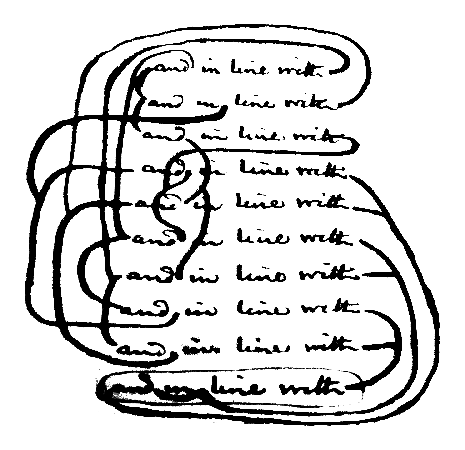
\includegraphics[width=120pt]{doc-sources/493_complex.eps}\\\vphantom{a}}
\marginnote{\lm\hspace*{2pt}%
{\scriptsize
\centering
{\setstretch{0.5}%\debugmodetrue
\ontopl{
\hk{} \hk{} \ \hk{} \ \hk{} \ \hk{} \ \hk{} \ \hk{} \ \hk{}\hphantom{and} \ \hk{}\hphantom{in} \ \hk{}\hphantom{line} \ \hk{}\hphantom{witi} \ \hk{} \ \hk{}
\setcounter{rheme}{20}\\
\hk{} \ \hk{} \ \hk{} \ \hk{} \ \hk{} \ \hk{} \ \hk{} \ \hk{}\hphantom{and} \ \hk{}\hphantom{in} \ \hk{}\hphantom{linexxxi} \ \hk{}\hphantom{with} \ \hk{} \ \hk{}
\setcounter{rheme}{40}\\
\hk{} \ \hk{} \ \hk{} \ \hk{} \ \hk{} \ \hk{} \ \ \ \,\hk{} \ \ \ \hk{}\hphantom{and} \ \hk{}\hphantom{in} \ \hk{}\hphantom{line} \ \hk{}\hphantom{with} \ \hk{} \ \hk{}
\setcounter{rheme}{60}\\
\hk{} \ \hk{} \ \hk{} \ \hk{} \ \hk{} \ \hk{} \ \hk{} \ \hk{and} \ \hk{in} \ \hk{line} \ \hk{with} \ \hk{} \ \hk{}
\setcounter{rheme}{80}\\ \\
\hk{} \ \hk{} \ \hk{} \ \hk{} \ \hk{} \ \hk{} \ \hk{} \ \hk{and} \ \hk{in} \ \hk{line} \ \hk{with} \ \hk{} \ \hk{}
\setcounter{rheme}{100}\\
\hk{} \ \hk{} \ \hk{} \ \hk{} \ \hk{} \ \hk{} \ \hk{} \ \hk{}\hphantom{xiand} \ \hk{}\hphantom{in} \ \hk{}\hphantom{line} \ \hk{}\hphantom{with} \ \hk{} \ \hk{}
\setcounter{rheme}{120}\\
\hk{} \ \hk{} \ \hk{} \ \hk{} \ \hk{} \ \hk{} \ \hk{} \ \hk{and} \ \hk{in} \ \hk{line} \ \hk{with} \ \hk{} \ \hk{}
\setcounter{rheme}{140}\\
\hk{} \ \hk{} \ \hk{} \ \hk{} \ \hk{} \ \hk{} \ \hk{} \ \hk{}\hphantom{andxxi} \ \hk{}\hphantom{in} \ \hk{}\hphantom{linex} \ \hk{}\,\hphantom{with} \ \hk{} \ \hk{}
\setcounter{rheme}{160}\\
\hk{} \ \hk{} \ \hk{} \ \hk{} \ \hk{} \ \hk{} \ \hk{} \ \hk{and} \ \hk{in} \ \hk{line} \ \hk{with} \ \hk{} \ \hk{}
\setcounter{rheme}{180}\\
\hk{} \ \hk{} \ \hk{} \ \hk{} \ \hk{} \ \hk{} \ \hk{} \ \ \ \hk{}\hphantom{and} \ \hk{}\hphantom{in} \ \hk{}\hphantom{line} \ \hk{}\hphantom{with} \ \hk{} \ \hk{}
\setcounter{rheme}{200}\\
\hk{} \ \hk{} \ \hk{} \ \hk{} \ \hk{} \ \hk{} \ \hk{} \ \hk{and} \ \hk{in} \ \hk{line} \ \hk{with} \ \hk{} \ \hk{}
\setcounter{rheme}{220}\\
\hk{} \ \hk{} \ \hk{} \ \hk{} \ \hk{} \ \hk{} \ \hk{} \ \hk{}\hphantom{and} \ \hk{}\hphantom{in} \ \hk{}\hphantom{line} \ \hk{}\hphantom{with} \ \ \ \hk{} \ \ \hk{}
\setcounter{rheme}{240}\\
\hk{} \ \hk{} \ \hk{} \ \hk{} \ \hk{} \ \hk{} \ \hk{} \ \hk{and} \ \hk{in} \ \hk{line} \ \hk{with} \ \hk{} \ \hk{}
\setcounter{rheme}{260}\\
\hk{} \ \hk{} \ \hk{} \ \hk{} \ \hk{} \ \hk{} \ \hk{} \ \hk{}\hphantom{andxx} \ \hk{}\hphantom{in} \ \hk{}\hphantom{line} \ \hk{}\hphantom{with} \ \hk{} \ \hk{}
\setcounter{rheme}{280}\\
\hk{} \ \hk{} \ \hk{} \ \hk{} \ \hk{} \ \hk{} \ \hk{} \ \hk{and} \ \hk{in} \ \hk{line} \ \hk{with} \ \hk{} \ \hk{}
\setcounter{rheme}{300}\\
\hk{} \ \hk{} \ \hk{} \ \hk{} \ \hk{} \ \hk{} \ \hk{} \ \hk{}\hphantom{and} \ \hk{}\hphantom{in} \ \hk{}\hphantom{line} \ \hk{}\hphantom{with} \ \ \ \hk{} \ \hk{}
\setcounter{rheme}{320}\\
\hk{} \ \hk{} \ \hk{} \ \hk{} \ \hk{} \ \hk{} \ \hk{} \ \hk{and} \ \hk{in} \ \hk{line} \ \hk{with} \ \hk{} \ \hk{}
\setcounter{rheme}{340}\\
\hk{} \ \hk{} \ \hk{} \ \hk{} \ \hk{} \ \hk{} \ \ \ \ \ \ \hk{} \ \hk{}\hphantom{and} \ \hk{}\hphantom{in} \ \hk{}\hphantom{line} \ \hk{}\hphantom{with} \ \hk{} \ \hk{}
\setcounter{rheme}{360}\\
\hk{} \ \hk{} \ \hk{} \ \hk{} \ \hk{} \ \hk{} \ \hk{} \ \hk{and} \ \hk{in} \ \hk{line} \ \hk{with} \ \hk{} \ \hk{}
\setcounter{rheme}{380}\\
\hk{} \ \hk{} \ \hk{} \ \hk{} \ \hk{} \ \ \ \ \ \ \hk{} \ \hk{} \ \hk{}\hphantom{and} \ \hk{}\hphantom{in} \ \hk{}\hphantom{line} \ \hk{}\hphantom{with} \hk{} \hk{} \ \hk{} \ \hk{}
\setcounter{rheme}{400}\\
\hk{} \ \hk{} \ \hk{} \ \hk{} \ \hk{} \ \hk{} \ \hk{}\,\cut{ \hk{and} \ \hk{in} \ \hk{line} \ \hk{with} } \ \hk{} \ \hk{}
\setcounter{rheme}{420}\\
\strut\hk{} \ \hk{} \ \hk{} \ \hk{} \ \hk{} \ \hk{} \ \hk{} \ \hk{}\hphantom{and} \ \hk{}\hphantom{in} \ \hk{}\hphantom{line} \ \hk{}\hphantom{with} \ \hk{} \ \hk{}
\setcounter{rheme}{440}\\
\hk{} \ \hk{} \ \hk{} \ \hk{} \ \hk{} \ \hk{} \ \hk{} \ \hk{}\hphantom{and} \ \hk{}\hphantom{in} \ \hk{}\hphantom{line} \ \hk{}\hphantom{with} \ \hk{} \ \hk{}
\setcounter{rheme}{460}
}
\downright{161}{182}\upright{161}{103}\li{103}{109}\reflexiver{109}{89}
\upright{182}{163}\li{163}{168}\downright{182}{345}\li{345}{348}\reflexiver{348}{328}
\upright{223}{8}\li{8}{12}\reflexiver{12}{91}%\li{93}{91}
\upright{223}{208}\downright{223}{386}\li{386}{388}\reflexiver{388}{368}
\upright{285}{248}\downright{285}{328}\downright{125}{248}\upright{125}{47}\li{47}{48}\reflexiver{48}{68}
\downright{144}{288}\upright{144}{28}\li{28}{31}\reflexiver{31}{71}\reflexivel{288}{368}
\reflexivel{68}{88}\reflexivel{88}{128}\rightdown{128}{189}\rightup{208}{189}\rightup{288}{269}\rightdown{189}{269}
\reflexiver{131}{151}\li{149}{151}\upright{188}{149}\nccurve[linewidth=\ligaturewidth,linecolor=\licolour,angleA=20,angleB=200]{248}{188}\reflexiver{188}{168}
\rightdown{171}{233}\rightdown{211}{233}\li{233}{394}\rightup{452}{394}\reflexivel{408}{448}\li{448}{452}
\rightdown{251}{313}\rightdown{291}{313}\li{313}{393}\rightup{432}{393}\li{430}{432}\downright{409}{430}\downright{408}{429}\rightup{429}{409}
\rightdown{331}{373}\rightup{411}{373}\li{371}{373}
\setcounter{rheme}{0}
}}
}

Defining and placing each hook in such a complex graph separately would be a stupendous task. Instead, a far more effortless strategy is to take advantage of the repetitive structures and effectively create a matrix of hooks.

A cursory glance of the graph suggests---taking into account all the bifurcations---that no single line needs more than about fourteen hooks. Since some ligatures run or bifurcate under the text lines, it is sensible to double the number of lines. Every other line needs seven empty hooks, then the words `{\lm and in line with}' in separate hooks, and five empty hooks still. In every other line, the words should be defined as \verb|\hphantom|s,\index{hphantom@\texttt{\textbackslash hphantom}} totaling a matrix of hooks 14$\times$26.

The number of hooks per line, 14, makes it difficult to calculate their relative positions in the final matrix. It makes sense to declare e.g.\,\verb|\setcounter{rheme}{100}|\index{rheme@\texttt{rheme} (counter)} at the end of the first line, \verb|{200}|\label{rhemecounter} at the end of the second and so on. Thus the relative position of a hook and the place of any \index{bifurcation}bifurcation can be figured out easily. Drawing the ligatures for the graph this way isn't trivial, but it is a lot easier than placing each hook individually.

\newthought{\texttt{PsTricks} and thus the} \texttt{egpeirce}-package allows one to define points on the plane with vectors in a polar coordinate system.\marginnote[-10pt]{\mbox{\centering
\includegraphics[width=80pt]{doc-sources/WTF_MS493.eps} \ 
\raisebox{38pt}{\lm\scriptsize\setstretch{0.8}
\centering%\debugmodetrue
\cut{ \ \ \ontop{\\
\raisebox{-5pt}{\hk{\textit{l}} \ \ \ \ \ \hk{} \ \ \ \ \ \hk{\textit{l}}}\\ \\
\raisebox{-10pt}{\hk{}} \ \ \ \ \ \ \ \,\raisebox{-8pt}{\hk{\textit{l}}} \ \ \ \ \ \ \ \,\raisebox{-10pt}{\hk{}}\\
\hk{} \ \ \ \hk{}\\
\hk{\textit{l}} \ \ \ \ \ \ \hk{\textit{l}}\\
\hk{} \ \ \ \ \ \ \ \ \ \hk{}\\
\raisebox{3pt}{\hk{\textit{l}} \ \ \ \ \ \ \,\hk{\textit{l}} \ \,\hk{} \ \,\hk{\textit{l}} \ \ \ \ \ \ \,\hk{\textit{l}}}\\ \\
\raisebox{6pt}{\hk{} \ \ \ \ \ \ \ \ \ \ \ \ \,\hk{}}\\
\cut{\,\hk{\textit{l}}\,}\\
} \ \ }
\li{1}{2}\li{2}{3}\li{3}{6}\li{6}{17}\li{17}{19}\li{19}{20}\li{20}{18}\li{18}{13}\li{13}{4}\li{4}{1}
\li{2}{5}\li{6}{10}\li{19}{16}\li{18}{14}\li{4}{9}
\li{1}{7}\li{3}{8}\li{17}{12}\li{20}{15}\li{13}{11}\li{2}{5}
\nccurve[angleA=310,angleB=180]{7}{10} \nccurve[angleA=310,angleB=80]{7}{14}
\nccurve[angleA=230,angleB=10]{8}{9}   \nccurve[angleA=230,angleB=100]{8}{16}
\nccurve[angleA=175,angleB=285]{12}{5} \nccurve[angleA=175,angleB=50]{12}{14}
\nccurve[angleA=90,angleB=220]{15}{10} \nccurve[angleA=90,angleB=320]{15}{9}
\nccurve[angleA=5,angleB=255]{11}{5}  \nccurve[angleA=5,angleB=130]{11}{16}
\setcounter{rheme}{0}
}}} By placing hooks in such points, even graphs like the one in the margin are manageable. Because these kinds of graphs are rare, this method isn't described in detail here. Please consult e.g.\ \textit{The \LaTeX\ graphics companion} for more details.

Alternatively, the matrix method described previously would work almost equally well in these situations. 

\subsection{\hspace*{-8pt}Ugly hacks}\label{uglyhacks}

In Peirce's graph-system, there are unfortunately a few cases that still escape an elegant solution. Drawing lines on paper affords a lot of freedom. Describing the graphs in code makes them look more uniform and makes their manipulation much easier. However, this method is somewhat more limited than hand-drawing and must at times compromise. Below are two examples of such compromises.\index{vscroll@\texttt{\textbackslash vscroll}}%

\newthought{The example} in\marginnote{\centering\lm\scriptsize
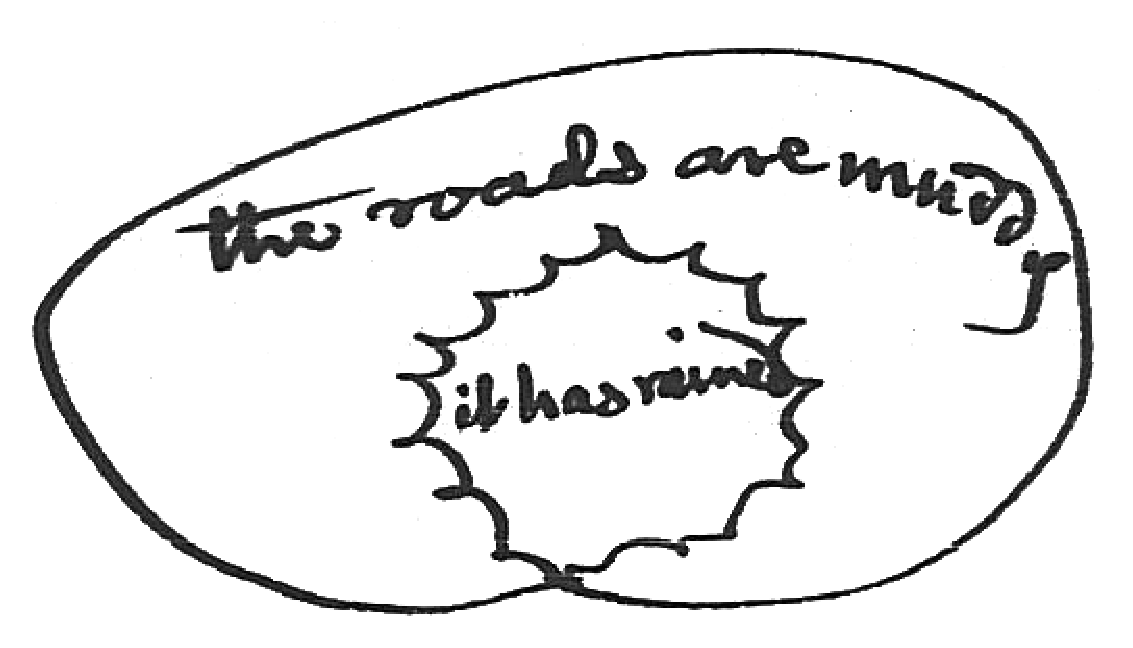
\includegraphics[scale=0.15]{doc-sources/MS481_first.eps}} the margin is a \greek{g}-graph, a scroll, that is wavy in the inner cut. Perhaps surprisingly, this is very difficult to solve.

\makeatletter
\def\tx@ziggy{ \tx@setStrokeTransparency ziggy }% The bridge-ligature with a line. This code is a bit overkill, but works.
\@namedef{psas@z}{%
  /ziggy {%
    CLW mul add dup 2 div
    /x ED mul neg
    /y ED
    /mtrx CM def
    0 CLW
    2 div T x y mul 0 ne { x y scale } if
    0.15 -2.5 moveto
    -0.15 -1 lineto
    0.15 0.5 lineto
    0.4 setlinewidth
    mtrx setmatrix stroke 0 2.8 moveto } def
  \psk@rbracketlength\space \psk@tbarsize\space \tx@ziggy
}
\makeatother

\texttt{PostScript} does have a mechanism for drawing zigzag \textit{lines}, but the difficulty here is that the cut is also \textit{curved}. The zigzag lines can be bent on the arc of a a circle, but the code does this in an idiosyncratic way that's hard to generalize to an arbitrary curve. There is no algebraic solution to calculate a \textit{general} wavy curve that I would be aware of. \texttt{PostScript} \textit{is} an extremely powerful programming language and it can even solve (certain types of) differential equations automatically. I do have a nagging feeling that I must have embarrassingly overlooked something really obvious.

Of course---for our purposes---the zigzagging perimeter wouldn't have to form an actual \textit{continuous} line. Merely a visually convincing semblance would suffice. And this is exactly what's done here. For now, the package must resort to a crude approximation.\bigskip

\noindent I use one of the methods that \textit{do} allow us to put zigzagging elements on an arbitrary curve. There is, however, a general problem in this approach with the discrete elements that form the ersatz zigzag-line. They consists of a `zig'~(\,\psscalebox{0.5}{\begin{pspicture}(0,-0.1)(0.15,-0.1)\psline[linewidth=0.8pt](0,0.02)(0.15,0.2)\end{pspicture}}\,), a `zag' ~(\,\psscalebox{0.5}{\begin{pspicture}(0,-0.1)(0.15,-0.1)\psline[linewidth=0.8pt](0,0.2)(0.15,0.02)\end{pspicture}}\,) or a `zigzag'~(\,\psscalebox{0.5}{\begin{pspicture}(0,-0.1)(0.3,-0.1)\psline[linewidth=0.8pt](0,0.02)(0.15,0.2)(0.3,0.02)\end{pspicture}}\,) repeated one after another. Thus the line is---for lack of a better word---\textit{quantized} on the zigs or zags\marginnote[60pt]{ \ \ \ \ \ \ \ \ \ \ \Rnode{Q}{} \ \ \ \psbezier[linestyle=none,ArrowInside=-z,ArrowInsideNo=38](0,-1)(-2,0)(-2,2)(2,2)(2,0)%(2,0)(0,3)(3,0)(1,0)
} (\&~this is one of the reasons why it's so difficult to come up with a simple algebraic solution). With this method one has to always guess or estimate the number of elements needed.

One possibility would be to create a new zigzag arrow and fill a line with it:\psline[ArrowInside=-z,ArrowInsideNo=11,linestyle=none](1.55,0.1)(0,0.1) \ \ \ \ \ \ \ \ \ \ \ \ \ \ . This method applies also to B\'{e}zier curves of\Rnode{P}{}\penalty-10000 arbitrary curvature. \texttt{PostScript}\noticeline{220}{P}{Q}\ has a method of computing tangents to a curve at different specified points. The tangents could be used to compute control points for a B\'{e}zier curve approximating the path of the zigzag segment. This, however, is unnecessarily complex and would involve \textit{also} guesstimating the beginning and end points.

The mechanism employed for now uses a command that makes \textit{text} follow a curved path. After the normal scroll has been drawn, an additional line is drawn through the inner part of the cut. This line has some text in it that draws the ersatz zigzag line.\marginnote{\centering\lm\scriptsize
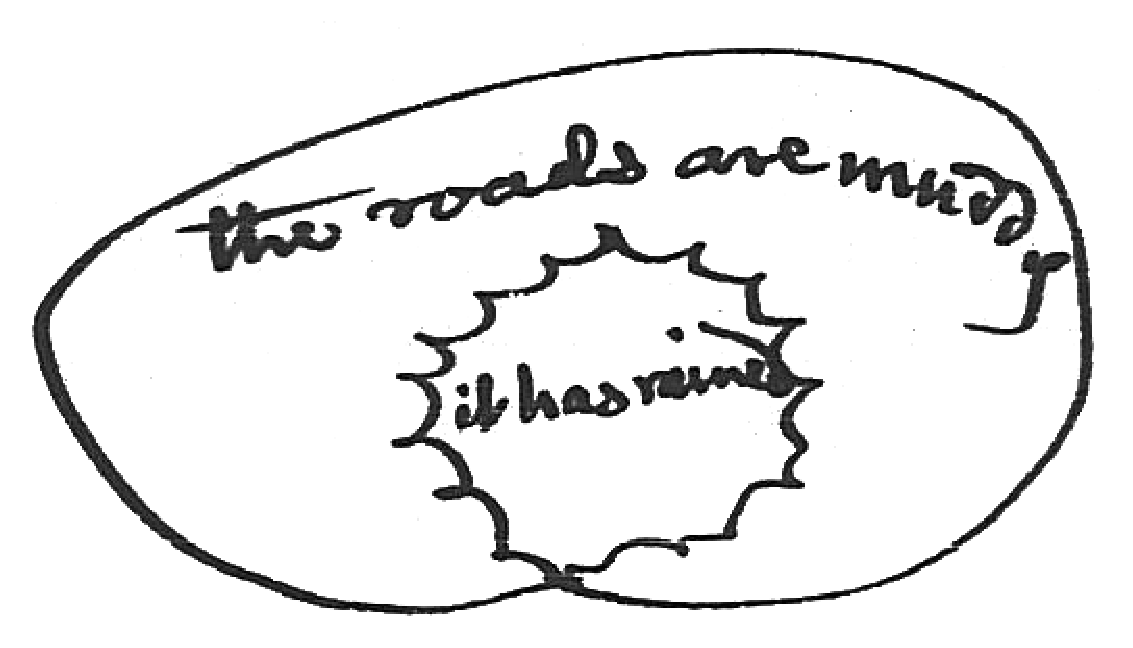
\includegraphics[scale=0.15]{doc-sources/MS481_first.eps}\\\mbox{ }\\{\setstretch{0.3}\begin{Bcenter}\DefNodes{A}{\vphantom{\Large A} \ The roads are muddy \ }\\ \DefNodes{B}{\strut\hphantom{it has rainedxx}}\\ \DefNodes{C}{ \strut It has rained \ontop{\strut\\\strut\\\strut\\\strut\\\strut} }\\ \DefNodes{D}{\strut\hphantom{ The roads are muddyxx}}\end{Bcenter}
\pspolygon[linearc=.18,linewidth=.2pt](A-tl)(A-tr)(D-br)(C-bl)(B-ml)(B-mr)(C-br)(D-bl)
\pstextpath[c](0,0){\psline[linearc=.18,linestyle=none](D-br)(C-bl)(B-ml)(B-mr)(C-br)(D-bl)}{\vv\vv\vv\vv\vv\vv\vv\vv\vv\vv\vv\vv\vv\vv\vv\vv\vv\vv\vv\vv\vv\vv\vv\vv\vv\vv\vv\vv\vv\vv\vv\vv\vv\vv\vv\vv\vv\vv\vv\vv\vv\vv\vv\vv\vv\vv\vv\vv\vv\vv\vv\vv\vv\vv\vv\vv\vv\vv\vv\vv}
}\\\strut\\\strut\\\strut\\%
{\setstretch{0.2}\begin{Bcenter}\DefNodes{E}{\vphantom{\Large A} \ \hphantom{The roads }\pstextpath[c](0,0){\pscurve[curvature=2 0 0,linestyle=none](-1.5,-0.4)(0,0.4)(1.5,-0.4)}{The roads are muddy}\hphantom{are muddy} \ }\\ \DefNodes{F}{\strut\hphantom{it has ra}}\\ \DefNodes{G}{ \ontop{It has\\ rained\\\vphantom{p}} }\\ \DefNodes{H}{\strut\hphantom{ The roads are muxxxx}}\end{Bcenter}
\psccurve[curvature=1 0 0,arcsep=10pt,linewidth=\cutwidth,linecolor=\cutcolour](E-tl)(E-tr)(H-br)(G-bl)(F-ml)(F-mr)(G-br)(H-bl)
\pstextpath[c](0,0){\pscurve[curvature=1 0 0,arcsep=10pt,linestyle=none](E-tr)(H-br)(G-bl)(F-ml)(F-mr)(G-br)(H-bl)(E-tl)}{\vv\vv\vv\vv\vv\vv\vv\vv\vv\vv\vv\vv\vv\vv\vv\vv\vv\vv\vv\vv\vv\vv\vv\vv\vv\vv\vv\vv\vv\vv\vv\vv\vv\vv\vv\vv\vv\vv\vv\vv\vv\vv\vv\vv\vv\vv\vv\vv\vv}%
}} Here, the zigzags are repetitions of the caret (\,\^\,) whose background is filled to hide the line, that are lowered and kerned so that they can be made to form a continuous-looking line:\raisebox{4pt}{\vv\hspace*{-1pt} \vv\hspace*{-1pt} \vv\hspace*{-1pt} \vv\hspace*{-1pt} \vv\hspace*{-1pt} \vv\hspace*{-1pt} \vv\hspace*{-1pt} \vv\hspace*{-1pt} \vv\hspace*{-1pt} \vv\hspace*{-1pt} \vv } \,. Since this is a complex operation, there's a command (\verb|\vv|) that does precisely that, one caret at a time.\index{vv@\texttt{\textbackslash vv}|textbf}

The command for the zigzag curve in the \texttt{longscroll} is:\index[visual]{f@
{\setstretch{0.2}\begin{Bcenter}\DefNodes{E}{\vphantom{\Large A} \ \ }\\ \DefNodes{F}{\strut \ \ \ }\\ \DefNodes{G}{\strut \ \ }\\ \DefNodes{H}{\strut \ \ \ }\end{Bcenter}}
\psccurve[curvature=1 0 0,arcsep=10pt,linewidth=\cutwidth,linecolor=\cutcolour](E-tl)(E-tr)(H-br)(G-bl)(F-ml)(F-mr)(G-br)(H-bl)
\pstextpath[c](0,0){\pscurve[curvature=1 0 0,arcsep=10pt,linestyle=none](E-tr)(H-br)(G-bl)(F-ml)(F-mr)(G-br)(H-bl)(E-tl)}{\vv\,\vv\,\vv\,\vv\,\vv\,\vv\,\vv\,\vv\,\vv\,\vv\,\vv\,\vv\,} \ \ }
\medskip

\noindent\verb|\pstextpath[c](0,0){\psline[linearc=.18,linestyle=none]|\\
\verb|(A\egatn-tr)(D\egatn-br)(C\egatn-bl)(B\egatn-ml)(B\egatn-mr)| \verb|(C\egatn-br)(D\egatn-bl)(A\egatn-tl)}{\vv\vv\vv\vv\vv\vv| \dots \verb|}|\medskip

\noindent For the normal \texttt{scroll}, replace the \verb|\psline| with a \verb|\pscurve[curvatu| \verb|re=1 0 0,arcsep=10pt,linestyle=none]|.

This places the carets onto the line defined by the usual scroll sequence. Only the inner cut should be zigzagged. Since the intersection point doesn't have a referenceable coordinate, the carets are made to emanate from the middle of the line (with the \verb|[c]| option). By drawing just enough carets, they will stop at the intersection.

This is an ugly hack: it does the trick, albeit not very elegantly.

\newthought{Peirce's manuscripts include} scrolls and cuts that have an emptied or blackened inner cut (``blot''\index{blot|textbf} as Peirce called it). This expresses the \textit{pseudograph} and is thus entirely and fundamentally different idea from shaded cuts made with \verb|\colouredcuts| (page~\pageref{colouredboolean}).\index[visual]{e@{\psset{fillstyle=oefill,fillcolor=black}\vscroll{ \ }{ \ }} \ \  {\psset{fillstyle=eofill,fillcolor=black}\vscroll{ \ }{ \ }} \ }\label{colouredscrolls}

There are two special fillrules in \texttt{PostScript}, \texttt{oefill} and \texttt{eofill} that fill evenly or oddly self-intersecting areas. Introducing these through \verb|\psset{}| allows you to fill the inner cut of any scroll.\marginnote[-80pt]{%
{\lm\ontopl{%
{\scriptsize\texttt{ \textbackslash{}vscroll\{A\}\{B\}}}\\\\
\vscroll{A}{B}\\\\\\\\
{\scriptsize\texttt{\{\textbackslash{}psset\{fillstyle=\uline{eo}fill,fillcolor=black\}}}\\
{\scriptsize\texttt{ \textbackslash{}vscroll\{A\}\{B\}\}}}\\\\
{\psset{fillstyle=eofill,fillcolor=black}\vscroll{A}{B}}\\\\\\\\
{\scriptsize\texttt{\{\textbackslash{}psset\{fillstyle=\uline{oe}fill,fillcolor=black\}}}\\
{\scriptsize\texttt{ \textbackslash{}vscroll\{A\}\{B\}\}}}\\\\
{\psset{fillstyle=oefill,fillcolor=black}\vscroll{A}{B}}
}}}

Notice that any content in the singly cut area is painted over in this method and would have to be reinserted through other means.\medskip

\noindent An alternative way to fill the inner cut of a scroll exists that does not fill the singly cut area. Here you specify a \texttt{solid} fillstyle and make it traverse \textit{only} the inner cut. This is a rather hacky way to achieve the desired effect though, since you have to figure out the intersection point manually by trial and error.

Recall that the points \verb|\DefNodes| creates are internally simply references to a pair of coordinate points. You can try to find the intersection using raw coordinates. In the first scroll below, this happens to be at \texttt{-0.26,-0.32}, so \verb|\psccurve[curvature=1 0 0,linewidth=.2| \verb|pt,fillstyle=solid,fillcolor=black](-0.26,-0.32)(C\egatn-bl)|\break \verb|(B\egatn-ml)(B\egatn-mr)(C\egatn-br)(-0.26,-0.32)| fills the cut:\index{defnodes@\texttt{\textbackslash DefNodes}}\index{egatn@\texttt{\textbackslash egatn}}\bigskip

%\begin{center}
%\noindent{\setstretch{0.3}
%\begin{Bcenter}\DefNodes{A}{ \ \sz{A}\vphantom{a} \ }\\ \DefNodes{B}{ \ \,}\\ \DefNodes{C}{ \ \ \ }\\ \DefNodes{D}{\strut\hphantom{aaa}}\end{Bcenter}
%\psccurve[curvature=1 0 0,arcsep=10pt,linewidth=.2pt](A-tl)(A-tr)(D-br)(C-bl)(B-bl)(B-br)(C-br)(D-bl)
%\psccurve[curvature=1 0 0,arcsep=10pt,linewidth=.2pt,fillstyle=solid,fillcolor=black](-0.38,-0.23)(C-bl)(B-ml)(B-mr)(C-br)(-0.38,-0.23)
%}\hfill
\noindent \ \ {\vscroll{ \sz{A} }{B}%
\psccurve[curvature=1 0 0,arcsep=10pt,linewidth=.2pt,fillstyle=solid,fillcolor=black](-0.26,-0.32)(C\egatn-bl)(B\egatn-ml)(B\egatn-mr)(C\egatn-br)(-0.26,-0.32)}
\hfill
{\setstretch{0.3}
\begin{Bcenter}\DefNodes{A}{ \ \sz{A}\vphantom{a} \ }\\ \DefNodes{B}{\,}\\ \DefNodes{C}{}\\ \DefNodes{D}{\strut\hphantom{aaa}}\end{Bcenter}
\psccurve[curvature=1 0 0,arcsep=10pt,linewidth=.2pt](A-tl)(A-tr)(D-br)(C-bl)(B-bl)(B-br)(C-br)(D-bl)
\psccurve[curvature=1 0 0,arcsep=10pt,linewidth=.2pt,fillstyle=solid,fillcolor=black](-0.402,-0.053)(C-bl)(B-ml)(B-mr)(C-br)(-0.402,-0.053)
}\hfill
{\setstretch{0.3}
\begin{Bcenter}\DefNodes{A}{ \ \sz{A}\vphantom{a} \ }\\ \DefNodes{B}{}\\ \DefNodes{C}{}\\ \DefNodes{D}{\strut\hphantom{aaa}}\end{Bcenter}
\psccurve[curvature=1 0 0,arcsep=10pt,linewidth=.2pt](A-tl)(A-tr)(D-br)(B-bl)(B-br)(D-bl)
}\hfill
{\setstretch{0.1}
\begin{Bcenter}\DefNodes{A}{ \ \sz{A}\vphantom{a} \ }\\ \DefNodes{B}{\,}\\ \DefNodes{C}{\vphantom{a}}\\ \DefNodes{D}{\strut\hphantom{aaa}}\end{Bcenter}
\psccurve[curvature=1 0 0,arcsep=10pt,linewidth=.2pt](A-tl)(A-tr)(D-br)(C-bl)(D-bl)
}\hfill
\raisebox{2pt}{\cut{ \,\strut\sz{A} \,}}\hfill 
\raisebox{2pt}{\cut{ \ }}\hfill \raisebox{3.5pt}{.}
%\end{center}

\newpage
\notinlinetrue

\section{\hspace*{-15pt}Some difficult cases and their solutions}

Next I will discuss a few recurring \textit{general types} of problematic cases that arise when transcribing graphs from manuscripts. Some of these problems can be solved by changing mutable parameters of the package. Others require slightly more involved methods.

More specific cases of difficult graphs and their solutions are dealt with in the examples.

\subsection{\hspace*{-8pt}Mutable parameters of the package}

The \texttt{egpeirce}-package includes many predefined parameters and dimensions that can be reset if needed. Change parameters with \verb|\renewcommand{\<|{\Fontauri parametername}\verb|>}{<|{\Fontauri value}\verb|>}|. Dimensions are reset by \verb|\setlength{\<|{\Fontauri dimensionname}\verb|>}{<|{\Fontauri value}\verb|>}|. You must specify all dimensions with a \textit{unit}. Parameters can be integers, fractions or strings.

These changes have a global scope and must be explicitly reset even to get the default values back. You can of course change them for only a small period, even inside or in the middle of a graph.

Below, the initial default value of the parameter or dimension is written in the margin for easy and fast reference.

\newthought{In most of} Peirce's manuscripts, the cuts are drawn with a very fine black line (with a pointed nib or the narrow side) and the ligatures with a distinctly heavier pen or wider nib. This is emulated by the package. Dimensions called \texttt{cutwidth} and \texttt{ligaturewidth} are in charge of the width of the cut and ligature.\marginnote[-20pt]{\texttt{%
\textbackslash{}setlength\{\textbackslash{}cutwidth\}\{0.2pt\}\\%
\textbackslash{}setlength\{\textbackslash{}ligaturewidth\}\{1.2pt\}%
}}\index{cutwidth@\texttt{\textbackslash cutwidth} (dim)|textbf}%
\index{ligaturewidth@\texttt{\textbackslash ligaturewidth} (dim)|textbf}%


The colour of a coloured cut\label{colouredcutcolour} is defined with a parameter called \texttt{cutxfillcolour}.\marginnote{\texttt{\textbackslash{}renewcommand\{\textbackslash{}cutxfillcolour\}\{gray\}}} As was mentioned earlier, when cuts are delimited with a coloured region by declaring \verb|\colouredcutstrue|, there is no line drawn to distinguish them. Sometimes, especially in \greek{g}-graphs there are however heavy lines around a coloured region to specify a cut. To ease the use of this, you can increase the value of the \texttt{cutxwidth}-dimension and set the \texttt{cutxcolour} parameter to a suitable colour\marginnote[-30pt]{\texttt{%
\textbackslash{}setlength\{\textbackslash{}cutxwidth\}\{0.01pt\}\\\\%
\textbackslash{}renewcommand\{\textbackslash{}cutxcolour\}\{white\}%
}}.\index{cutxfillcolour@\texttt{\textbackslash cutxfillcolour} (param)|textbf}%


It is also possible to fill a cut with a pattern instead of a solid colour.\index{xfillstyle@\texttt{\textbackslash xfillstyle} (param)|textbf} This is defined with the\marginnote{\texttt{\textbackslash{}renewcommand\{\textbackslash{}xfillstyle\}\{solid\}}} \texttt{xfillstyle} parameter. See the next section for more details.

Sometimes Peirce drew the cuts with a dark blue ink. Ligatures are also drawn in colours other than black, at least bright red and brown ones exist too. The colour of a cut is defined with a parameter called \texttt{cutcolour}\marginnote[-10pt]{\texttt{%
\textbackslash{}renewcommand\{\textbackslash{}cutcolour\}\{black\}\\%
\textbackslash{}renewcommand\{\textbackslash{licolour\}\{black\}}%
}} and the colour of ligatures with \texttt{licolour}.\index{cutcolour@\texttt{\textbackslash cutcolour} (param)|textbf}%
\index{licolour@\texttt{\textbackslash licolour} (param)|textbf}%

Finally, all vertical scrolls have reduced lineheight. Since all vertical scrolls have five layers, a logical choice would be \texttt{0.2}\marginnote{\texttt{\textbackslash{}renewcommand\{\textbackslash{}scrollstretch\}\{0.3\}}}.\index{scrollstretch@\texttt{\textbackslash scrollstretch} (rational)|textbf} For \ae sthetic reasons the default is slightly higher. Very much smaller values will look bad and can create problems with the arcs. 

\subsection{\hspace*{-8pt}Some handy PostScript commands}

Some\label{handyps} \greek{g}-graphs have cuts whose lines are not solid or whose areas are coloured. Since these cases are rare and not very consistent in appearance, there isn't a single parameter that governs this behaviour.

Whenever you want to draw a nonsolid cut, you must first declare \verb|\psset{linestyle=dashed,dash=<|{\Fontauri x}\verb|>pt}| before the cut. The value of~\verb|<|{\Fontauri x}\verb|>| determines the length of the dashes. Changing the \verb|linestyle| parameter to \verb|dotted| draws dots instead of dashes.\marginnote[-30pt]{%
\cut{\cut{\cut{ \ \ \ }}} \ \ \ %
\cut{\psset{linestyle=dashed,dash=4pt}\cut{\psset{linestyle=solid}\cut{ \ \ \ }}} \ \ \ %
\cut{\setlength{\cutwidth}{.5pt}\psset{linestyle=dotted,dotsep=1pt}\cut{\setlength{\cutwidth}{.2pt}\psset{linestyle=solid}\cut{ \ \ \ }}} \ \ \ %
\psset{linestyle=dashed,dash=1pt}\cut{\setlength{\cutwidth}{.5pt}\psset{linestyle=dotted,dotsep=1pt}\cut{\setlength{\cutwidth}{.2pt}\psset{linestyle=dashed,dash=2pt}\cut{ \ \ \ }}}\psset{linestyle=solid}%
}

Declare \verb|\psset{linestyle=solid}| to get solid lines back in the middle of a graph. Values of \verb|cutwidth| and \verb|cutcolour| hold for the dashed or dotted cuts also.

To draw coloured cuts you just need to change the \texttt{cutxfillcolour}\label{gammacolouring} parameter to a different colour and remember to draw all the cuts with the \verb|\cutx{}| command\marginnote[20pt]{%
\colouredcutstrue%
\setlength{\cutxwidth}{0.2pt}%
\renewcommand{\cutxcolour}{black}%
\renewcommand{\cutxfillcolour}{lightblue}\cutx{%
\renewcommand{\cutxfillcolour}{lightred}\cutx{%
\renewcommand{\cutxfillcolour}{lightblue}\cutx{ \ \ \ }}}%
\renewcommand{\cutxfillcolour}{white}\renewcommand{\xfillstyle}{crosshatch*}%
\psset{hatchwidth=0.1pt,hatchsep=2pt,hatchangle=45} \ \ \ \ %
\cutx{\psset{hatchwidth=0.1pt,hatchsep=2pt,hatchangle=90}%
\renewcommand{\xfillstyle}{vlines*}\cutx{\psset{hatchwidth=0.1pt,hatchsep=2pt,hatchangle=45}%
\renewcommand{\xfillstyle}{crosshatch*}\cutx{ \ \ \ }}} \ \ \ %
\renewcommand{\cutxfillcolour}{white}\renewcommand{\xfillstyle}{vlines*}%
\psset{hatchwidth=0.1pt,hatchsep=2pt,hatchangle=45}
\cutx{\psset{hatchwidth=0.1pt,hatchsep=2pt,hatchangle=135}%
\cutx{\psset{hatchwidth=0.1pt,hatchsep=2pt,hatchangle=45}%
\cutx{ \ \ \ }}} \ \ \ %
\setlength{\cutxwidth}{0.01pt}
\renewcommand{\cutxcolour}{white}
\renewcommand{\cutxfillcolour}{gray}
\colouredcutsfalse%
}. %
To fill a cut with a pattern, change the \texttt{xfillstyle}-parameter to a suitable option and give a value to options of \texttt{hatchwidth}, \texttt{hatchsep} and \texttt{hatchangle} with \verb|\psset{}|. See the \texttt{PSTricks}-documentation for more options and examples.


Notice that unlike the parameters discussed in the previous section, \verb|\psset{}| \textit{is} sensitive to scoping, so you can also limit all the effects by enclosing it in curly brackets.



\newthought{As was mentioned earlier}, \ PostScript does handle drawing arbitrarily curved lines but requires that the end angles be always defined\label{ncarc}. The \verb|\nccurve[]{}{}| command does this.\index{nccurve@\texttt{\textbackslash nccurve}|textbf}

\verb|nccurve| accepts line properties as \textit{optional arguments}, so give them comma separated inside the square brackets. Specify linewidth and colour as \texttt{linewidth=\textbackslash{}ligaturewidth,linecolor=\textbackslash{}licolour} so that changes in these parameters also effect these ligatures. The entry and exit angles are defined as \verb|angleA=<|{\Fontauri degrees}\verb|>| and \verb|angleB=<|{\Fontauri degrees}\verb|>|. Angle directions follow those of the normal mathematical unit circle\Rnode{A}{}\marginnote[-15pt]{\centering\sz{%
\psline[linewidth=0.5pt](0,0)(0.6;22.5)%
\psline[linewidth=0.5pt](0,0)(0.6;68.5)%
\psline[linewidth=0.5pt](0,0)(0.6;112.5)%
\psline[linewidth=0.5pt](0,0)(0.6;157.5)%
\psline[linewidth=0.5pt](0,0)(0.6;202.5)%
\psline[linewidth=0.5pt](0,0)(0.6;247.5)%
\psline[linewidth=0.5pt](0,0)(0.6;292.5)%
\psline[linewidth=0.5pt](0,0)(0.6;337.5)%
\pscircle*[linecolor=white,fillcolor=white,linewidth=0pt](0,0){0.5}
\psline[linewidth=0.5pt](0,0)(0.7;45)\rput(0.9;45){\tiny45\textdegree}%
\psline[linewidth=0.5pt](0,0)(0.7;135)\rput(0.9;135){\tiny135\textdegree}%
\psline[linewidth=0.5pt](0,0)(0.7;225)\rput(0.9;225){\raisebox{-6pt}{\Rnode{B}{}}\raisebox{8.5pt}{}\tiny225\textdegree}%
\psline[linewidth=0.5pt](0,0)(0.7;315)\rput(0.9;315){\tiny315\textdegree}%
\pscircle*[linecolor=white,fillcolor=white,linewidth=0pt](0,0){0.4}
\psline[linewidth=0.6pt](0.3,0)(0.8;0)\rput(1.3;0){0\textdegree/360\textdegree}%
\psline[linewidth=0.6pt](0,0.3)(0.8;90)\rput(1;90){90\textdegree}%
\psline[linewidth=0.6pt](-0.3,0)(0.8;180)\rput(1.1;180){180\textdegree}%
\psline[linewidth=0.6pt](0,-0.3)(0.8;270)\rput(1;270){270\textdegree}%
\pscircle[linewidth=0.4pt](0,0){0.555}
}}. That is, to the `right' it is 0\textdegree\ or 360\textdegree, for `up' it's 90\textdegree\ and so on\noticeline{225}{A}{B}. The destination hook numbers are given in the usual way.

One situation where you may have to use \verb|nccurve| is if the lines of bridges\index{bridge} do not meet at right angles.\index{debugmode@\texttt{\textbackslash debugmode} (boolean)}%
\marginnote[10pt]{\centering%
\debugmodetrue%
\ontop{\hk{\rc}\\\\\hk{\rc}} \ \ \ \ \ \hk{\rc} \ \ \ \ \ \ontop{\hk{\rc}\\\\\hk{\rc}}%
\setcounter{rheme}{0}\debugmodefalse\\$\downarrow$\\\renewcommand{\licolour}{lightgray}
\ontop{\hk{\rc}\\\\\hk{\rc}} \ \ \ \ \ \hk{} \ \ \ \ \ \ontop{\hk{\rc}\\\\\hk{\rc}}%
\rightdown{1}{3}\downright{3}{5}\sligature[-b]{2}{3}\sligature[b-]{3}{4}
\reflexivel{1}{2}\reflexiver{4}{5}
\setcounter{rheme}{0}\\$\downarrow$\\\renewcommand{\licolour}{black}
\ontop{\hk{}\\\\\hk{}} \ \ \ \ \ \hk{} \ \ \ \ \ \ontop{\hk{}\\\\\hk{}}%
\nccurve[linewidth=\ligaturewidth,linecolor=\licolour,angleA=0,angleB=135]{1}{3}%
\nccurve[linewidth=\ligaturewidth,linecolor=\licolour,angleA=315,angleB=180]{3}{5}%
\nccurve[linewidth=\ligaturewidth,linecolor=\licolour,angleA=0,angleB=225]{-b}{2}{3}%
\nccurve[linewidth=\ligaturewidth,linecolor=\licolour,angleA=45,angleB=180]{b-}{3}{4}%
\reflexivel{1}{2}\reflexiver{4}{5}
\setcounter{rheme}{0}
}
The example ligature in the margin exemplifies this. The graph has five hooks. Using the shorthands makes the crossing looks strange, since they force it to be perpendicular. \verb|nccurve| enables the crossing to be effectively rotated by 45\textdegree. The bridged parts of the example are drawn with the commands:
\smallskip

\noindent\hspace*{5pt}\verb|\nccurve[linewidth=\ligaturewidth,linecolor=\licolour,|\break \hspace*{52pt}\verb|angleA=0,angleB=225]{-b}{2}{3}|

\noindent\hspace*{5pt}\verb|\nccurve[linewidth=\ligaturewidth,linecolor=\licolour,|\break \hspace*{52pt}\verb|angleA=45,angleB=180]{b-}{3}{4}|
\smallskip

\noindent The entry and exit angles (\verb|225| and \verb|45|) define a smooth curve through the center hook. Notice that when you use \verb|nccurve|, the bridge (or the gap) declaration must be in curly brackets instead of square ones.

\newpage
\fancyhead[RE]{\scshape\newlinetospace{\MakeTextLowercase{Peirce's logical symbols}}\quad\thepage}%WORKS
\section{\hspace*{-15pt}Peirce's logical symbols}

The package includes commands that print symbols Peirce developed for his logical system. Peirce was fastidious about the details and appearance of these symbols and signs, and every effort has been made to make the glyphs appear as close as possible to Peirce's descriptions and examples. When needed, alternative variants of symbols are also provided.\label{symbolspage}

These symbols are not included in the package as new fonts but rather as vectorized pictures. This substantially decreases work need\-ed to define them and also means that you don't need to separately install a new typeface to use them. All the symbols are contained within the package.\medskip

\noindent This technique does have two setbacks, however.

First, a separate mechanism for scaling the symbols had to be created. The symbols respond to the sizing commands (\verb|\tiny|\ \dots\,\verb|\Huge|) and they also scale whenever your \texttt{.cls} file tells \LaTeX\ to change font sizes (e.g.\ inside footnotes and headers). If the symbols appear to be \textit{overall} too small or too large compared to the typeface you use, you can change their size relative to it by redefining a command called \texttt{commoncoefficient}.\marginnote{{\texttt{\textbackslash{}renewcommand\{\penalty-10000 \textbackslash{}commoncoefficient\}\{\texttt{<{\Fontauri r}>}\}}}\hfill{\Fontauri r}\,$ \in \mathbbb{R}^+_{>0}$\\\\ As the name suggests, it is a scaling coefficient common for all the sizes. The default is, obviously, \texttt{1}.} Internally, the scaling mechanism tracks the \verb|\f@size| macro, which should be a reliable source for size information. If it nevertheless causes problems, you can turn the scaling off by setting the Boolean flag \verb|\scaledsymbols| to \texttt{false}. This won't effect the \verb|commoncoefficient| command, so you can use it to scale the symbols independently.\index{scaledsymbols@\texttt{\textbackslash scaledsymbols} (boolean)|textbf}\index{commoncoefficient@\texttt{\textbackslash commoncoefficient} (rational)|textbf}

Secondly, you \textit{might} get error messages when you use the symbol commands e.g.\ in places where \LaTeX\ needs to use external files, such as in the sectioning commands (which write to the~\texttt{.toc} file) and indexing commands (that use the~\texttt{.idx} files).\marginnote{\gray\texttt{\textbackslash{}part\{Part text \textbackslash{}protect\textbackslash<{\Fontauri symbolname}>\}\\\\\textbackslash{}section\{Section text \textbackslash{}protect\textbackslash<{\Fontauri symbolname}>\}\\\\\textbackslash{}index\{\textbackslash{}protect\textbackslash<{\Fontauri symbolname}>\}}} If this happens, you can easily solve these errors simply by preceding the symbol commands with the standard \LaTeX\ command \verb|\protect|.\index{protect@\texttt{\textbackslash protect}} This is fundamentally due to the symbol commands being `fragile' and \LaTeX\ forcing their expansion too early. The concepts of command expansion, execution, and `fragility' are too complex and low-level to be dealt with here. Be aware that early expansion---whenever it happens---will invariably result in copious amounts of errors grave enough to stop compilation. Use e.g.\ the \verb|\protect| or \verb|\expandafter| commands when needed.\marginnote[16pt]{\lm%
$\breve{\weirdthree} \hfill \bar{\reversedragonhead}$ \hfill A $\hat{\boxxoperator{l}}$ B \hfill $\overline{\varinclusion}$ \hfill $\widehat{a \aggregate b}$ \hfill $a\ \underleftarrow{\Ppropto}\ b$ \hfill $\displaystyle\prod_{\aggregate\in\ i}^{\flatinfty}$
\\\\
$\overbrace{a\ \aggregate\ b\ \aggregate\ c\ \cdots\ k\ \aggregate\ l\ \aggregate\ m }$
}\medskip

\noindent Symbols that need to---at least in principle---interact with standard mathematical compositioning and typesetting commands available in \LaTeX\ (\verb|\hat{}|, \verb|\bar{}|, \verb|\overline{}|, etc.), do play nice with them.

\newthought{Next, lists of} the symbol commands and symbols are presented. The lists do not give the definitions, semantics or explanations for the symbols. References to manuscripts are provided to that end. As was mentioned in the beginning, this documentation tacitly assumes that the reader is familiar with existential graphs and Peirce's logic.

Some of these references are unique, but most symbols (and even their definitions) exist in multiple manuscripts. Further notes about some symbols are presented in footnotes.

\newthought{First, a list} of simple symbol commands for the linear notation:\vspace*{0.5cm}\marginnote[30pt]{%
\textsuperscript{9} This variant exists \textit{only} for use in the \texttt{\textbackslash{}agoverline\{\}} commands below, and does \textit{not} appear in Peirce's manuscripts as such.\\\\
\textsuperscript{10} The capital `\texttt{P}' in the command names denotes Peirce's variant of an already existing \LaTeX\ command.

This is Peirce's preferred version for the constellation symbol of Aries.\\\\
\textsuperscript{11} This is merely a typographical variant of the \textbackslash\texttt{implicates} command. Peirce's description for it (from a letter to Paul Carus in Oct.~1898) was: ``The character\,[\,\dots]\,ought to have a somewhat Chinese effect. I have drawn the longer line pointed at both ends. But I don't know but it would look better blunt at the left. If so cut that edge must not be vertical but slanting'', and a hand-drawn sketch of this variant is also provided.

In almost all manuscripts though, the symbol resembles more the `non-cursive' variant.\\\\
\textsuperscript{12} These symbols are Peirce's own modifications on his father's notation, for the mathematical constants~$e$ and~$\pi$ respectively (found e.g. in the \textit{Century Dictionary} under the entry `\textit{Notation}').

The identity $\napierianbase^{{\scriptsize\Pratiocircdia}}$ = (--1)\textsuperscript{--${\sqrt{ \ \ \ \ }}$}\kern-6.1pt\textsuperscript{--1} holds.% This sucks, but the garamond oldstyle letters look better here than math mode.
}

\renewcommand{\arraystretch}{1.2}
\setlength\arrayrulewidth{0.1pt}
\begin{tabular}{lcr}%\rowcolor{lightgray}%
Command name & Symbol & From manuscript\\
\hline
\verb|\aggregate| & \aggregate & \textsc{ms\,293}\\
\verb|\varaggregate|\ \textsuperscript{9} & \varaggregate &\\
\verb|\Paries|\ \textsuperscript{10} & \Paries & \textsc{ms\,530}\\
\verb|\dragonhead| & \dragonhead & \textsc{ms\,501}\\
\verb|\reversedragonhead| & \reversedragonhead  & \textsc{ms\,501}\\
\verb|\flatinfty| & \flatinfty & \textsc{ms\,530}\\
\verb|\fsymbol| & \fsymbol & \textsc{ms\,l\,224}\\
\verb|\implicates| & \implicates & \textsc{ms\,430}\\
\verb|\cursiveimplicates|\ \textsuperscript{11}  & \cursiveimplicates & \textsc{ms\,l\,387}\\
\verb|\varinclusion| & \varinclusion & \textsc{ms\,530}\\
\verb|\Ppropto| & \Ppropto & \textsc{ms\,530}\\
\verb|\Pinversepropto| & \Pinversepropto & \textsc{ms\,530}\\
%\verb|\varsubsumption| & \varsubsumption & \textsc{ms\,nnn}\\
\verb|\varwedge| & \varwedge & \textsc{ms\,530}\\
\verb|\weirdone| & \weirdone & \textsc{ms\,530}\\
\verb|\weirdtwo| & \weirdtwo & \textsc{ms\,530}\\
\verb|\weirdthree| & \weirdthree & \textsc{ms\,530}\\
\verb|\weirdfour| & \weirdfour & \textsc{ms\,530}\\
\verb|\napierianbase|\ \textsuperscript{12}  & \napierianbase & \\
\verb|\Pratiocircdia|\ \textsuperscript{12}  & \Pratiocircdia &
\end{tabular}%
\index{aggregate@\texttt{\textbackslash aggregate}|textbf}\index[visual]{j@\aggregate \idxskipamount }%
\index{Paries@\texttt{\textbackslash Paries}|textbf}\index[visual]{n@\Paries \idxskipamount }%
\index{dragonhead@\texttt{\textbackslash dragonhead}|textbf}\index[visual]{q@\dragonhead \ \reversedragonhead \idxskipamount }%
\index{reversedragonhead@\texttt{\textbackslash reversedragonhead}|textbf}%
\index{flatinfty@\texttt{\textbackslash flatinfty}|textbf}\index[visual]{o@\flatinfty \idxskipamount }%
\index{fsymbol@\texttt{\textbackslash fsymbol}|textbf}\index[visual]{k@\fsymbol \idxskipamount }%
\index{implicates@\texttt{\textbackslash implicates}|textbf}\index[visual]{s@\implicates \ \cursiveimplicates \idxskipamount }%
\index{cursiveimplicates@\texttt{\textbackslash cursiveimplicates}|textbf}%
\index{varinclusion@\texttt{\textbackslash varinclusion}|textbf}\index[visual]{m@\varinclusion \idxskipamount }%
\index{Ppropto@\texttt{\textbackslash Ppropto}|textbf}\index[visual]{t@\Ppropto \ \Pinversepropto \idxskipamount }%
\index{Pinversepropto@\texttt{\textbackslash Pinversepropto}|textbf}%
\index{varwedge@\texttt{\textbackslash varwedge}|textbf}\index[visual]{l@\varwedge \idxskipamount }%
\index{weirdone@\texttt{\textbackslash weirdone}|textbf}\index[visual]{u@\weirdone \ \weirdtwo \ \weirdthree \ \weirdfour \idxskipamount }%
\index{weirdtwo@\texttt{\textbackslash weirdtwo}|textbf}%
\index{weirdthree@\texttt{\textbackslash weirdthree}|textbf}%
\index{weirdfour@\texttt{\textbackslash weirdfour}|textbf}%
\index{napierianbase@\texttt{\textbackslash napierianbase}|textbf}\index[visual]{p@\napierianbase \ \Pratiocircdia \idxskipamount }%
\index{Pratiocircdia@\texttt{\textbackslash Pratiocircdia}|textbf}%

\vfill

\newthought{Peirce also studied} and used in his manuscripts and correspondence a system of binary connectives that Max Fisch coined the \mbox{``Box-X''} notation.\marginnote[10pt]{%
 \ \ \ \ \ \ \ \ontopl{{\Large\ontopl{%
\boxxoperator{} \ \ \ \ \ \ \ \ \ \ \ \ \raisebox{2pt}{\gray\scriptsize\texttt{\textbackslash boxxoperator\{\}}}\\
\boxxoperator{t,b} \ \ \kern-1pt\boxxoperator{l,r}\\
\boxxoperator{t} \ \ \kern-1pt\boxxoperator{l} \ \ \kern-1pt\boxxoperator{b} \ \ \kern-1pt\boxxoperator{r}\\
\boxxoperator{t,l} \ \ \kern-1pt\boxxoperator{l,b} \ \ \kern-1pt\boxxoperator{b,r} \ \ \kern-1pt\boxxoperator{r,t}\\
\boxxoperator{t,l,r} \ \ \kern-1pt\boxxoperator{t,l,b} \ \ \kern-1pt\boxxoperator{l,r,b} \ \ \kern-1pt\boxxoperator{t,b,r}\\
\boxxoperator{t,b,l,r} \ \ \ \ \ \ \ \ \ \ \ \ \raisebox{2pt}{\gray\scriptsize\texttt{\textbackslash boxxoperator\{t,b,l,r\}}} }}\\
\strut\\
\strut\\
\lm A \boxxoperator{t,l,r} B \ \ \ \ \ \ C \boxxoperator{r,l} D
}} It consists of the `X', or center cross (\,\boxxoperator{} ) to which a kind of `box' is constructed---piecemeal---with lines spanning the \textit{top} and\kern-0.7pt/\kern-2ptor \textit{bottom}~\mbox{(\,%
\renewcommand{\bydefaultblack}{lightgray}\drawboxx\renewcommand{\bydefaultblack}{black}\negboxx\drawboxt \,,\,%
\renewcommand{\bydefaultblack}{lightgray}\drawboxx\renewcommand{\bydefaultblack}{black}\negboxx\drawboxb%
\,)}~\& the \textit{left} and\kern-0.7pt/\kern-2ptor \textit{right} sides~\mbox{(\,%
\renewcommand{\bydefaultblack}{lightgray}\drawboxx\renewcommand{\bydefaultblack}{black}\negboxx\drawboxl \,,\,%
\renewcommand{\bydefaultblack}{lightgray}\drawboxx\renewcommand{\bydefaultblack}{black}\negboxx\drawboxr% 
\,)} ultimately giving the sixteen unique operators in the margin.%
\index{boxxoperator@\texttt{\textbackslash boxxoperator}|textbf}%
\index[visual]{v@\boxxoperator{} \ \boxxoperator{l} \ \boxxoperator{l,r} \ \dots\ \boxxoperator{t,l,b,r} \idxskipamount }

Having~16 new unique \textit{commands} for such a simple system would in my opinion be excessive. A single command, \verb|\boxxoperator{}|, suffices that accepts the lines as a comma-separated list: \texttt{t} for the top line, \texttt{b} for the bottom,~\texttt{r} and~\texttt{l} for the right and left sides.

Unlike with \verb|\nscroll|, you \textit{can} leave the argument empty. In this case, only the central cross is drawn and this \textit{is} a syntactically correct connective, though semantically quite strange \citep[Vol.~1, pp.~427--432]{Pietarinen}. Notice that the order of the list elements doesn't matter. For example \hfill\verb|\boxxoperator{t,l}|\hfill equals\hfill \verb|\boxxoperator{l,t}|\hfill \&c.

\newpage

\newthought{In a letter to} T.\,J. McCormack, Assistant Editor at Open Court, Peirce advised that instead of $\Pi$ and $\Sigma$  (\verb|\Pi| and \verb|\Sigma|)---which he uses copiously e.g.\ for quantifiers---simpler typefaces that he encountered in European mathematical journals, should be used.\marginnote[15pt]{%
\textsuperscript{13} Peirce's `\PPi ' and the usual, modern, sans-serif \ `$\sfpi$' differ also. In Peirce's description and in his handwriting the `bar' \textit{always} extends beyond the `legs'.\bigskip

\noindent\textsuperscript{14} Internally, these symbols clear space equal to $\Pi$ and $\Sigma$, so the commands \texttt{\textbackslash{}let\textbackslash{}Pi\textbackslash{}PPi} and \texttt{\textbackslash{}let\textbackslash{}Sigma\textbackslash{}PSigma} should be safe to use. Though in mathematical equations, even Peirce would have suggested that the normal symbols be used to denote product and summation.}

Peirce writes in the letter: ``They should be upright, all of one thickness, and devoid of the little finishing lines (whose name I forgot.)'' \textsc{ms\,r\,s-64}, referring to sans-serif typefaces.\textsuperscript{13} These have been created as symbols:\medskip

\renewcommand{\arraystretch}{1.2}
\setlength\arrayrulewidth{0.1pt}
\begin{tabular}{lc}%\rowcolor{lightgray}%
Command name\hspace*{2.5cm}& Symbol\\
\hline
\verb|\PPi|\,\textsuperscript{14} & \PPi\\
\verb|\PSigma|\,\textsuperscript{14} & \PSigma
\end{tabular}\index{PPi@\texttt{\textbackslash PPi}|textbf}\index[visual]{r@\PPi \ \PSigma \idxskipamount }%
\index{PSigma@\texttt{\textbackslash PSigma}|textbf}%
\medskip

\vfill


\newthought{In the `Logic Notebook'} (\textsc{ms} 339), Peirce introduced binary~\& ternary symbols for existential graphs. These symbols differ from the ones above in that they must directly interact with ligatures.

These symbols thus have hooks in preconfigured places. In the third row they are highlighted with a \ \rc\ \ and enumerated by setting \verb|\debugmode| to \verb|true|.\index{debugmode@\texttt{\textbackslash debugmode} (boolean)} The last four symbols have arguments which can be left empty.\marginnote[-40pt]{\lm%
\begin{center}%\debugmodetrue
\setcounter{rheme}{0}%
\hk{}\\
\norlike\\
\ \ \hk{} \ \ \ \ \ \ \hk{}
\li{1}{3}\hsligature{c-}{2}{5}\hsligature{c-}{4}{6}
\setcounter{rheme}{0}
\vspace*{0.5cm}

\hk{} \ \ \ \ \hk{}\\
\vspace*{0.5cm}

\inversewhiskers{}{}{}\\
\ \ \hk{}
\li{4}{6}\hsligature{1}{3}\hsligature{2}{5}
\setcounter{rheme}{0}
\vspace*{0.5cm}

\whiskersdot{X}{Y}{Z}
\end{center}
\setcounter{rheme}{0}}\vspace*{0.5cm}

\renewcommand{\arraystretch}{1.2}
\setlength\arrayrulewidth{0.1pt}
\begin{tabular}{m{3.4cm}>{\centering}m{4.2cm}c}%\rowcolor{lightgray}% 
Command name & Symbol & \\
\hline
\verb|\heartright| & \heartright & \debugmodetrue\setcounter{rheme}{0}\begin{pspicture}(0.1,0)(0.1,0)\put(0.0,0.03){\rc}\put(0.35,0.03){\rc}\heartright\debugmodefalse\end{pspicture}\\
\verb|\heartleft| & \heartleft & \debugmodetrue\setcounter{rheme}{0}\begin{pspicture}(0.1,0)(0.1,0)\put(0.0,0.03){\rc}\put(0.35,0.03){\rc}\heartleft\debugmodefalse\end{pspicture}\\
\verb|\heartleftnofill| &\heartleftnofill & \debugmodetrue\setcounter{rheme}{0}\begin{pspicture}(0.1,0)(0.1,0)\put(0.0,0.03){\rc}\put(0.35,0.03){\rc}\heartleftnofill\debugmodefalse\end{pspicture}
\end{tabular}\marginnote[50pt]{%
\textsuperscript{15} This command name (as many others) is descriptive of the shape of the symbol rather than its function.

This name especially reflects the quite remarkable coincidence that this symbol very closely resembles the modern logical \textsc{nor} gate symbol. Entitative graphs implement a kind of \textsc{nor} logic and existential graphs, a \textsc{nand} logic.

Peirce was aware of the fundamental importance---also in this respect---of his discovery. In 1886 he wrote to Allan Marquand that his logic would permit relatively simple machines to be constructed that could solve even complex mathematical problems piecemeal, and furthermore suggested that electricity be employed for the signalling.}

\renewcommand{\arraystretch}{2}%
\setlength\arrayrulewidth{0.1pt}%
\begin{tabular}{m{4cm}>{\centering}m{3cm}c}%\rowcolor{lightgray}%
\verb|\heartdown| &\heartdown & \debugmodetrue\setcounter{rheme}{0}\begin{pspicture}(-0.1,0)(0.1,0)\put(0.1,-0.15){\rc}\put(0.1,0.23){\rc}\heartdown\debugmodefalse\end{pspicture}\\
\verb|\heartup| &\heartup & \debugmodetrue\setcounter{rheme}{0}\begin{pspicture}(-0.1,0)(0.1,0)\put(0.1,-0.15){\rc}\put(0.1,0.23){\rc}\heartup\debugmodefalse\end{pspicture}\\
\verb|\norlike|\,\textsuperscript{15} &\norlike & \debugmodetrue\setcounter{rheme}{0}\begin{pspicture}(-0.14,0)(0.14,0.6)\put(0.03,-0.01){\rc}\put(0.25,-0.01){\rc}\put(0.14,0.52){\rc}\norlike\debugmodefalse\end{pspicture}\\
\verb|\inversenorlike|\,\textsuperscript{15} &\inversenorlike & \debugmodetrue\setcounter{rheme}{0}\begin{pspicture}(-0.14,0)(0.14,0.6)\put(0.03,0.43){\rc}\put(0.25,0.43){\rc}\put(0.14,-0.1){\rc}\inversenorlike\debugmodefalse\end{pspicture}\\
\verb|\whiskers{}{}{}| &\whiskers{}{}{} & \debugmodetrue\setcounter{rheme}{0}\whiskers{\raisebox{2.5pt}{\kern2.8pt\rc}}{\raisebox{-2.6pt}{\kern2.8pt\rc}}{\raisebox{2.1pt}{\kern2.8pt\rc}}\debugmodefalse\\
\verb|\inversewhiskers{}{}{}| &\inversewhiskers{}{}{} & \debugmodetrue\setcounter{rheme}{0}\inversewhiskers{\raisebox{-2.5pt}{\kern2.8pt\rc}}{\raisebox{3pt}{\kern2.8pt\rc}}{\raisebox{-2.5pt}{\kern2.8pt\rc}}\debugmodefalse\\
\verb|\whiskersdot{}{}{}| &\whiskersdot{}{}{} & \debugmodetrue\setcounter{rheme}{0}\whiskersdot{\raisebox{2.5pt}{\kern2.8pt\rc}}{\raisebox{-2.6pt}{\kern2.8pt\rc}}{\raisebox{2.1pt}{\kern2.8pt\rc}}\debugmodefalse\\
\verb|\inversewhiskersdot{}{}{}| &\inversewhiskersdot{}{}{} & \debugmodetrue\setcounter{rheme}{0}\inversewhiskersdot{\raisebox{-2.5pt}{\kern2.8pt\rc}}{\raisebox{3pt}{\kern2.8pt\rc}}{\raisebox{-2.5pt}{\kern2.8pt\rc}}\debugmodefalse
\end{tabular}%
\index{heartdown@\texttt{\textbackslash heartdown}|textbf}\index[visual]{y@\heartdown \ \heartup \ \heartleft \ \heartright \ \heartleftnofill \idxskipamount }%
\index{heartup@\texttt{\textbackslash heartup}|textbf}%
\index{norlike@\texttt{\textbackslash norlike}|textbf}\index[visual]{z@\norlike \ \inversenorlike \idxskipamount }%
\index{inversenorlike@\texttt{\textbackslash inversenorlike}|textbf}%
\index{whiskers@\texttt{\textbackslash whiskers}|textbf}\index[visual]{x@\whiskers{}{}{} \ \whiskersdot{}{}{} \ \inversewhiskers{}{}{} \ \inversewhiskersdot{}{}{} \idxskipamount }%
\index{whiskersdot@\texttt{\textbackslash whiskersdot}|textbf}%
\index{inversewhiskers@\texttt{\textbackslash inversewhiskers}|textbf}%
\index{inversewhiskersdot@\texttt{\textbackslash inversewhiskersdot}|textbf}%
\index{heartleft@\texttt{\textbackslash heartleft}|textbf}%
\index{heartleftnofill@\texttt{\textbackslash heartleftnofill}|textbf}%
\index{heartright@\texttt{\textbackslash heartright}|textbf}%

\vspace*{0.5cm}

\noindent These symbols (unlike all the others) are \textit{not} subject to the automatic scaling, since they belong to graph symbols and interact only indirectly with text.

\newpage

\newthought{In `Qualitative Logic'} (\textsc{ms} 736), Peirce introduced three new notations for illation. A line or vinculum indicates the scope.\marginnote[10pt]{\lm%
\centering%
\agoverline{}
\smallskip

\agoverline{abc}
\smallskip

\agoverline{\agoverline{abc}def}
\smallskip

\agoverline{\agoverline{\agoverline{abc}\agoverline{def}ghi}j}
\smallskip

\cuoverline{\cuoverline{abc}def}
\smallskip

\croverline{\croverline{abc}def}
\smallskip

\croverline{abc}
\smallskip

\croverline{}
\smallskip

\reverseagoverline{}
\smallskip

\reverseagoverline{abc}
\smallskip

\reverseagoverline{abc\reverseagoverline{def}}
\smallskip

\reversecuoverline{abc\reversecuoverline{def}}
\smallskip

\reversecroverline{abc\reversecroverline{def}}
\smallskip

\reversecroverline{abc}
\smallskip

\reversecroverline{}
}

Commands \verb|\agoverline{}|, \verb|\croverline{}| and \verb|\cuoverline| produce them. The \verb|\inlineagoverline{}| variant blends better inline with text. All the commands have a `\texttt{reverse}' variant. All have one argument which can be left empty, and they can be nested. 
\vspace*{0.5cm}

\renewcommand{\arraystretch}{1.2}
\setlength\arrayrulewidth{0.1pt}
\begin{tabular}{lc}%\rowcolor{lightgray}%
Command name\hspace*{2.5cm}& Symbol\\
\hline
\verb|\agoverline{},\reverseagoverline{}| & \agoverline{},\reverseagoverline{}\\
\verb|\inlineagoverline{},\reverseinlineagoverline{}| & \inlineagoverline{},\reverseinlineagoverline{}\\
\verb|\croverline{},\reversecroverline{}| & \croverline{},\reversecroverline{}\\
\verb|\cuoverline{},\reversecuoverline{}| & \cuoverline{},\reversecuoverline{}
\end{tabular}%
\index{agoverline@\texttt{\textbackslash agoverline}|textbf}\index[visual]{w@\agoverline{} \ \reverseagoverline{} \ \croverline{} \ \reversecroverline{} \ \cuoverline{} \ \reversecuoverline{} \idxskipamount }%
\index{inlineagoverline@\texttt{\textbackslash inlineagoverline}|textbf}%
\index{reverseagoverline@\texttt{\textbackslash reverseagoverline}|textbf}%
\index{reversecroverline@\texttt{\textbackslash reversecroverline}|textbf}%
\index{croverline@\texttt{\textbackslash croverline}|textbf}%
\index{reversecuoverline@\texttt{\textbackslash reversecuoverline}|textbf}%
\index{cuoverline@\texttt{\textbackslash cuoverline}|textbf}%
\index{reverseinlineagoverline@\texttt{\textbackslash reverseinlineagoverline}|textbf}%
\vspace*{0.5cm}

\noindent These symbols---and the argument---are automatically scaled. If the argument contains text, it is typeset in \verb|\normalsize| and also scaled with the \textit{ad hoc} method created for the symbols. Because many typefaces do have slightly different appearances for fonts in different point sizes, scaled text inside the argument may look ever so slightly different from any surrounding text.\bigskip\bigskip

\fancyhead[RE]{\scshape\newlinetospace{\MakeTextLowercase{Ideas on further development}}\quad\thepage}%WORKS
\section{\hspace*{-15pt}Ideas on further development of the package}\label{furtherdevelopments}

As was mentioned in the beginning, the current version of the package is designed for drawing existential (and entitative!) graphs from Peirce's manuscripts. Many of these graphs have highly unusual and inconsistent features. The package is designed to cope with these kinds of graphs as well and thus it doesn't make a lot of assumptions on the structure of the graphs. It is up to the coder to provide them with the necessary structure.

It could be possible to develop the package with much more automation. Below is some food for thought on these possibilities.

\newthought{Perhaps the easiest} case for automation would be John Sowa's \textsc{egif},\index{egif@\textsc{egif}} %
which is a linear notation (or an `interchange format') for existential graphs. The problem is that graphs actually drawn on the sheet of assertion have no intrinsic (linear) structure. An algorithm for drawing the graphs based on \textsc{egif} could still be devised. The algorithm could even draw the ligatures in \greek{b}-graphs automatically!

However, the fundamental problem persists. Again---excepting the simplest cases---there exists a multitude of possible permutations for drawing the graph-elements described by the\,\textsc{egif}\index{egif@\textsc{egif}} notation. The algorithm would always have to choose arbitrary rules for the composition as the graphs wouldn't readily resemble the user's wishes. The algorithm could be fed with compositional hints or the user could perhaps e.g. choose from a set of the most common `normal forms'.

In our setting of transcribing graphs from manuscripts, this would in my opinion be a fundamentally bad idea. It would hide compositional principles behind layers of abstraction and thus most of the advantage of having any automation in the first place, would be lost. You'd be fighting against a fairly opaque algorithm. Though the current scheme can be laborious at times, it \textit{does} preserve a relatively close homeomorphism between the code and the ensuing graph (as the example on page~\pageref{homeomorphism} shows).

On the other hand, for a package that would need to just draw monotonically similar existential graphs without needing to adhere at all to their counterparts in e.g.\ manuscripts or to the vagaries of the user, something like the\,\textsc{egif}\index{egif@\textsc{egif}} approach would make a lot of sense!

\newthought{There are some packages} for \LaTeX , e.g.\ \texttt{XyMTeX} and \texttt{ChemFig}, that can draw complex structural formulas of chemical compounds and molecules. These packages can handle skeletal formulas and even stereochemistry with an elegant and simple syntax, even for horribly complex molecules in organic chemistry. The question arises, whether something similar could be done for existential graphs too.

However, the laws of nature that govern chemical bonding already contain lots of structure and their usual representations include lots of conventions on how to draw these structures out. Again, the lack of obvious intrinsic structure in existential graphs thwarts most possibilities for an elegant syntax for \textsc{eg}s.

Taking a cue from \texttt{XyMTeX}, there are some ideas that could be developed further for graphs too. At least, it could be possible to create an easier syntax especially for \greek{a}-graphs.

We could devise a command, say, \verb|\graph{}| \index{graph@\texttt{\textbackslash graph}|textbf}%
that would re-interpret some normal characters as control characters. The most obvious candidates would be `\texttt{(}' for the beginning of a cut and `\texttt{)}' for the end. Since the normal space character could take care of alignment and positioning, and the linebreak character for linebreaks, the syntax would be considerably simpler and also quite natural and intuitive.

\noindent So: \ \begin{minipage}{.3\textwidth}\verb|\graph{ (( A )|\\\verb|         ( B )) }|\end{minipage} \ would be interpreted as \ \verb|\cut{\ontop{\cut{ A }\\\cut{ B }}}|,~\mbox{ or \ \sz{ \cut{\ontop{\cut{ A }\\\cut{ B }}}} .}

\noindent Clearly a simpler syntax than the current one.\index{ontop@\texttt{\textbackslash ontop}}\index{cut@\texttt{\textbackslash cut}}

Unfortunately, simplifying the drawing of ligatures in a similar way still eludes a solution. It would not be a problem to create a new control character to the \verb|\graph| command for the end points of ligatures but routing and drawing them would still need to be done in the current, piecemeal, way.\newpage

\fancyhead[RE]{\scshape\newlinetospace{\MakeTextLowercase{Introduction to \LaTeX}}\quad\thepage}%WORKS
\section{\hspace*{-15pt}Introduction to \LaTeX}
\subsection{\hspace*{-8pt}What is it\,\dots}

\LaTeX\ is a programming language for typesetting documents and books. It is based on the \TeX\ language created by Donald Knuth in the late 1970s.\label{reasonstouselatex}

\LaTeX\ uses highly portable and standardized file types. It produces high-quality publication ready materials that have outstanding dimensional accuracy and excellent consistency.

Because \LaTeX\ is fundamentally a programming language, its use may seem abstruse at first sight. This may especially be the case if you are accustomed to What-You-See-Is-What-You-Get programs such as Microsoft Word or the~like. This obscurity soon dissolves when few fundamental concepts are introduced and explained.

\newthought{Like all programming languages} \LaTeX\ relies on a \textit{source file}. It contains the text and its typesetting instructions called commands. A program then \textit{compiles} this source file and produces some \textit{output}.\marginnote{\textsc{source files, compilers and outputs}}

The source file is invariably a \textit{plaintext} file whose commands must adhere to a specific syntax. If they fail to do so the compilation will also fail and the program won't be able to produce any output.

There are quite a few programs that can compile and process \LaTeX\ files and the outputs range from structured plaintext files and \textsc{html} documents to a variety of vector and raster graphics formats. Most commonly though \LaTeX\ is used to produce a wholly self-contained PostScript or \textsc{pdf} file that is ready for printing, such as this one.

\newthought{There are various} Integrated Development Environments de\-sig\-ned for \LaTeX\ that automate or help with many of the tedious tasks of codewriting and compilation. Some \textsc{ide}s even come close to resembling \textsc{wysiwyg} programs.

There are however fundamental differences between the two. The most important being a strict separation of form and content.\marginnote{\textsc{separation of form and content}}

A decent analogy is a web-page. The browser, though, is both the compiler and the output viewer for the \textsc{html} source~file. The Hypertext Markup Language also uses its commands to describe the logical content of the page and the browser does the formatting.

Much like \textsc{html}'s Document Type Declaration defines a grammar and vocabulary, in \LaTeX\ a class file gives the structuring commands. So-called package files introduce new commands or override old ones---not entirely unlike what \textsc{css} modules do with \textsc{html}.

Often when using \textsc{wysiwyg} programs the author is constantly distracted by appearances and formatting issues. When writing \LaTeX, the key point is to write and describe the content of the document in a logical manner and let the program do all the formatting. It is especially important to understand this mindset when writing existential graphs with the \texttt{egpeirce} package. The graphs are described in text, and \LaTeX\ then takes care of actually drawing them.

\subsection{\hspace*{-21pt}\dots and why use it?}

Even though \TeX\ was created in the 1970s, \LaTeX\ is still actively developed and new technologies are added to it. It is widely used in academia and the publishing industry.

One \marginnote{$$\text{\tiny \ontopl{For a challenge, try typesetting these\\ formul\ae\ with anything other than \TeX:}} \hspace*{5pt}A =\prod_{k=2}^\infty\left\lfloor\phi{k}\over k-1\right\rfloor$$ $$\int_{-1}^{+1}\frac{f(x)}{\sqrt{1-x^{2}}}\,%
\,\mathrm{d}x\approx\frac{\pi}{n}\sum_{i=1}^{n}\textstyle f\left(\cos\left(\frac{2i-1}{2n}\right)\right)$$}of Donald Knuths original reasons for creating \TeX\ was the abysmal state of mathematics typesetting. \LaTeX\ is \textit{still} unparalleled in this~respect.

Another singular feature in \LaTeX\ is its versatile and eloquent linebreaking system. A good introduction to its manipulation and use is e.g.\ in~\citet{knuth1984}, and a detailed account of its development is presented in~\citet[ch.\,3]{knuth1999}. \LaTeX\ searches through \textit{all} possible linebreaking places. A simple but ingenious algorithm chooses a combination of them that creates the least inter-word space stretches and hyphenations one paragraph at a time for the entire page.

\newthought{Some people may view} the fact that \LaTeX\ is a programming language as a hindrance. Arguably it does create a small learning curve. But it is this very background that also sets \LaTeX\ apart from other desktop publishing systems in many positive ways.

Firstly, \LaTeX\ documents are extremely portable\marginnote{\textsc{portability}} because they are simple plaintext files.  Practically any computer can be used to edit them and the files are human readable as such. This is in contrast to the binary or \textsc{xml} files that most document editors use.

As mentioned earlier, compilation is not dependent on a single program and nearly all compilers are free and open source software. They are ported to practically all operating systems.

\LaTeX\marginnote{\textsc{backwards compatibility}} also has an excellent track record on backwards compatibility. The first version of \TeX\ was made available in 1977. By 1982 the typesetting features were changed so that reproducibility across different hardware was guaranteed. The language features were frozen in 1989 when a few seldom used commands were deprecated.

Most \TeX\ documents that were written in 1977 will compile fine even today. Any documents written after 1982 will even hyphenate and look exactly the same. Not many other typesetting systems can claim to be able to reliably process and reproduce, at the time of writing this, almost four decades old documents.

Lastly, the unit\marginnote{\textsc{dimensional accuracy}} that ties \LaTeX\ dimensions and lengths to real-life measurements is the \TeX\ point (\texttt{pt}). It is defined to be \nicefrac{1}{72.27} inches or about 0,3515 millimeters. The fundamental smallest unit in \TeX\ is called a scaled point (\texttt{sp}) and all other length types are internally represented as integer multiples of it. \TeX\ uses 16 bits to represent the fractional part of a point, so 1\,\texttt{sp} = \nicefrac{1}{2$^{\textrm{16}}$}\,\texttt{pt}. This is a staggeringly small quantity---roughly a hundredth of the average wavelength of visible light. \LaTeX\ dimensions are thus two orders of magnitude more accurate than any normal physical manifestations of them.

Because only so many bits can be reserved for multiples of \texttt{sp}, the biggest single page an unadulterated version of \LaTeX\ can handle is about 5\,m$^{\textrm{2}}$ in size. Well within the needs of ordinary typesetting.

\fancyhead[RE]{\scshape\newlinetospace{\MakeTextLowercase{References}}\quad\thepage}%WORKS
\subsection{\hspace*{-8pt}Recommended further reading}\label{furtherreading}
This introduction has hardly scratched the surface to \TeX\ \,and \,\LaTeX.

The internet is full of guides to \LaTeX . \textit{The not so Short Introduction to \LaTeXe} by Tobias Oetiker et alii (originally from~1995 and updated continuously)\nocite{oetiker2014}\marginnote{\href{https://www.ctan.org/tex-archive/info/lshort/english/}{\ontop{{\tiny Click me $\downarrow$}\\\textit{The not so short\dots} \texttt{as a PDF file at CTAN}}}} is considered a classic. The Wikibook for \LaTeX\ is also well organized, quite thorough on basic commands and perhaps also a good place to start.\marginnote{\url{http://en.wikibooks.org/wiki/LaTeX}}  It's very handy as a quick-\kern-1pt'n-dirty reference.

The quintessential tome is \textit{The \TeX book} by Donald Knuth himself. Although required reading for any \TeX nician, it is also quite arcane and as the name suggests, deals exclusively with \TeX. A famous reference book is \textit{The \LaTeX\ companion} by \citet{mittelbach2004}. It isn't (and cannot be) a complete listing of all packages for \LaTeX\ but offers a decent idea of the kinds of things it is capable of.

Lastly, \textit{The \LaTeX\ graphics companion} \citet{goossens2008} is definitely a very important reference, especially chapters~5 and~6 on \texttt{PostScript}.
\vspace*{2cm}

\bgroup
\bibliography{doc-sources/perse}{}\addcontentsline{toc}{section}{\kern-14pt References}
\bibliographystyle{apalike}
\egroup

\index{defnodes@\texttt{\textbackslash DefNodes}|seealso{\texttt{\textbackslash egatn}}}
\index{inline@\texttt{inline} (environment)|seealso{\texttt{\textbackslash notinline}}}
\index{notinline@\texttt{\textbackslash notinline} (boolean)|seealso{\texttt{inline}}}
\index{hk@\texttt{\textbackslash hk}|seealso{\texttt{\textbackslash debugmode}}}


\small
\begin{fullwidth}\addcontentsline{toc}{section}{\kern-14pt Keyword \& Command Index}
\indexprologue{\noindent Page numbers typeset \textbf{in bold} contain the command definition or its introduction. Entires marked with `(boolean)' indicate a Boolean switch that can be set \texttt{true} or \texttt{false}. Entries with `(counter)' receive integers: $\mathbbb{Z}$. `(rational)' receive rational numbers greater than zero: $\mathbbb{R}^{+}_{>0}$. \ `(dim)' receive \ $\mathbbb{R}^{+}_{>0}$ with a valid unit. \ Entries with `(param)' valid strings.}
\printindex
\end{fullwidth}

%\notinlinetrue
\begin{fullwidth}\addcontentsline{toc}{section}{\kern-14pt Visual Index}
\indexprologue{\noindent\small The visual (or graphical) index contains a visual reference of the most important \textit{types} of existential graphs and all the logical symbols. \ \ Refer to the the Keyword and Command Index above for \textit{all} the commands the package provides.}\large
\printindex[visual]
\end{fullwidth}


\end{document}




